\documentclass[aspectratio=169]{beamer}

\setbeamersize{text margin left=5mm,text margin right=5mm} 

\usepackage{amsthm,amsmath,amssymb,braket}
\usepackage[absolute,overlay]{textpos}

\usetheme{metropolis}
\setbeamertemplate{footline}{}
% \usetheme{focus}

\usepackage[backend=bibtex,url=false,doi=false,style=authoryear]{biblatex}
\bibliography{aux_model}
\AtBeginBibliography{\scriptsize}

\newcommand{\head}[1]{
\begin{textblock*}{\textwidth}(20pt, 40pt)
\textbf{\Large {#1}}
\end{textblock*}
}
\newcommand{\focus}[1]{\textcolor{maroon}{\textbf{#1}}}
\renewcommand{\thefootnote}{}
\renewcommand*\footnoterule{}

\definecolor{maroon}{HTML}{540000}
\definecolor{lblue}{HTML}{8888ff}
\definecolor{lyellow}{HTML}{ffcc99}
\setbeamercolor{footnote}{fg=blue}
\setbeamerfont{footnote}{size=\small}
\setbeamertemplate{bibliography item}[triangle]

\AtBeginSection[]{
\begin{frame}[noframenumbering]
  \vfill
  \centering
  \begin{beamercolorbox}[sep=8pt,center,rounded=true]{title}
    \usebeamerfont{title}\insertsectionhead\par%
  \end{beamercolorbox}
  \vfill
\end{frame}
}

\title{
{New Auxiliary Model Approach to the Mott MIT
}
}
\date{\today}
\author{\large Abhirup Mukherjee, Siddhartha Lal}

\institute{Department of Physical Sciences, IISER Kolkata, Mohanpur}

\date{\large\today}

\begin{document}

\begin{frame}[noframenumbering]
\maketitle
\begin{textblock*}{0.7\textwidth}(7.5cm, 5.5cm)
	\centering
	\vspace*{\fill}

	\hspace*{\fill}
	
\includegraphics[width=0.2\textwidth]{figures/epqm_logo_mod.jpeg}
	
\includegraphics[width=0.2\textwidth]{figures/dps_logo.jpeg}
	\hspace*{\fill}

	\vspace*{\fill}
\end{textblock*}
\end{frame}

\section{Brief Summary of Results}
\begin{frame}[noframenumbering]{Summary of Results}
\begin{itemize}[<+->]
	\item We have \focus{designed an auxiliary model method} that takes impurity models and creates bulk models by tiling the lattice with this impurity model.
	\item A renormalisation group study of an impurity model with explicit local spin-exchange interaction and attractive interaction in the bath shows an \focus{impurity phase transition}.
	\item Promoting this impurity model to a bulk model using the tiling method creates a \focus{Hubbard-Heisenberg model}.
	\item The impurity phase transition then leads to a \focus{metal-insulator transition} in the bulk model.
\end{itemize}
\end{frame}

\section{Outline}
\begin{frame}[noframenumbering]{Outline}
\begin{itemize}
	\item \hyperref[the-model]{description of the impurity model}
	\item \hyperref[method]{the unitary RG method}
	\item \hyperref[urg-1]{renormalisation group results for the impurity model}
	\item \hyperref[aux-method]{derivation of the present auxiliary model approach}
	\item \hyperref[mit]{demonstration of a metal-insulator transition using this method}
	\item \hyperref[concl]{some final remarks}
\end{itemize}
\end{frame}

\section{The Model}
\label{the-model}
\begin{frame}[noframenumbering]{The Model}
\centering
	{\Large\(H = \overbrace{\sum_{k\sigma}\epsilon_k \tau_{k\sigma} + V \sum_{k\sigma}\left(c^\dagger_{d\sigma}c_{k\sigma} + \text{h.c.}\right)  - \frac{1}{2}U \left(\hat n_{d \uparrow} - \hat n_{d \downarrow}\right)^2}^\text{\Large standard p-h symmetric Anderson impurity model}\)\\
	\(+ \underbrace{J \vec{S}_d\cdot\vec{s} - U_b \left(\hat n_{0 \uparrow} - \hat n_{0 \downarrow}\right)^2}_\text{\Large additional terms}\)}

\vspace*{\fill}
\hspace*{-20pt}
\begin{minipage}{0.5\textwidth}
supplement 1-particle hybridisation with 
\begin{itemize}
	\item \focus{spin-exchange} between impurity and bath
	\item \focus{correlation} on zeroth site of bath
\end{itemize}
\end{minipage}
\begin{minipage}{0.5\textwidth}
\hspace*{20pt}
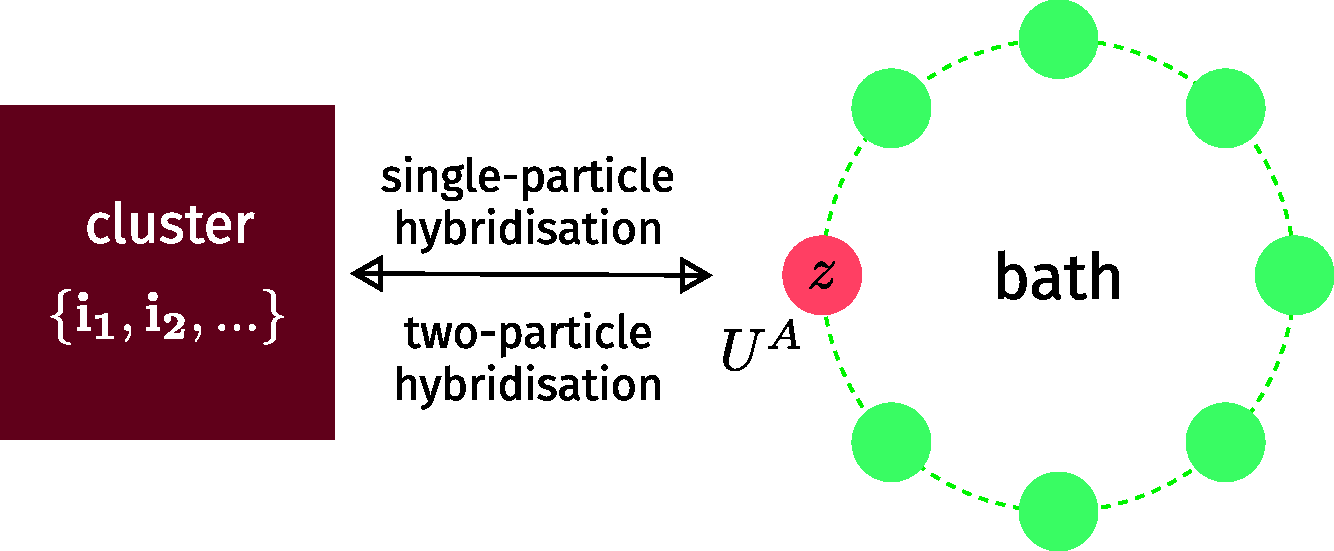
\includegraphics[width=0.95\textwidth]{figures/gen_siam.pdf}
\end{minipage}

\footcite{Schrieffer_Wolff,anderson_impurity_1961}

\end{frame}

\section{The Unitary Renormalization Group Method}
\label{method}
\begin{frame}[noframenumbering]{The Unitary Renormalization Group Method}
\footcite{anirbanurg1,anirbanurg2}

\only<1-3>{
\head{The General Idea}
\begin{minipage}{0.8\textwidth}
\begin{itemize}[<+->]
	\item Apply unitary many-body transformations to the Hamiltonian\\[10pt]
	\item Successively decouple high energy states\\[10pt]
	\item Obtain sequence of Hamiltonians and hence scaling equations
\end{itemize}
\end{minipage}
\begin{minipage}{0.15\textwidth}
\begin{figure}
	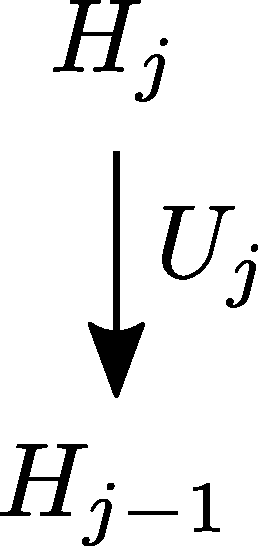
\includegraphics[width=0.7\textwidth]{figures/urg_schematic.pdf}
\end{figure}
\end{minipage}
}

\only<4>{
\head{Select a UV-IR Scheme}
\vspace*{\fill}

\begin{minipage}{0.5\textwidth}
\centering
\focus{UV shell}
\begin{gather*}
	\vec k_N ~~ \left(\text{zeroth RG step}\right)\\
\vdots\\ 
\vec k_j ~ ~ \left(j^\text{th} \text{ RG step}\right) \\
\vdots\\
\vec k_1 ~ ~ \left(\text{Fermi surface}\right)
\end{gather*}
\focus{IR shell}
\end{minipage}
\hspace*{\fill}
\begin{minipage}{0.4\textwidth}
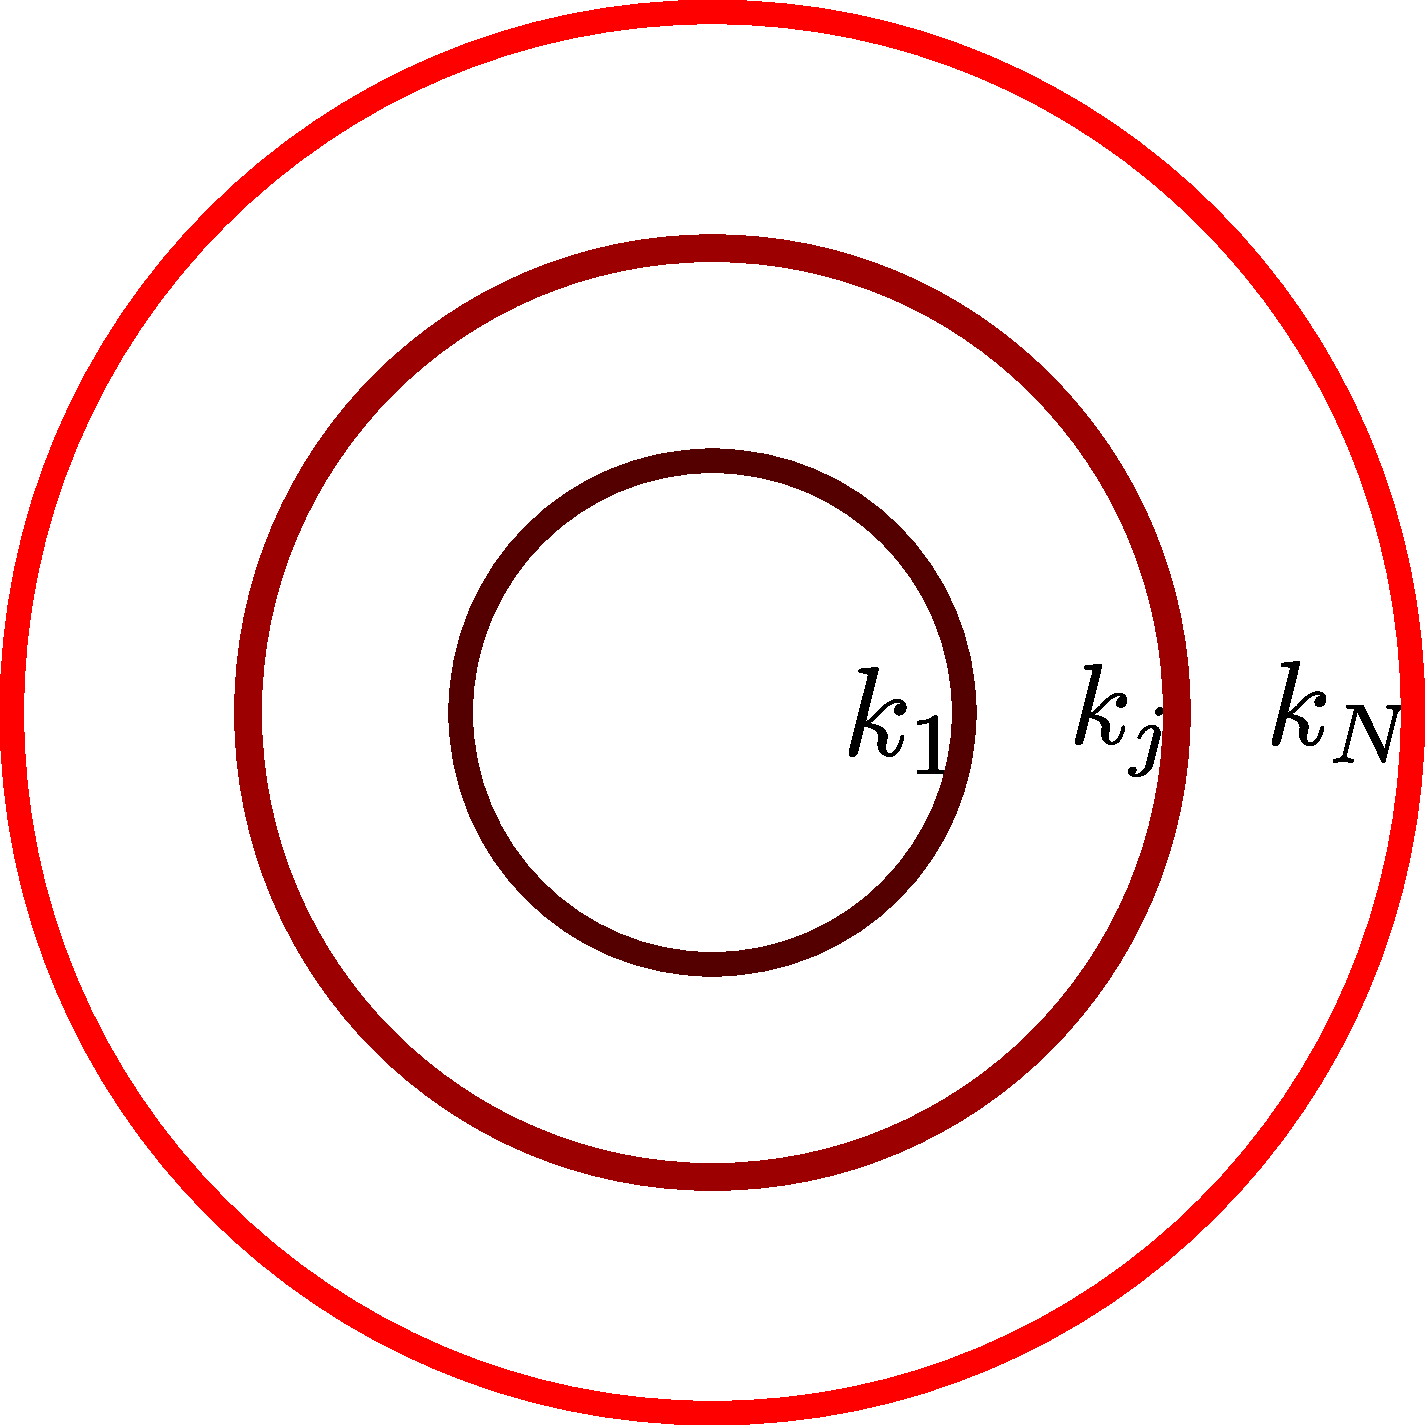
\includegraphics[width=0.9\textwidth]{figures/uv_ir_scheme.pdf}
\end{minipage}
\vspace*{\fill}
}

\only<5>{
\vspace*{-20pt}
\head{Write Hamiltonian in the basis of \(\vec k_j\)}
\vspace*{\fill}

\begin{minipage}{0.4\textwidth}
	\vspace*{-30pt}
	\[H_{(j)} = H_1 \hat n_j + H_0 \left(1 - \hat n_j\right) + c^\dagger_j T + T^\dagger c_j\]
\[
 {2^{j-1} \text{-dim.}} \longrightarrow \begin{cases}
	H_1, H_0 \longrightarrow \text{diagonal parts}\\
T \longrightarrow \text{off-diagonal part}
\end{cases}
\]
\[ (j) : j^\text{th} \text{ RG step}\]
\end{minipage}
\hspace*{\fill}
\begin{minipage}{0.5\textwidth}
\begin{figure}
	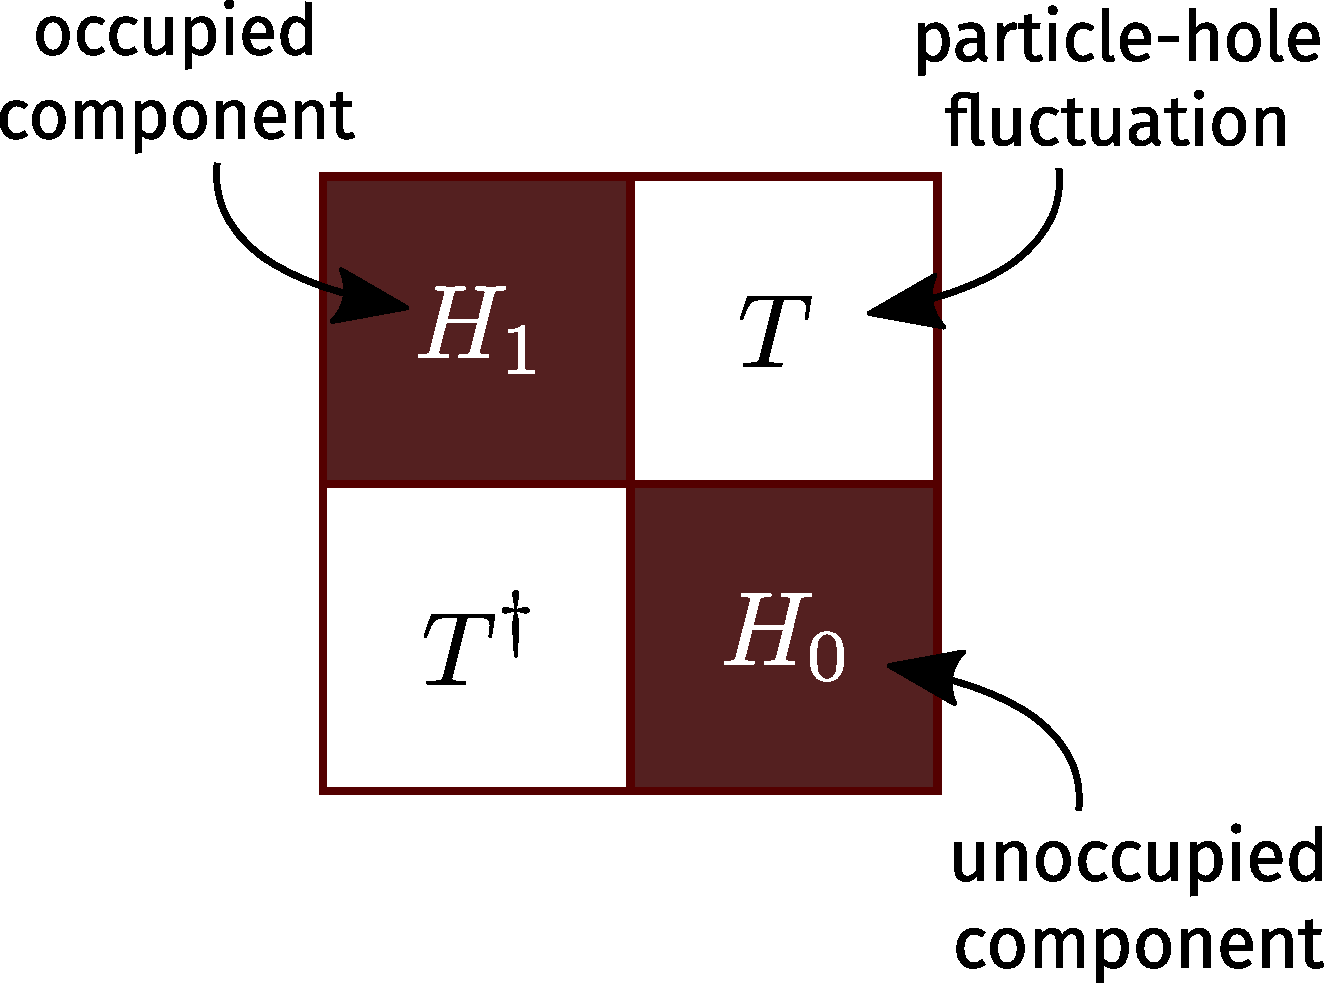
\includegraphics[width=0.9\textwidth]{figures/urg_ham.pdf}
\end{figure}
\end{minipage}
}
\only<6>{
\vspace*{-10pt}
\head{Rotate Hamiltonian and kill off-diagonal blocks}

\vspace*{\fill}

\begin{minipage}{0.45\textwidth}
\centering
\[H_{(j-1)} = U_{(j)} H_{(j)} U_{(j)}^\dagger\]
\[U_{(j)} = \frac{1}{\sqrt 2}\left(1 - \eta_{(j)} + \eta_{(j)}^\dagger\right), ~ ~ \left\{\eta_{(j)}, \eta^\dagger_{(j)}\right\} = 1 \]
\[ \eta^\dagger_{(j)} = \frac{1}{\hat \omega_{(j)} - H_D}c^\dagger_j T \Bigg \} \rightarrow {\text{many-particle}\atop{\text{rotation}}}\]
\[\hat \omega_{(j)} = \left(H_{1} + H_{0}\right)_{(j-1)} + \Delta T_{(j)}\]
\[\text{\focus{\Big(quantum fluctuation operator\Big)}}\]
\vspace*{\fill}
\end{minipage}
\hspace*{\fill}
\begin{minipage}{0.5\textwidth}
\begin{figure}
	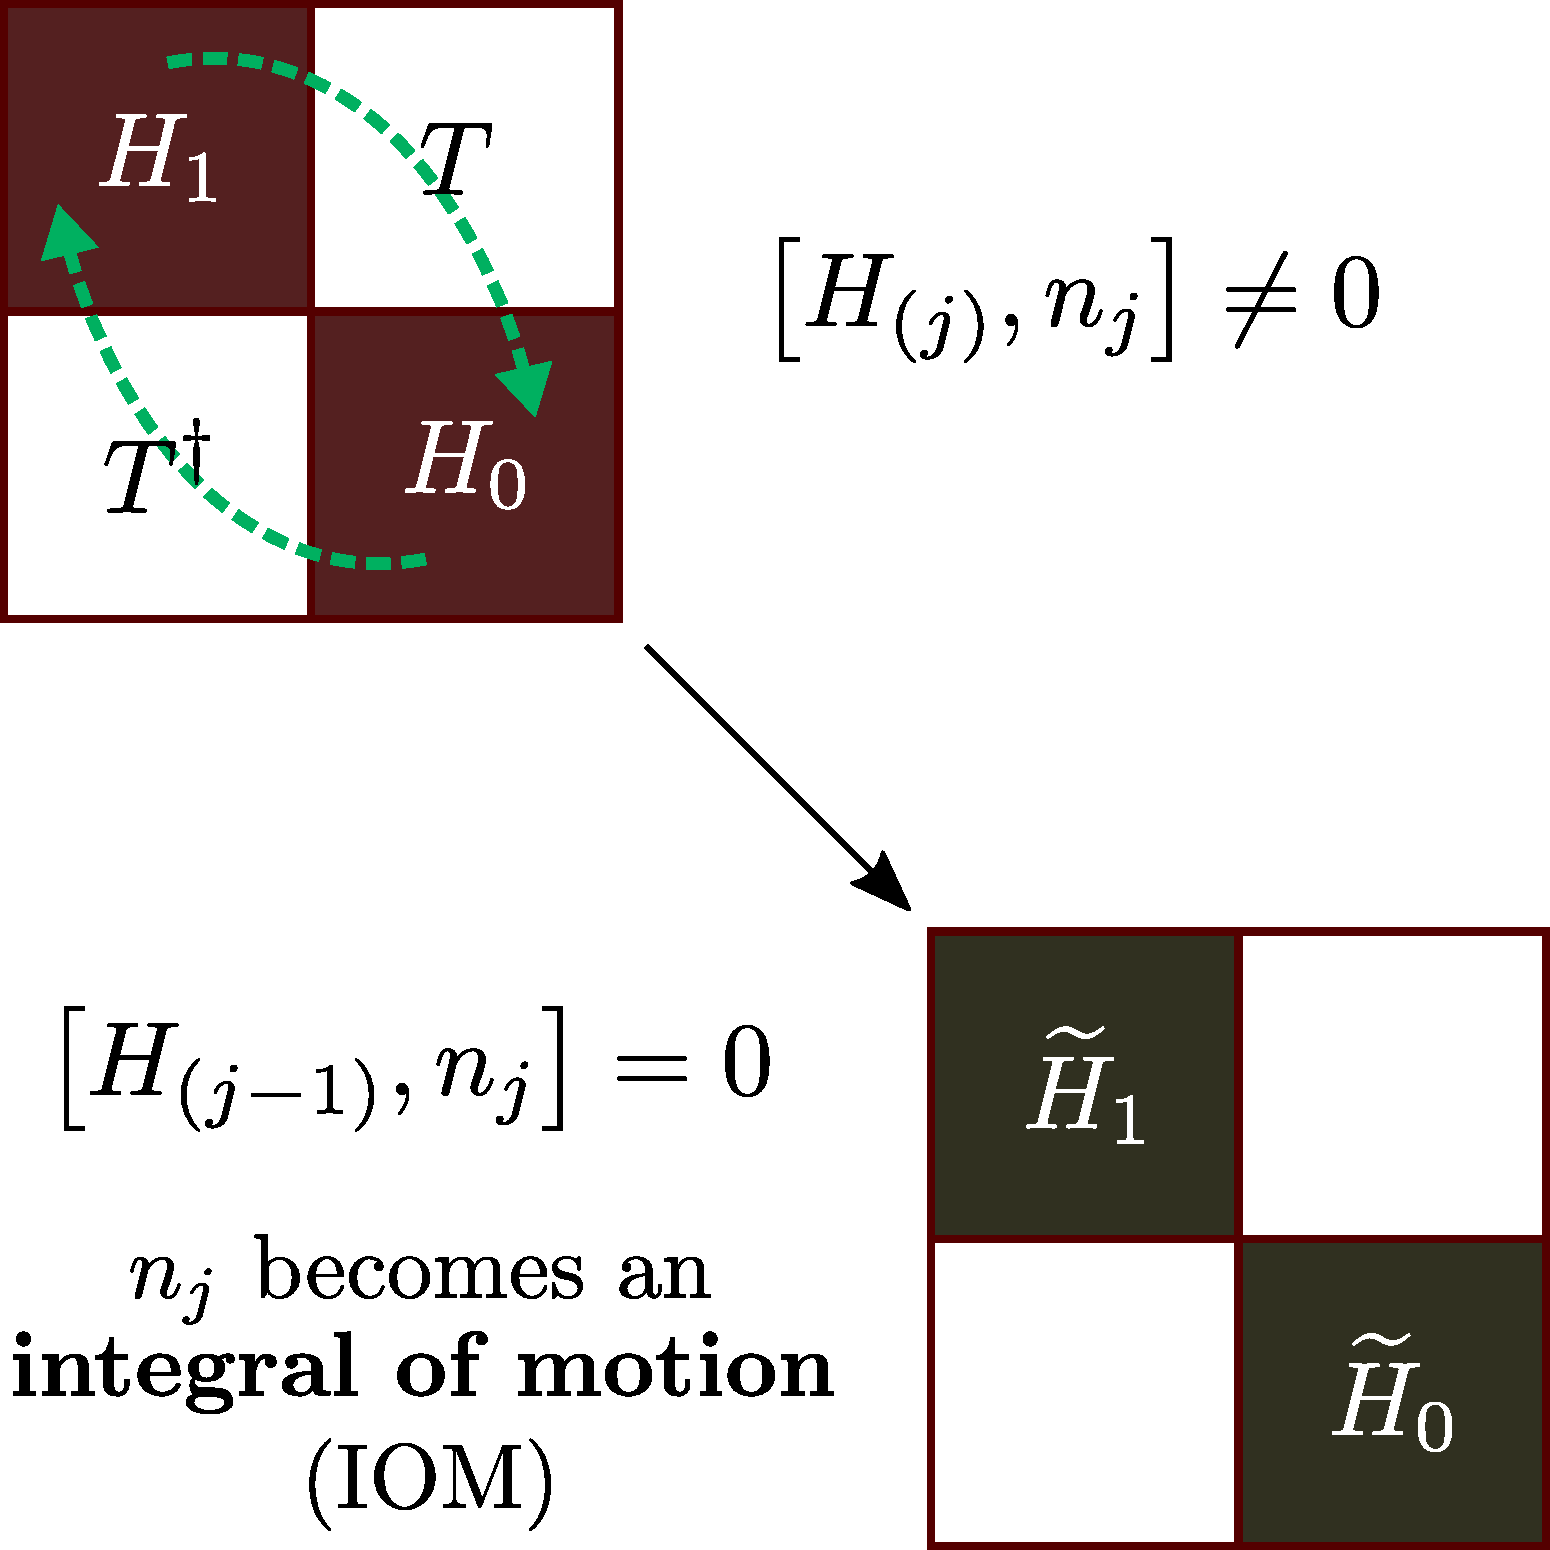
\includegraphics[width=0.8\textwidth]{figures/urg_rot.pdf}
\end{figure}
\end{minipage}
}

\only<7>{

\head{Repeat with renormalised Hamiltonian}

\begin{minipage}{0.53\textwidth}
	\[H_{(j-1)} = \widetilde H_1 \hat n_j + \widetilde H_0 \left(1 - \hat n_j\right)\]
	\[\widetilde H_1 = H_1 \hat n_{j-1} + H_0 \left(1 - \hat n_{j-1}\right) + c^\dagger_{j-1} T + T^\dagger c_{j-1}\]
\vspace*{\fill}
\end{minipage}
\hspace*{\fill}
\begin{minipage}{0.45\textwidth}
\begin{figure}
	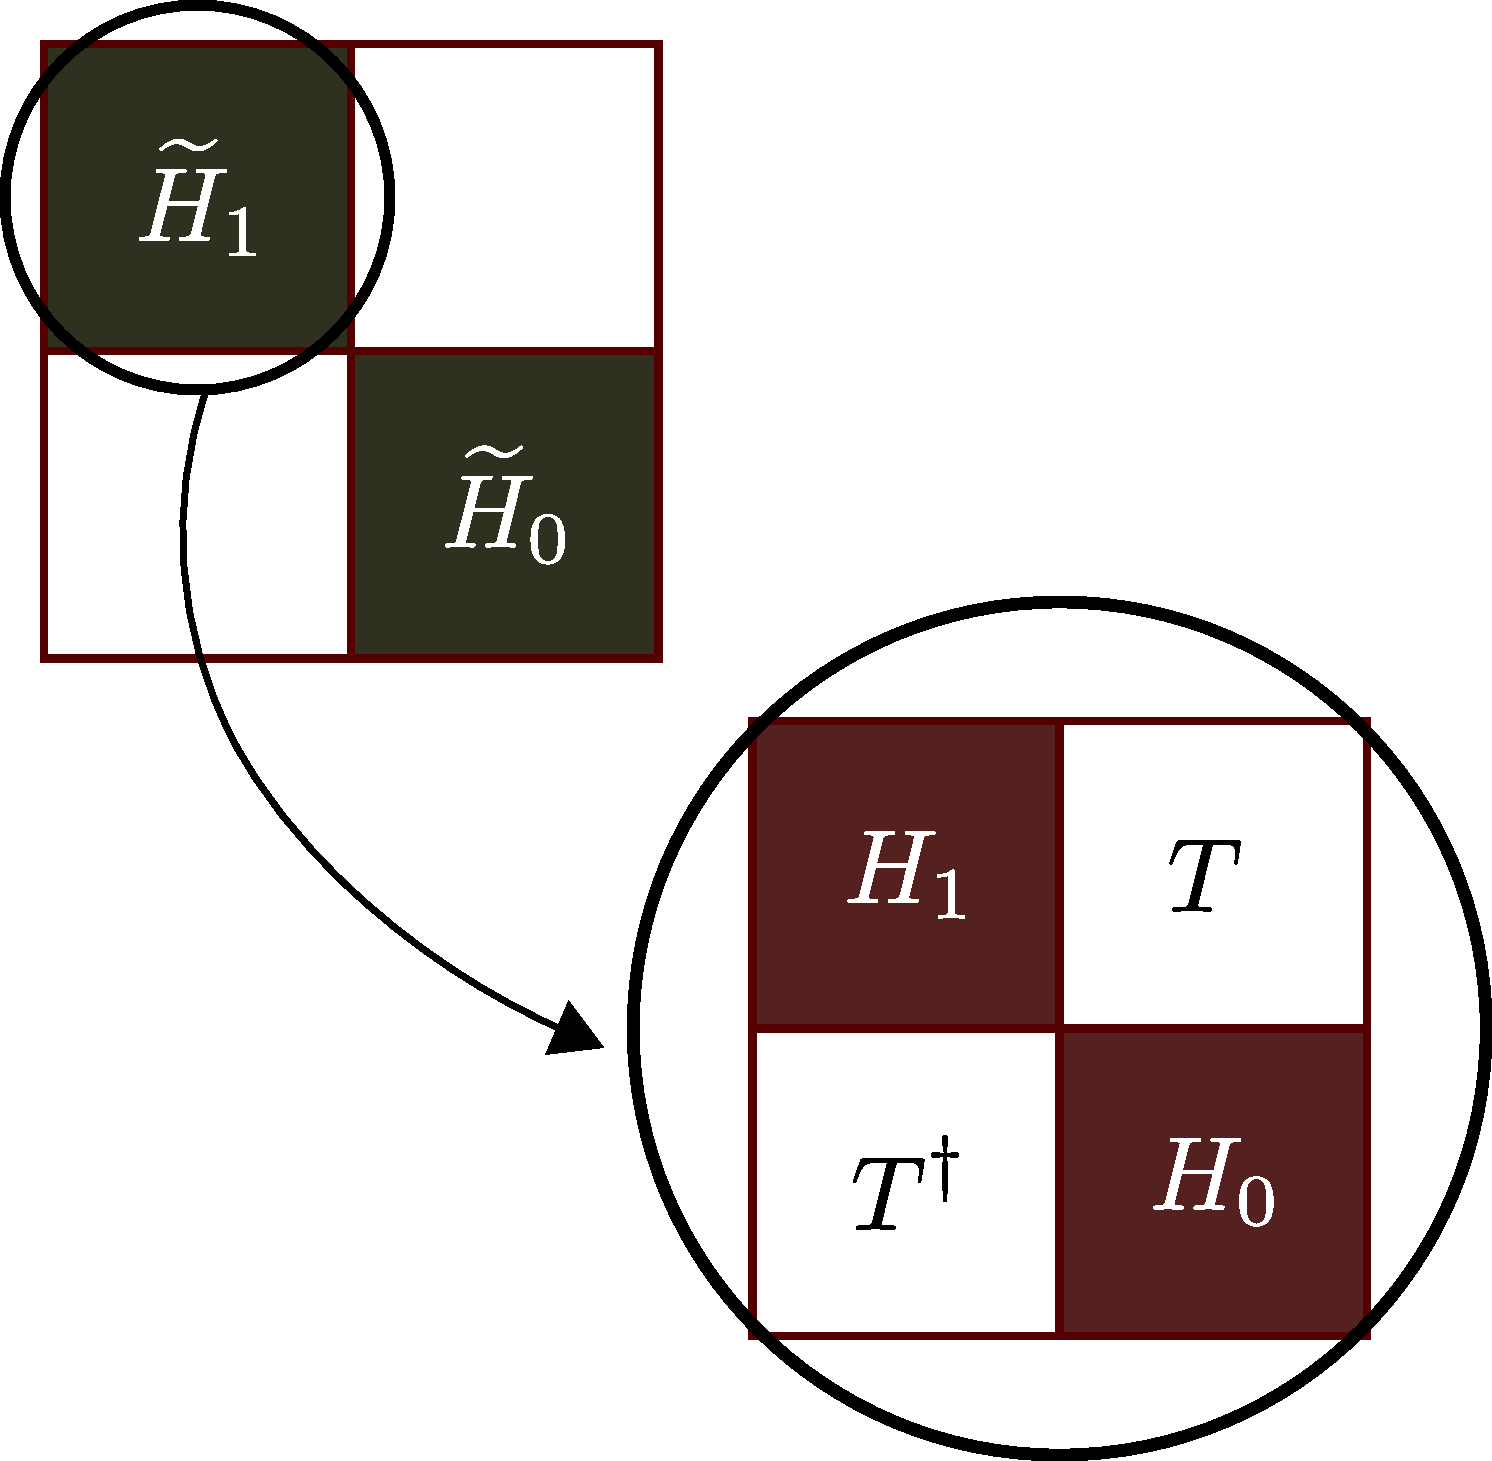
\includegraphics[width=\textwidth]{figures/urg_next.pdf}
\end{figure}
\end{minipage}
}

\only<8>{
\vspace*{-30pt}
\head{RG Equations and Denominator Fixed Point}

\vspace*{40pt}
\begin{minipage}{0.4\textwidth}
	\centering
\[ \Delta H_{(j)} = \left(\hat n_j - \frac{1}{2}\right) \left\{c^\dagger_j T, \eta_{(j)}\right\} \]
\[\eta^\dagger_{(j)} = \frac{1}{\hat \omega_{(j)} - H_D}c^\dagger_j T\] 
\[\text{{Fixed point:}}~ ~ ~\hat \omega_{(j^*)} - \left(H_D\right)^* = 0\]
\focus{eigenvalue of \(\hat \omega\) coincides with that of \(H\)}
\end{minipage}
\hspace*{\fill}
\begin{minipage}{0.58\textwidth}
	\centering
	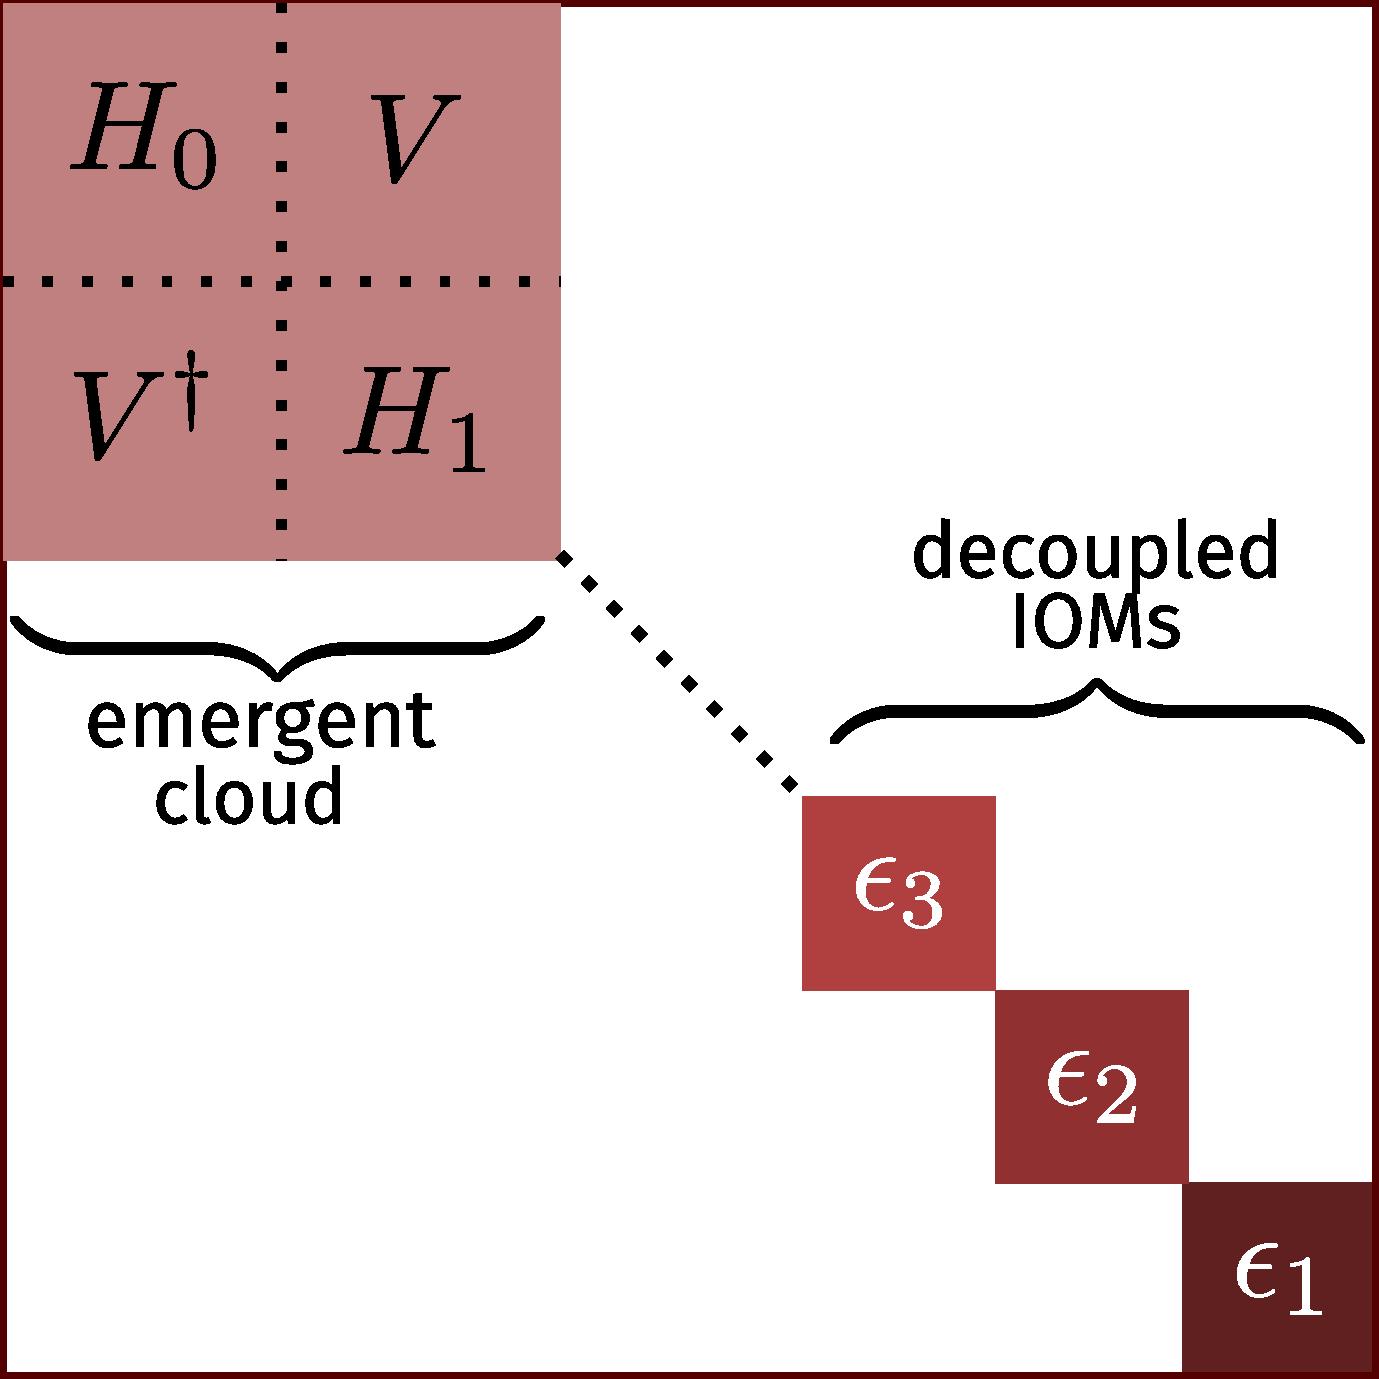
\includegraphics[width=0.65\textwidth]{figures/urg_ham_full.pdf}
\end{minipage}
\vspace*{\fill}
}
\end{frame}

\begin{frame}[noframenumbering]{The Unitary Renormalization Group Method}
\head{Novel Features of the Method}
% \hspace*{-20pt}
\begin{minipage}{0.65\textwidth}
\begin{itemize}[<+->]
	\item \focus{Quantum fluctuation scale} \(\hat \omega\)	that tracks all orders of renormalisation\\[10pt]
	\item Finite-valued fixed points for finite systems - leads to \focus{emergent degrees of freedom}\\[10pt]
	\item \focus{Spectrum-preserving} unitary transformations - partition function does not change\\[10pt]
	\item Tractable low-energy effective Hamiltonians - allows \focus{renormalised perturbation theory} around them 
\end{itemize}
\end{minipage}
\hspace*{\fill}
\begin{minipage}{0.3\textwidth}
\begin{flushleft}
	\(H_{(j-1)} = U_{(j)} H_{(j)} U_{(j)}^\dagger\)\\[15pt]
	\(U_{(j)} = \frac{1}{\sqrt 2}\left(1 - \eta_{(j)} + \eta_{(j)}^\dagger\right) \)\\[15pt]
	\( \eta^\dagger_{(j)} = \frac{1}{\hat \omega_{(j)} - H_D}c^\dagger_j T\)\\[15pt]
	\( \Delta H_{(j)} = \left(\hat n_j - \frac{1}{2}\right) \left\{c^\dagger_j T, \eta_{(j)}\right\} \)
\end{flushleft}
\end{minipage}
\end{frame}
\section{URG Analysis: \(U_b=0\)}
\label{urg-1}
\begin{frame}[noframenumbering]{\(U_b = 0:\) Flow towards strong-coupling}
\centering
% \vspace*{-10pt}
{\(\mathbf{U > 0, J > 0}\)}

\vspace*{10pt}

\only<+>{
\centering

{\large \(\Delta V = \frac{3n_j VJ}{8}\left(\frac{1}{|d_2|} + \frac{1}{|d_1|}\right) > 0\), ~ ~ \(\Delta J = \frac{n_j J^2}{|d_2|} > 0\)}

{\large \(d_0 = \omega - \frac{D}{2} - \frac{U}{2} + \frac{K}{4}, \quad d_1 = \omega - \frac{D}{2} + \frac{U}{2} + \frac{J}{4}\), ~ ~
\(d_2 = \omega - \frac{D}{2} + \frac{J}{4}\)}

\hspace*{-50pt}
\vspace*{-20pt}

	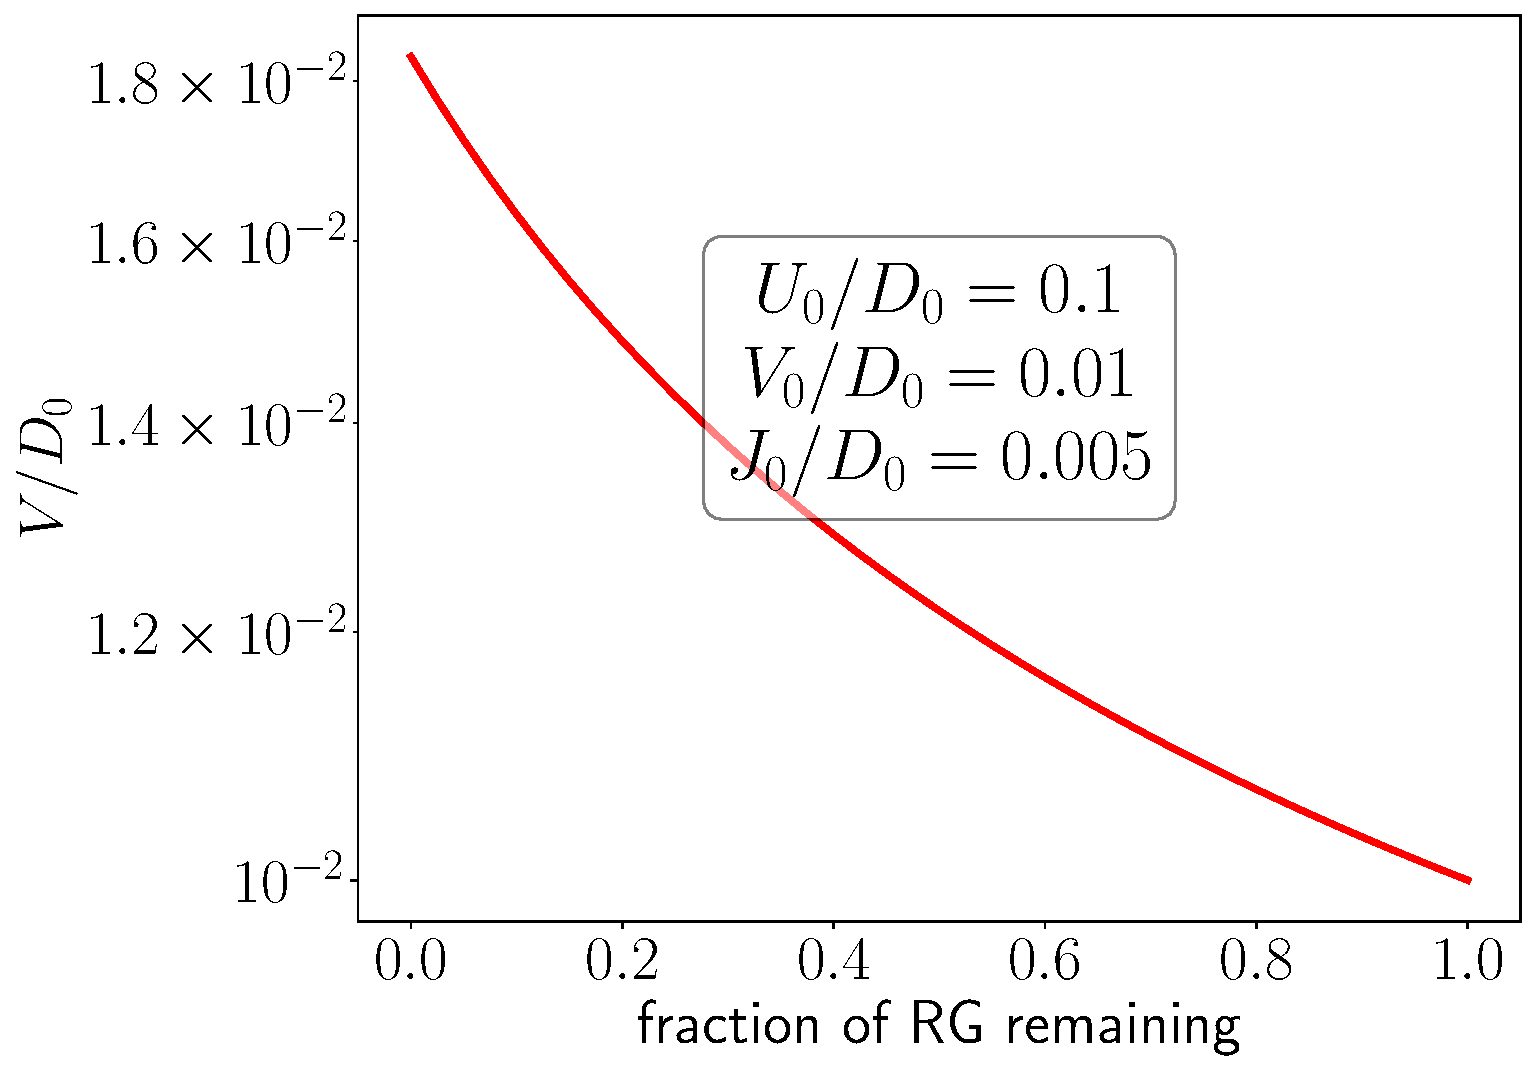
\includegraphics[width=0.49\textwidth]{figures/U_irr,U>0,V.pdf}
	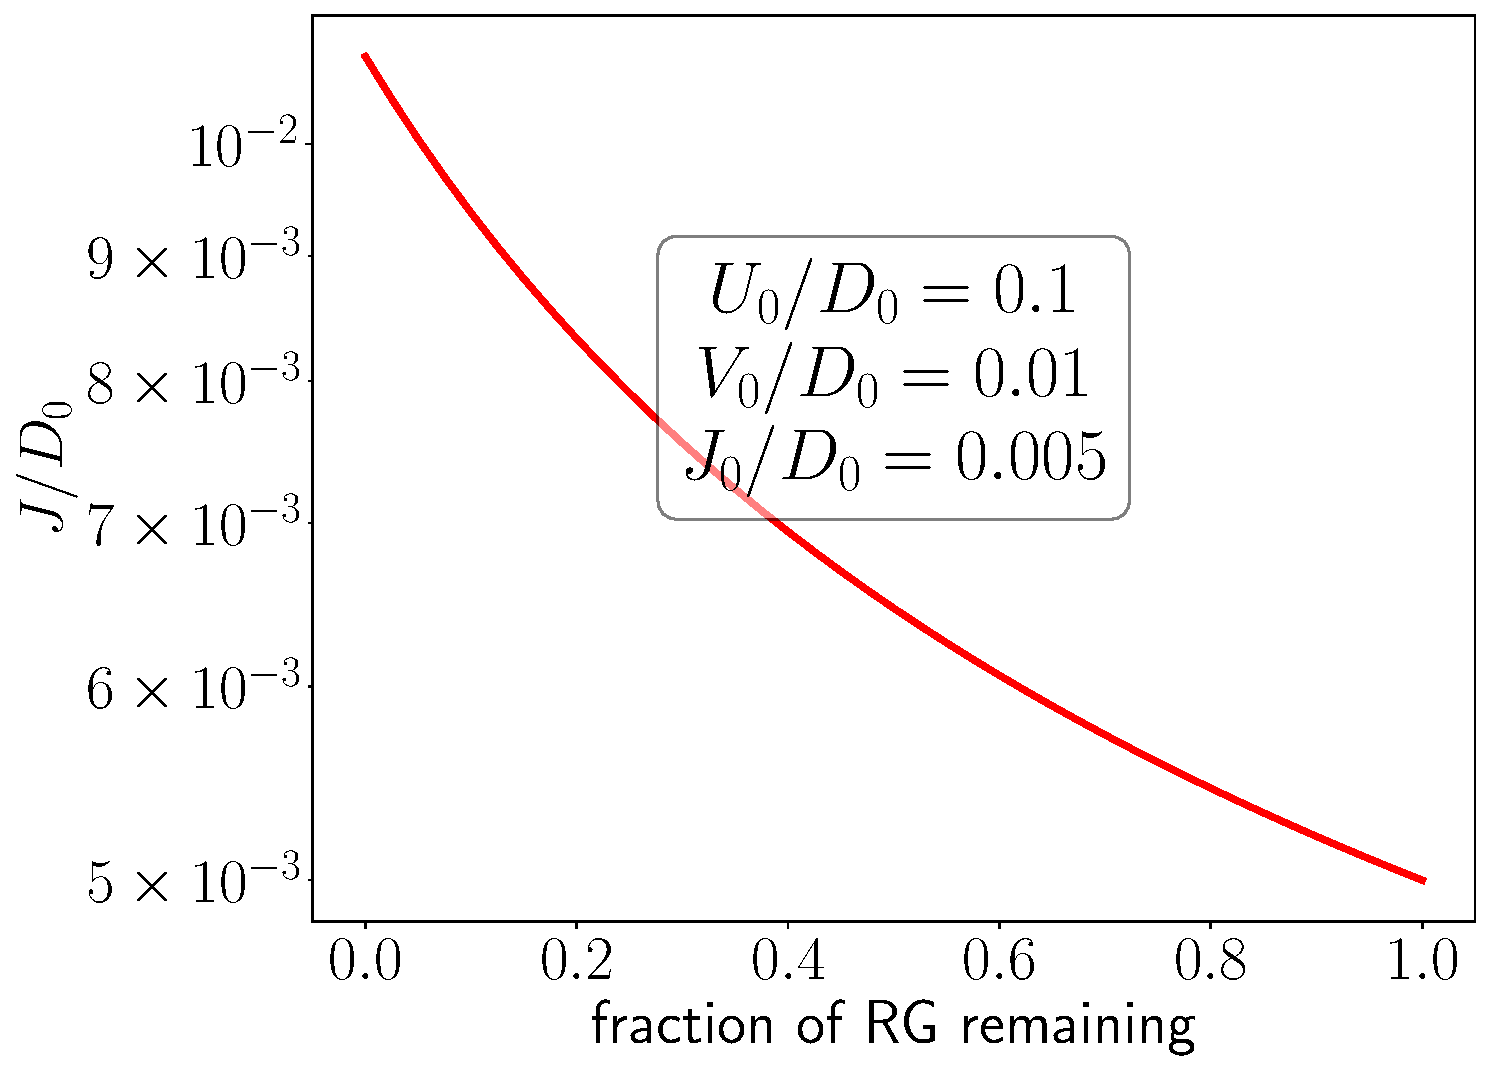
\includegraphics[width=0.49\textwidth]{figures/U_irr,U>0,J.pdf}
}
\only<+>{
{\large \(\Delta U = 4V^2 n_j\left(\frac{1}{d_1} - \frac{1}{d_0}\right) - n_j\frac{J^2}{d_2}\)}

% \vspace*{-10pt}

\begin{minipage}{0.49\textwidth}
\centering
{\large\( V > J\)}

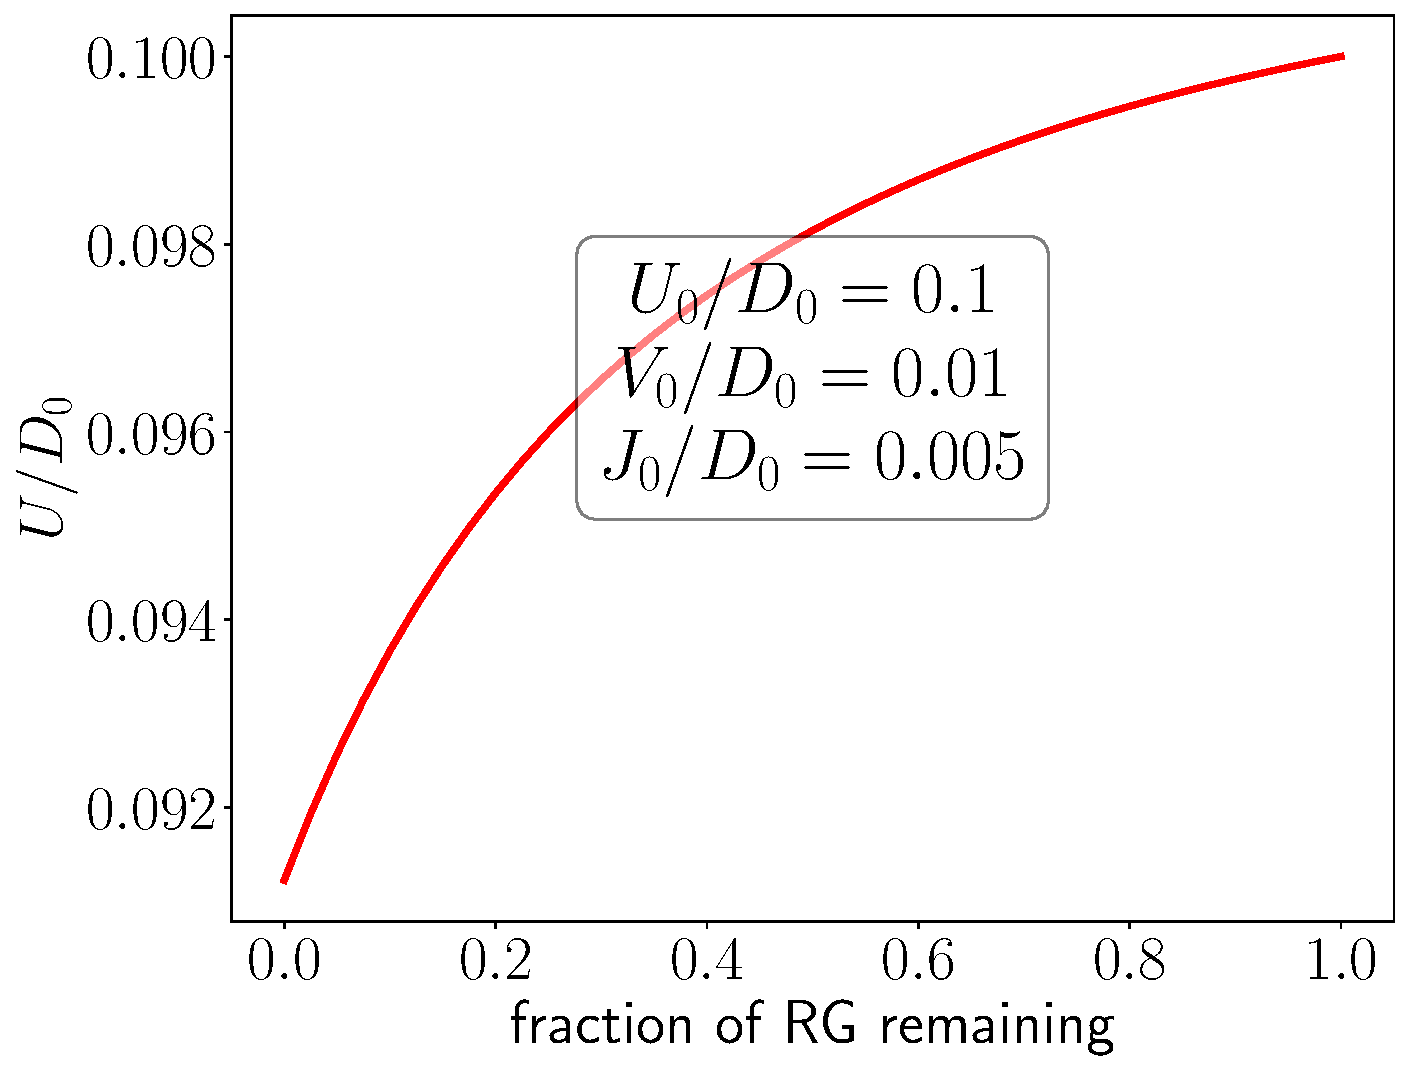
\includegraphics[width=\textwidth]{figures/U_irr,U>0,U.pdf}
\end{minipage}
\begin{minipage}{0.49\textwidth}
\centering
{\large\( V < J\)}

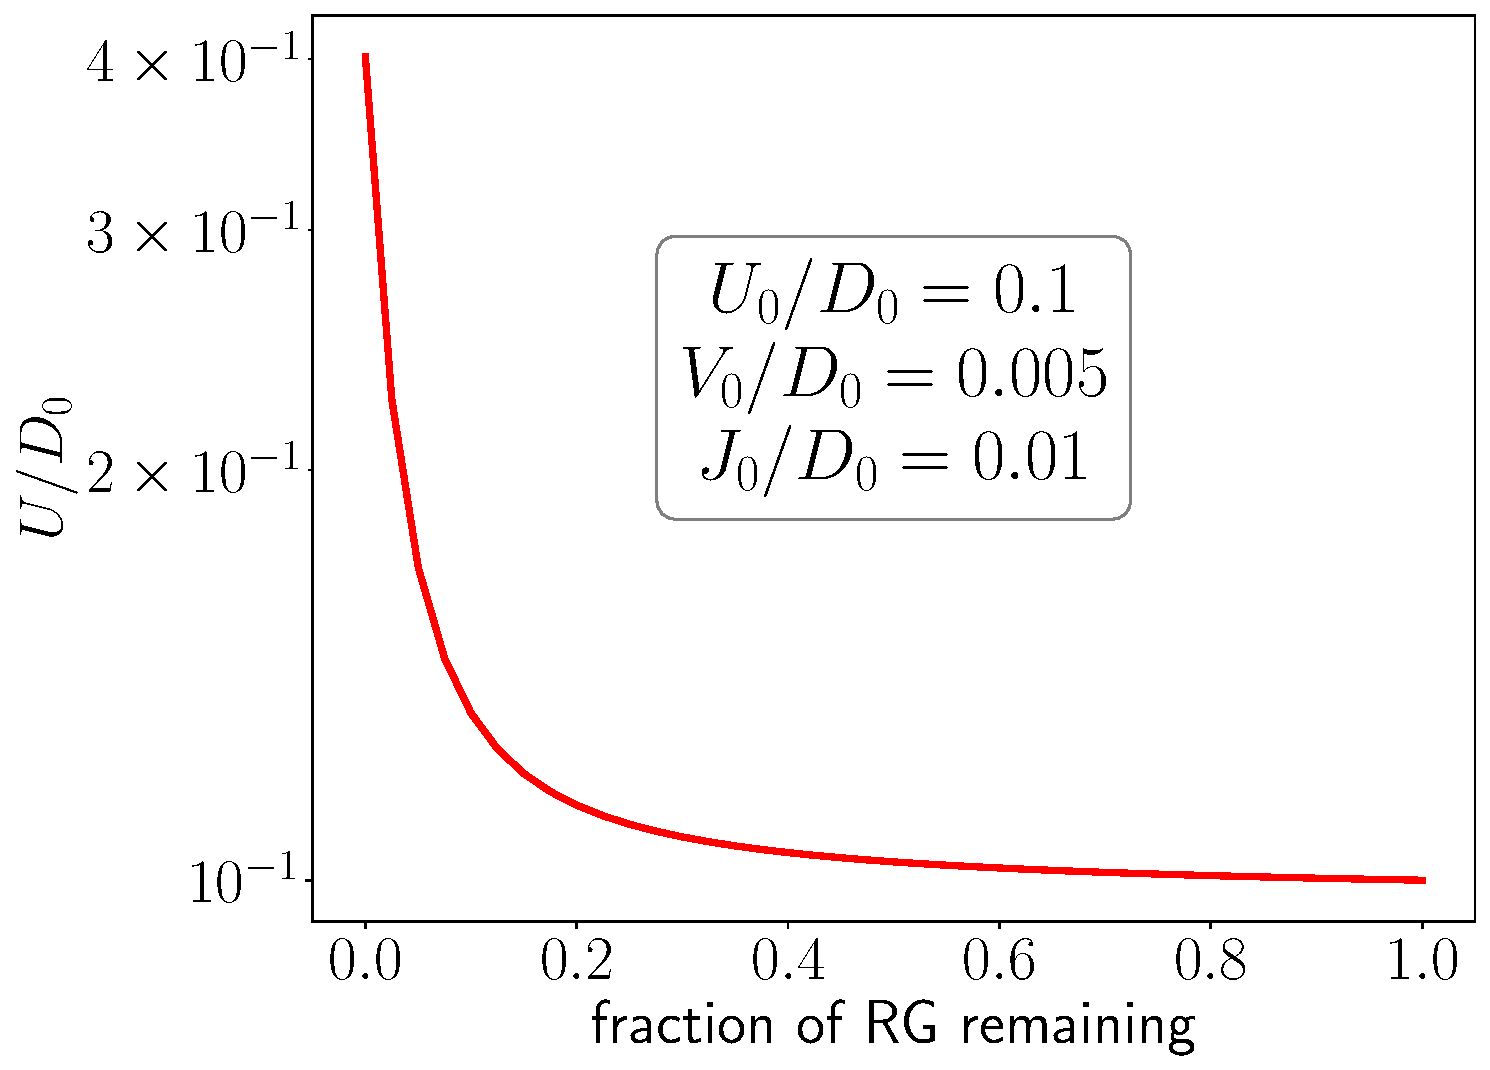
\includegraphics[width=\textwidth]{figures/U_rel,U>0,U.pdf}
\end{minipage}
}

\end{frame}

\begin{frame}[noframenumbering]{\(U > 0\) Fixed point Hamiltonian}
\begin{minipage}{0.48\textwidth}
	\[H^* = \sum_{k < k^*,\sigma}\epsilon_{k}\hat{n}_{k\sigma} ~ + \frac{U^*}{2}\left(\hat n_{d \uparrow} - \hat n_{d \downarrow}\right)^2 ~ + J^* \vec{S}_d\cdot \vec{s}_<\]
	\[+ ~ V^* \sum_{k < k^*,\sigma}\left(c^\dagger_{d\sigma}c_{k\sigma} + \text{h.c.}\right)\]

	\vspace*{20pt}
	\[\vec{s}_< = \frac{1}{2}\sum_{k,k^\prime < k^*}c^{\dagger}_{k\alpha}\vec{\sigma}_{\alpha\beta}c_{k^\prime,\beta}\]
\end{minipage}
\begin{minipage}{0.5\textwidth}
	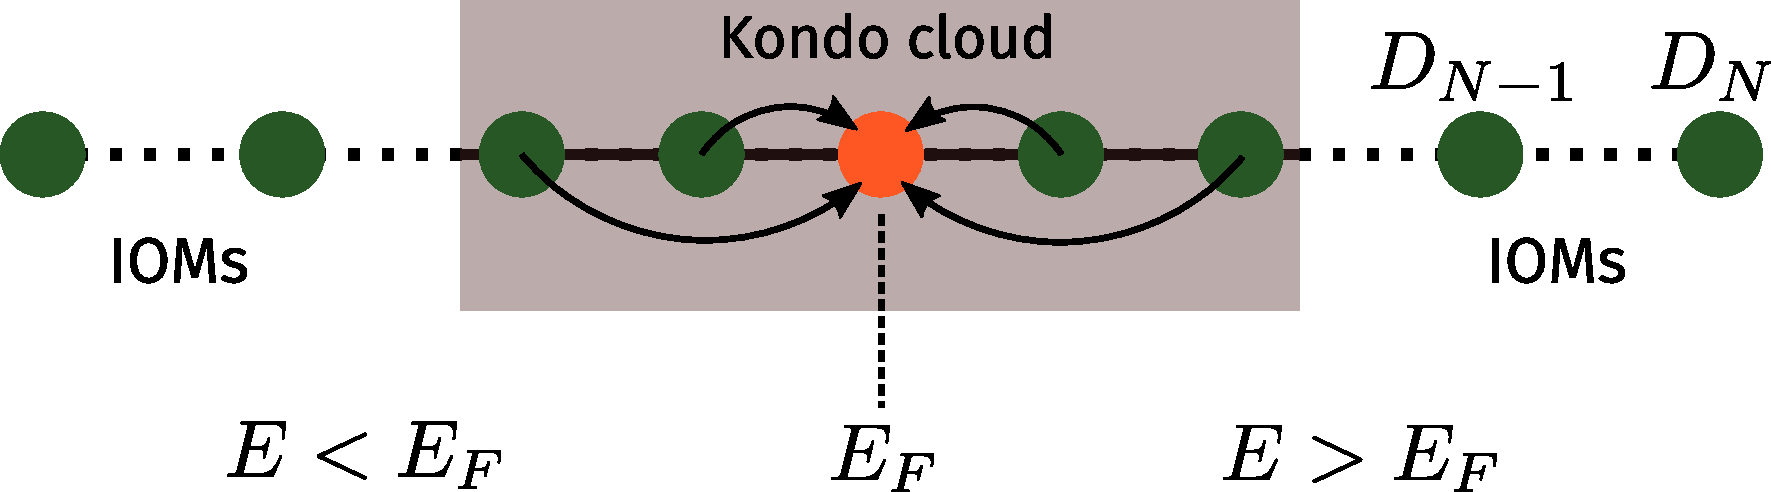
\includegraphics[width=\textwidth]{figures/kondo_fp_1D.pdf}
\end{minipage}
\end{frame}

\begin{frame}[noframenumbering]{Impurity Spectral Function}
\centering

\focus{no gap} at arbitrarily large $U$

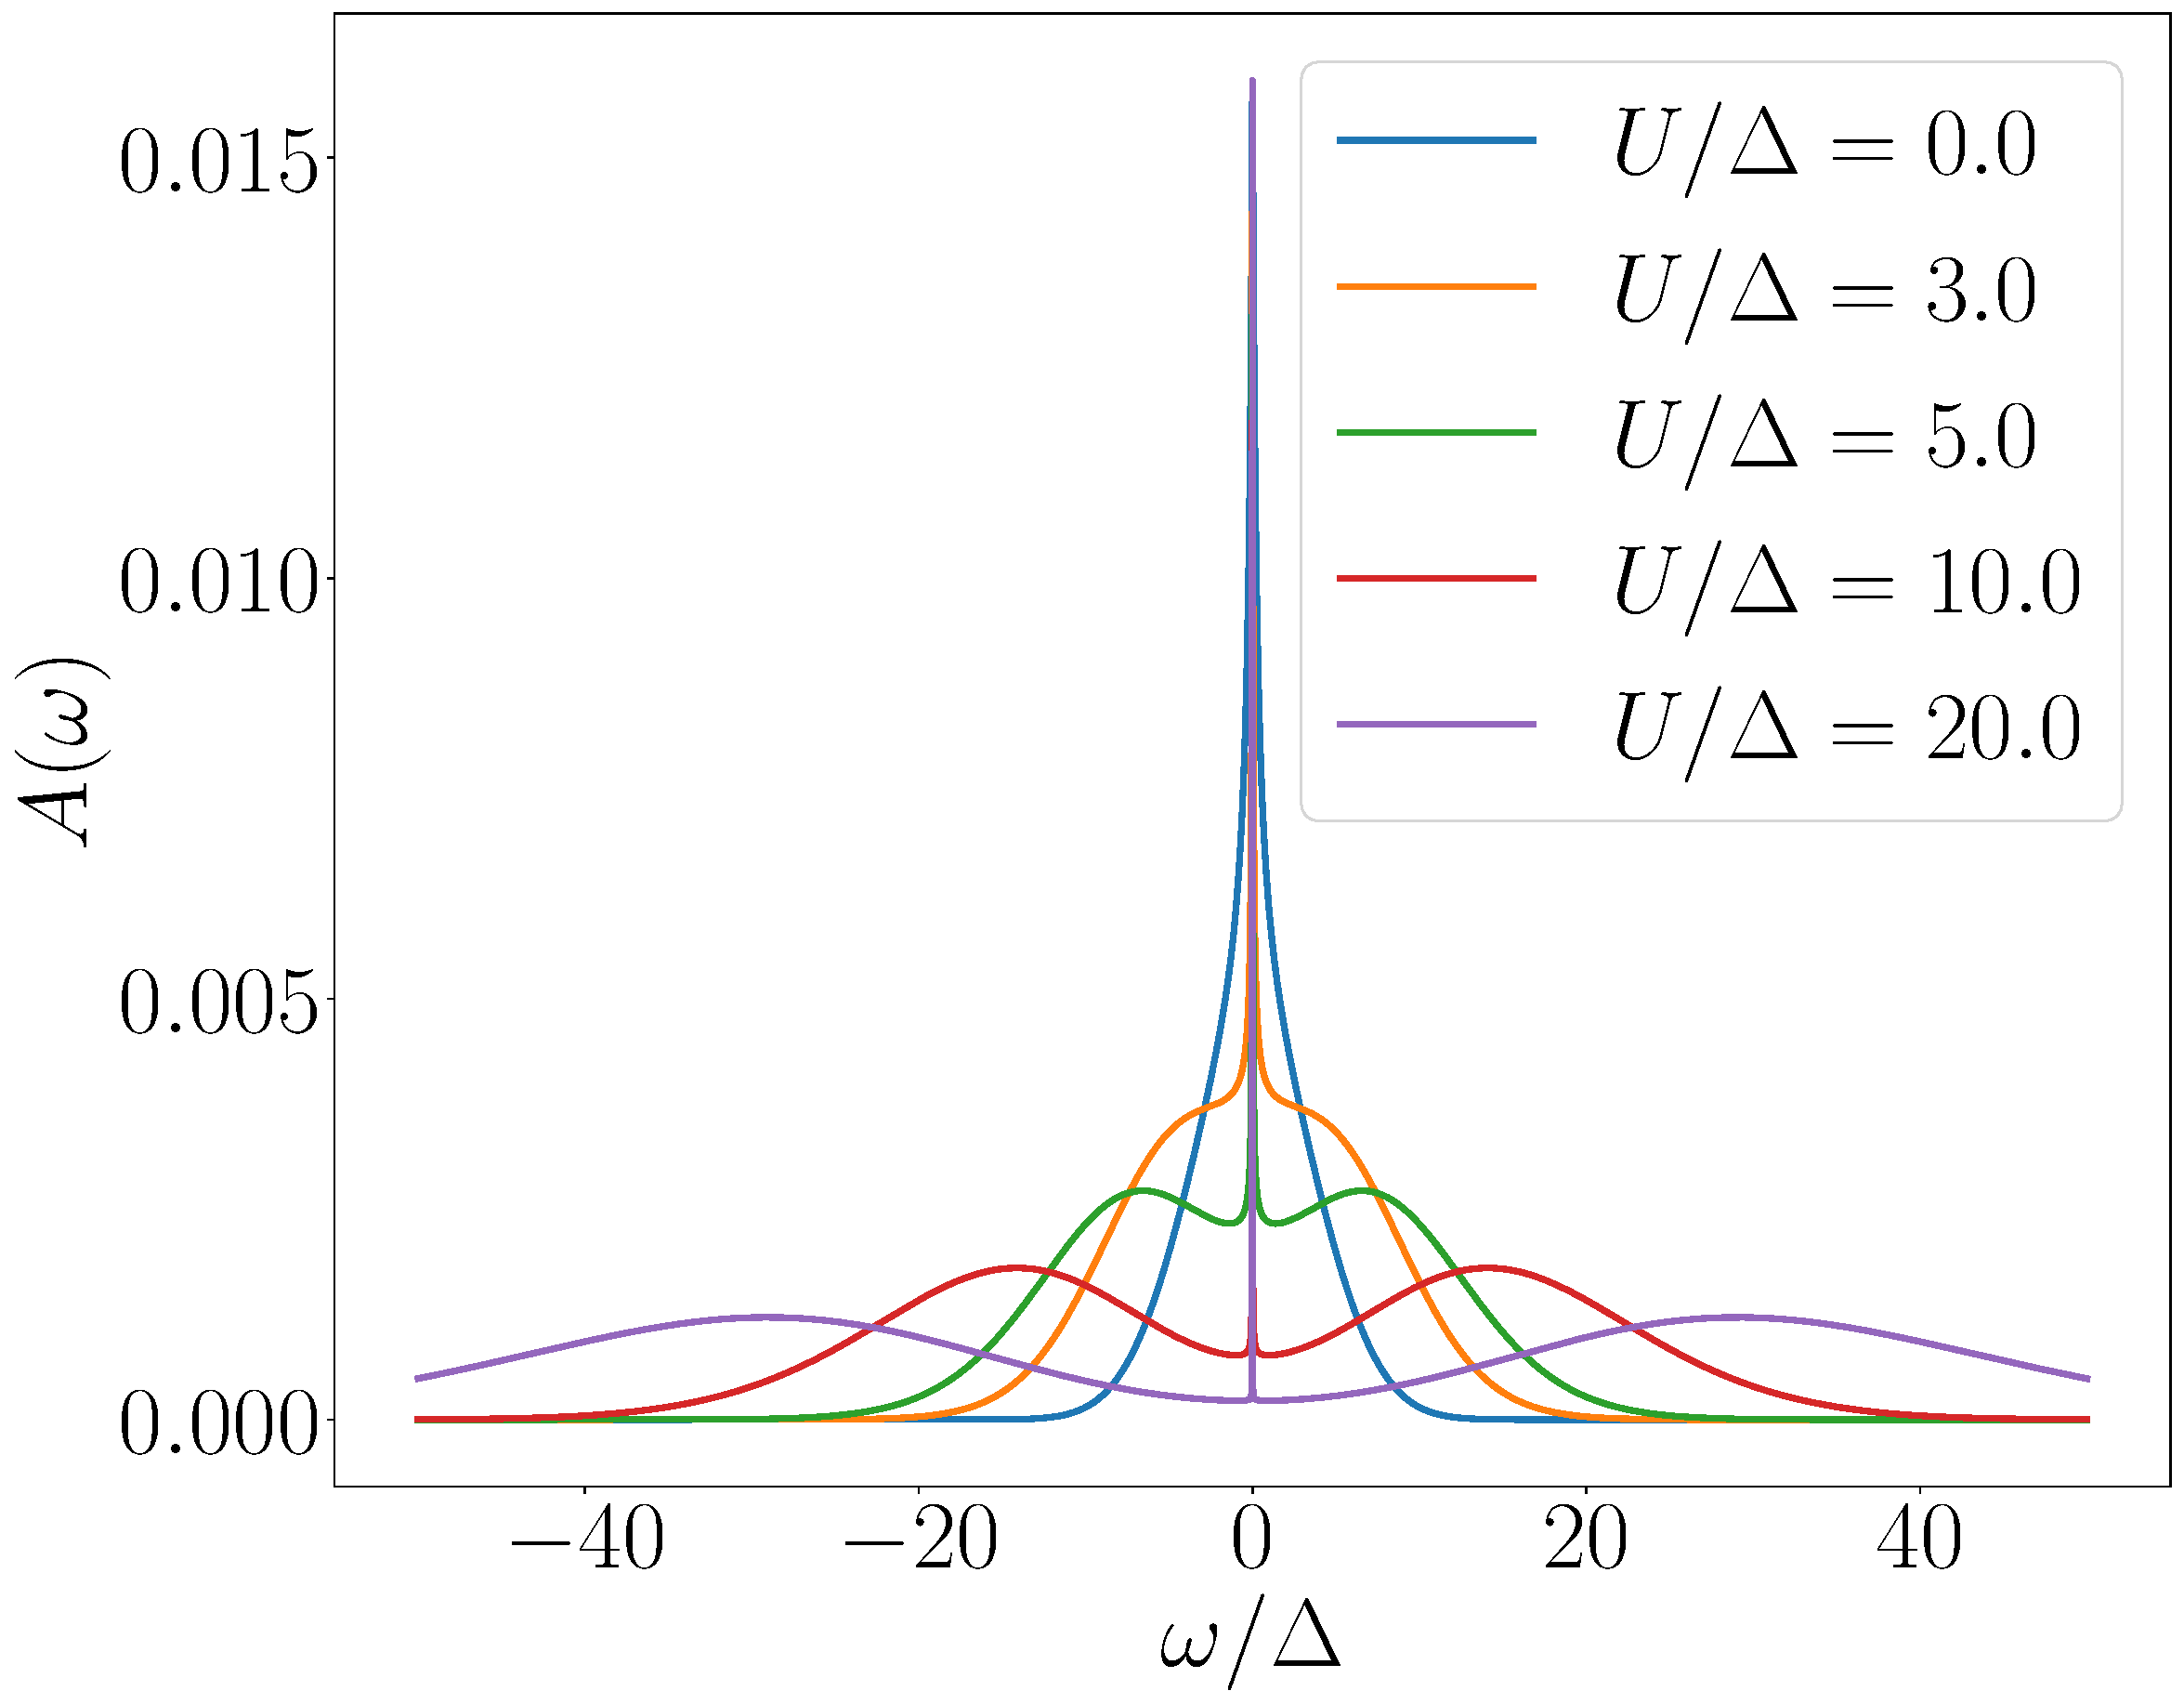
\includegraphics[width=0.6\textwidth]{./figures/gen_siam_spec_func.pdf}

\end{frame}

\section{URG Analysis: \(U_b \neq 0\)}
\label{urg-2}

\begin{frame}[noframenumbering]{\(U > 0\) RG Equations}

\begin{itemize}[<+->]
	\item \(U_b\) is \focus{marginal}: ~ ~ ~\(\Delta U_b = 0\)
	\item Spin-exchange couling \(J\) can now be \focus{driven irrelevant} by \(U_b\): 
	\begin{equation*}
	\Delta J = -\frac{n_j J\left(J + 4U_b\right)}{d_2} \longrightarrow \begin{cases}
	\text{\textcolor{blue}{relevant} when }J+4U_b > 0\\
	\text{\textcolor{red}{irrelevant} when }J+4U_b < 0\\
	\end{cases}
	\end{equation*}
	\item Same can be said for the hybridisation \(V\):
	\begin{equation*}
	\Delta V = -\frac{3n_j V}{8}\left[\left(J + \frac{4U_b}{3}\right) \left(\frac{1}{d_2} + \frac{1}{d_1}\right) + \frac{4U_b}{3}\left(\frac{1}{d_3} + \frac{1}{d_0}\right)\right] \longrightarrow \begin{cases}
	\text{\textcolor{blue}{rel.},}J+4U_b > 0\\
	\text{\textcolor{red}{irrel.},}J+4U_b < 0\\
	\end{cases}
	\end{equation*}
	\item \focus{\(U\) can be relevant if \(J\) decays slower than \(V\)}; needs to be checked numerically
\end{itemize}
\end{frame}

\begin{frame}[noframenumbering]{\(U > 0\) Phase Diagram}
\hspace*{-15pt}
\begin{minipage}{0.5\textwidth}
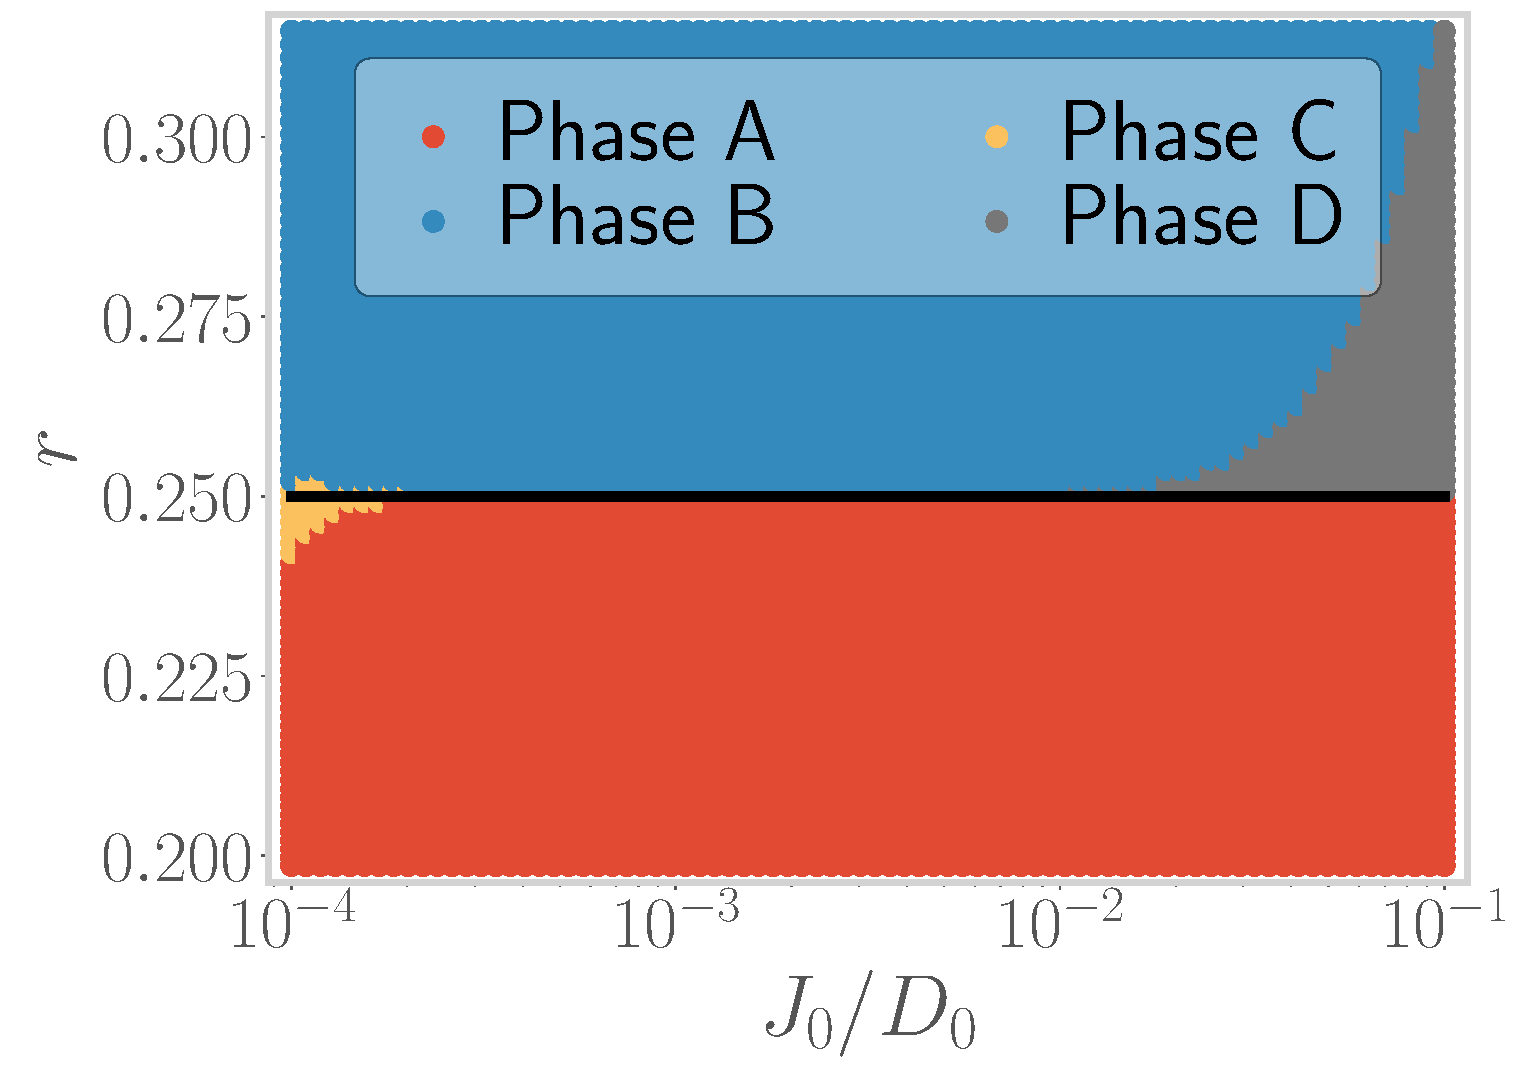
\includegraphics[width=\textwidth]{./figures/phase-map-MIT.pdf}
\end{minipage}
\begin{minipage}{0.52\textwidth}
	\begin{itemize}[<+->]
		\item black line: \focus{critical points} at \(U_b^* = -J^*/4\)\\[10pt]
		\item blue: \focus{screened} impurity (strong-coup.)\\[10pt]
		\item red: \focus{unscreened} local mom. (\(J=V=0\))\\[10pt]
	\item gray: imp. level absent (\(U=J=V=0\))\\[10pt]
	\item green: \(J\) vanishes (\(J < U\))
	\end{itemize}
\end{minipage}

\vspace*{-10pt}
\hspace*{\fill}
\begin{minipage}{0.3\textwidth}
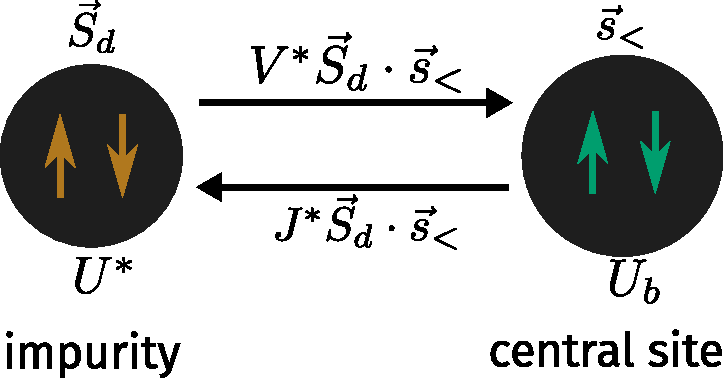
\includegraphics[width=\textwidth]{./figures/zeromode.pdf}
\end{minipage}
\hspace*{\fill}
\begin{minipage}{0.55\textwidth}
\only<2>{
\[\Delta J>0,\Delta V>0,\Delta U <0, ~ ~ ~ J^* \gg V^* \gg U^*\]
\[\frac{1}{\sqrt 2}\left(\ket{\uparrow,\downarrow} - \ket{\downarrow,\uparrow}\right) \]
}
\only<3>{
\[\Delta J<0,\Delta V<0,\Delta U >0, ~ ~ ~ J^* = V^* = 0, U^* \geq 0\]
\[\left\{\ket{\uparrow}, \ket{\downarrow}\right\} \otimes \left\{\ket{0}, \ket{2}\right\} \]
}
\only<4>{
\[\Delta J<0,\Delta V<0,\Delta U < 0, ~ ~ ~ J^* = V^* = U^* = 0\]
\[\left\{\ket{\uparrow}, \ket{\downarrow}, \ket{0}, \ket{2} \right\} \otimes \left\{\ket{0}, \ket{2}\right\} \]
}
\only<5>{
\[J^* < U^* < V^*\]
\[\frac{c}{\sqrt 2}\left(\ket{\uparrow,\downarrow} - \ket{\downarrow,\uparrow}\right) + \frac{\sqrt{1 - c^2}}{\sqrt 2}\left(\ket{2,0} + \ket{0,2}\right)\]
}
\end{minipage}
\end{frame}

\section{Evolution of two-site ground state and correlations across the transition}
\label{transition}

\begin{frame}[noframenumbering]{Overlap of ground state against spin singlet and charge triplet zero states}
	\centering
\only<1>{\(J_0/D_0 = 10^{-4}\)

\vspace*{-20pt}
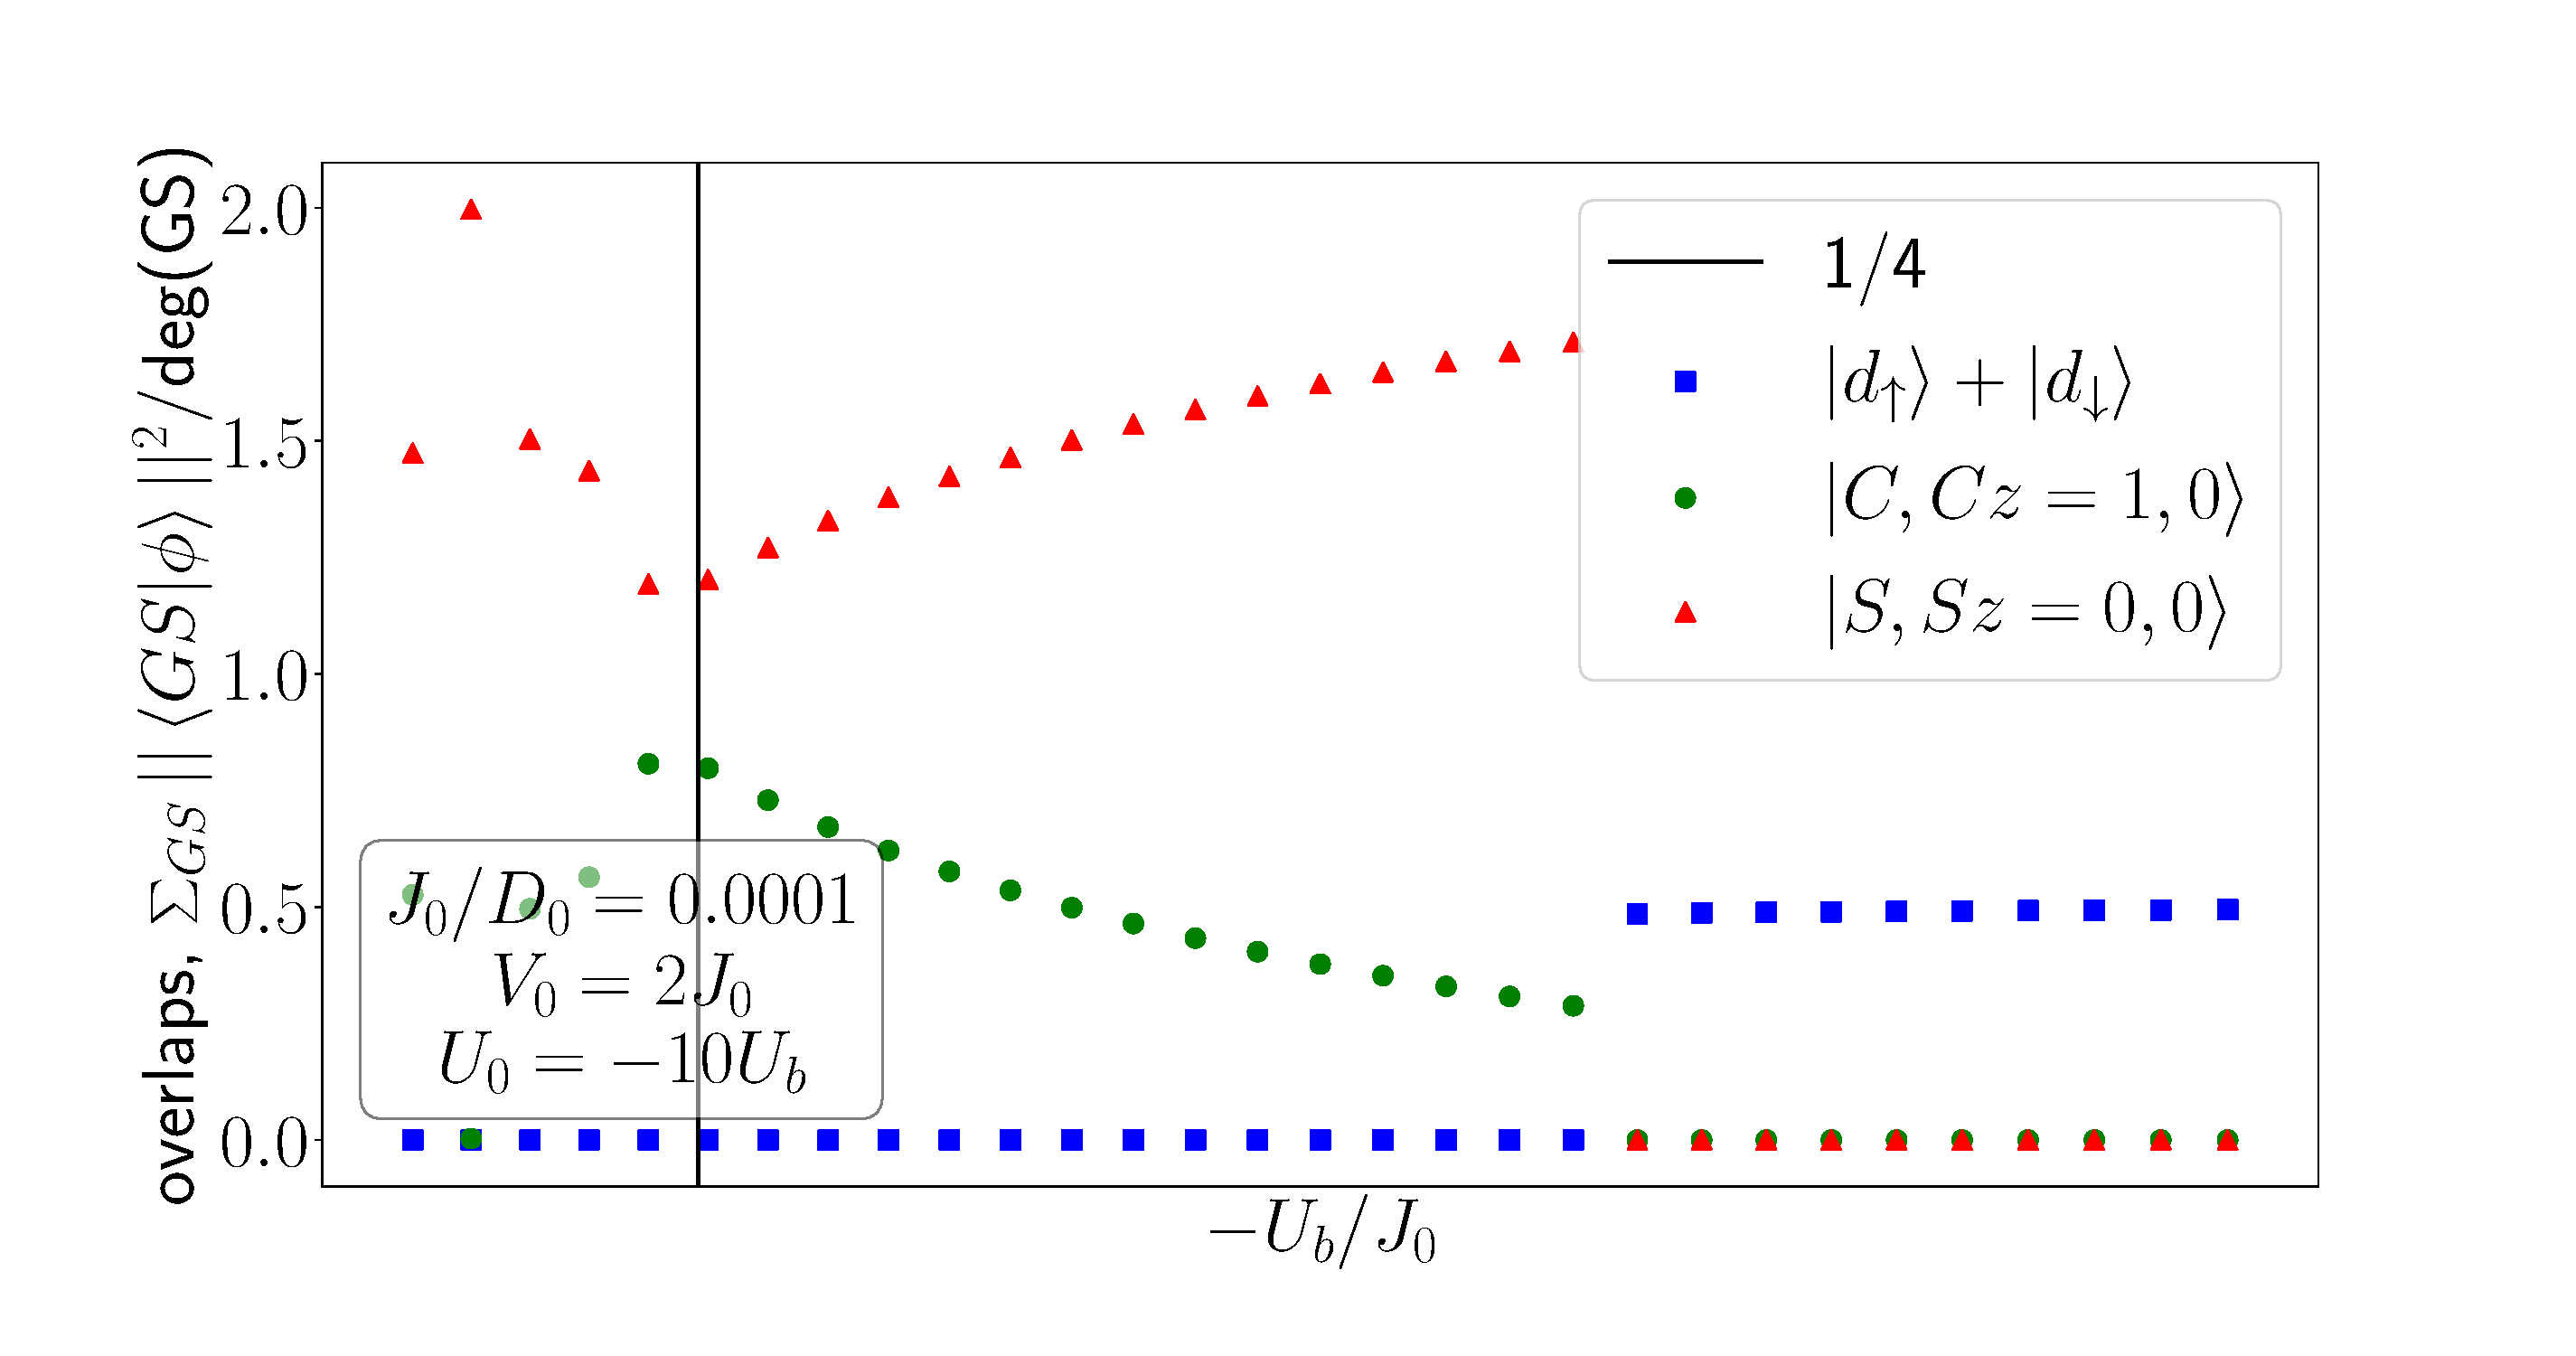
\includegraphics[width=\textwidth]{./figures/overlaps_gs-J=0.100.pdf}
}

\only<2>{\(J_0/D_0 = 10^{-2}\)

\vspace*{-20pt}
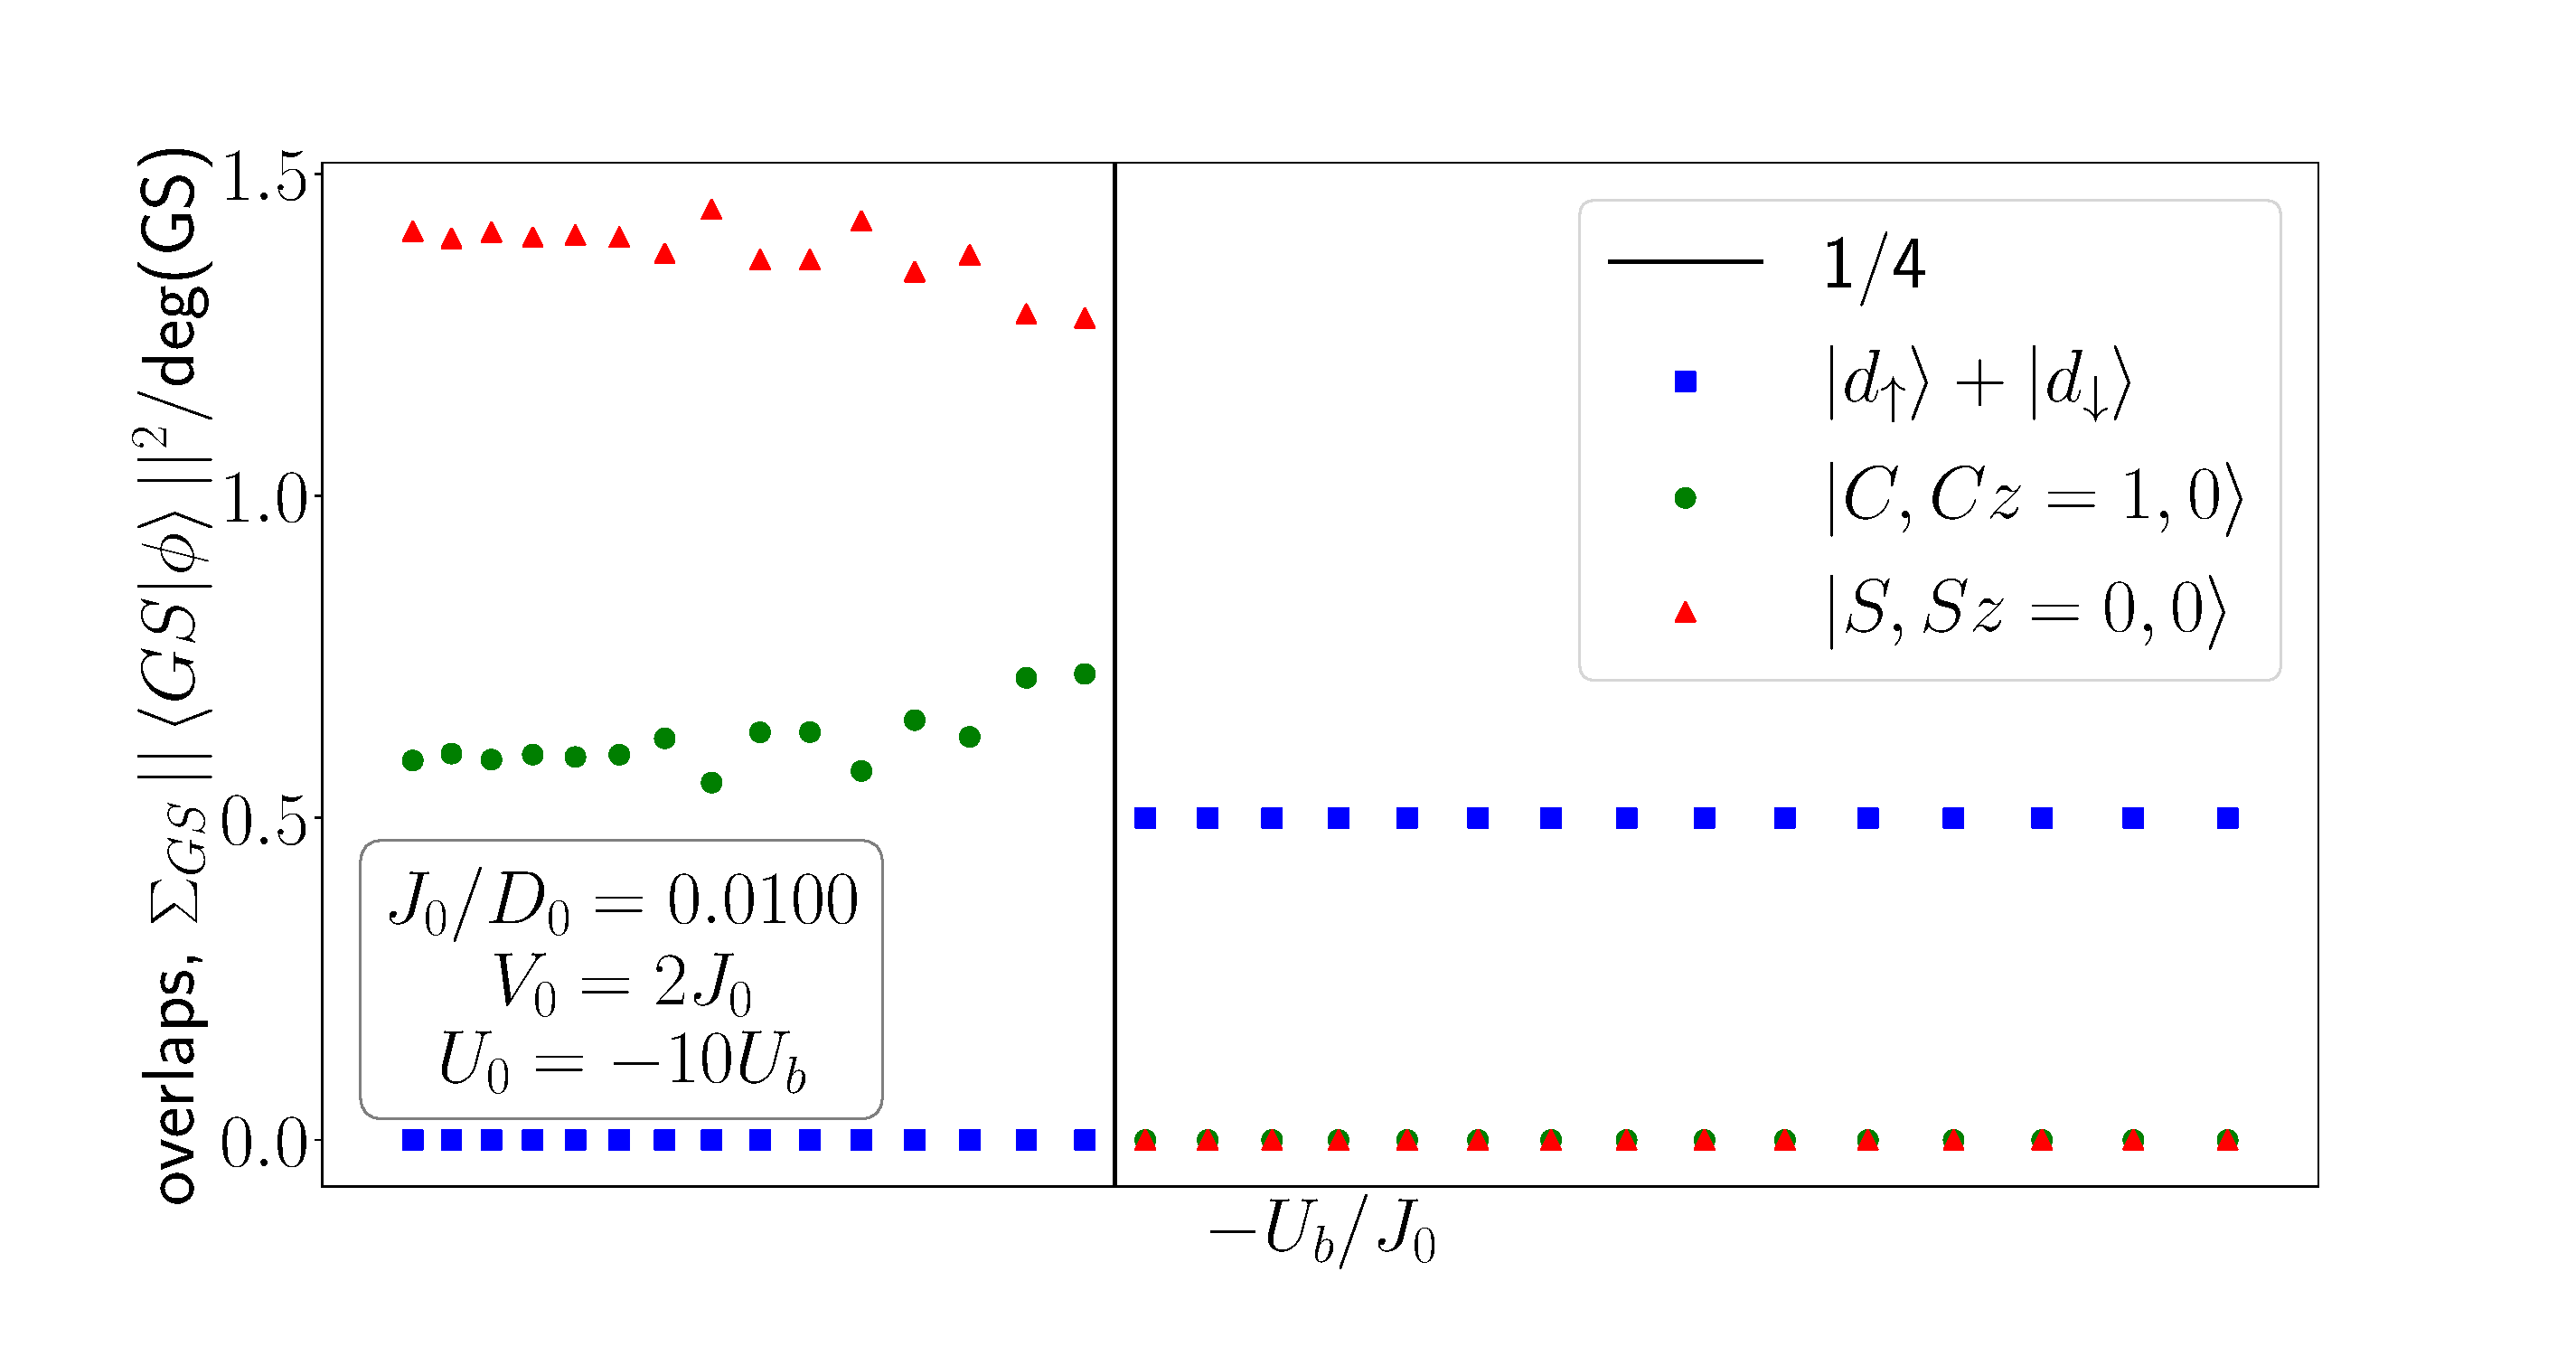
\includegraphics[width=\textwidth]{./figures/overlaps_gs-J=10.000.pdf}}

\only<3>{\(J_0/D_0 = 10^{-1}\)

\vspace*{-20pt}
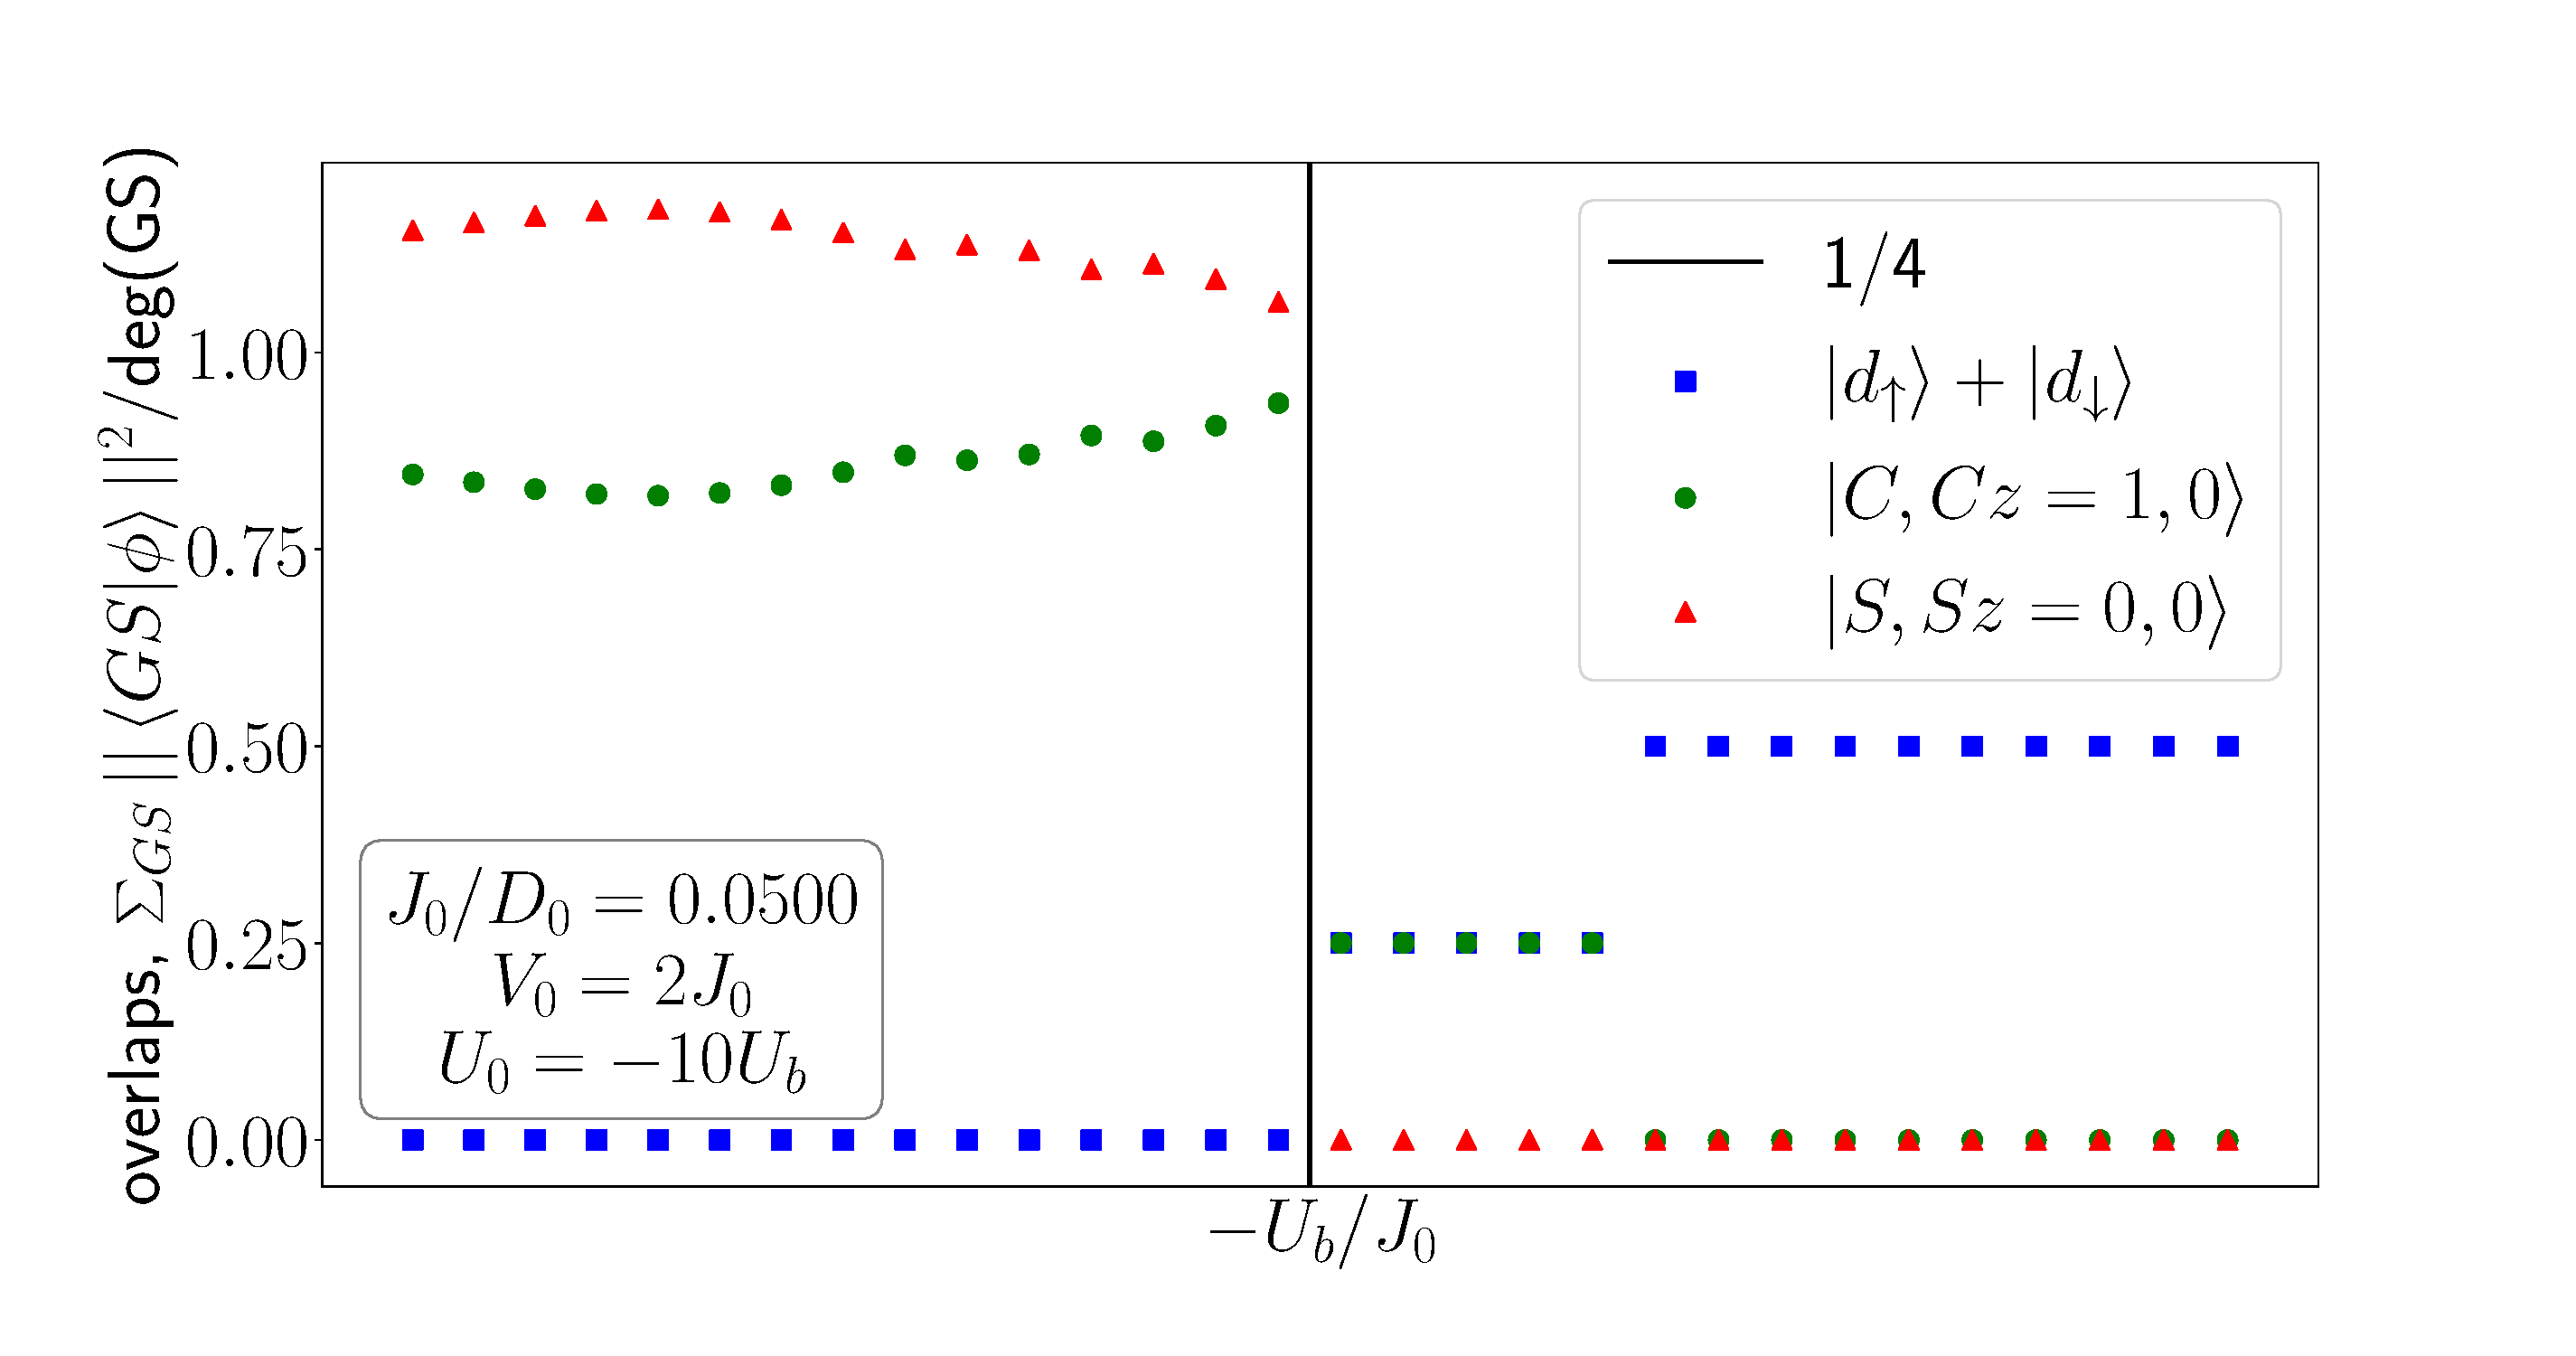
\includegraphics[width=\textwidth]{./figures/overlaps_gs-J=50.000.pdf}}

\end{frame}

\begin{frame}[noframenumbering]{Spin and charge correlations in ground state}
	\centering
\only<1>{\(J_0/D_0 = 10^{-4}\)

\vspace*{-20pt}
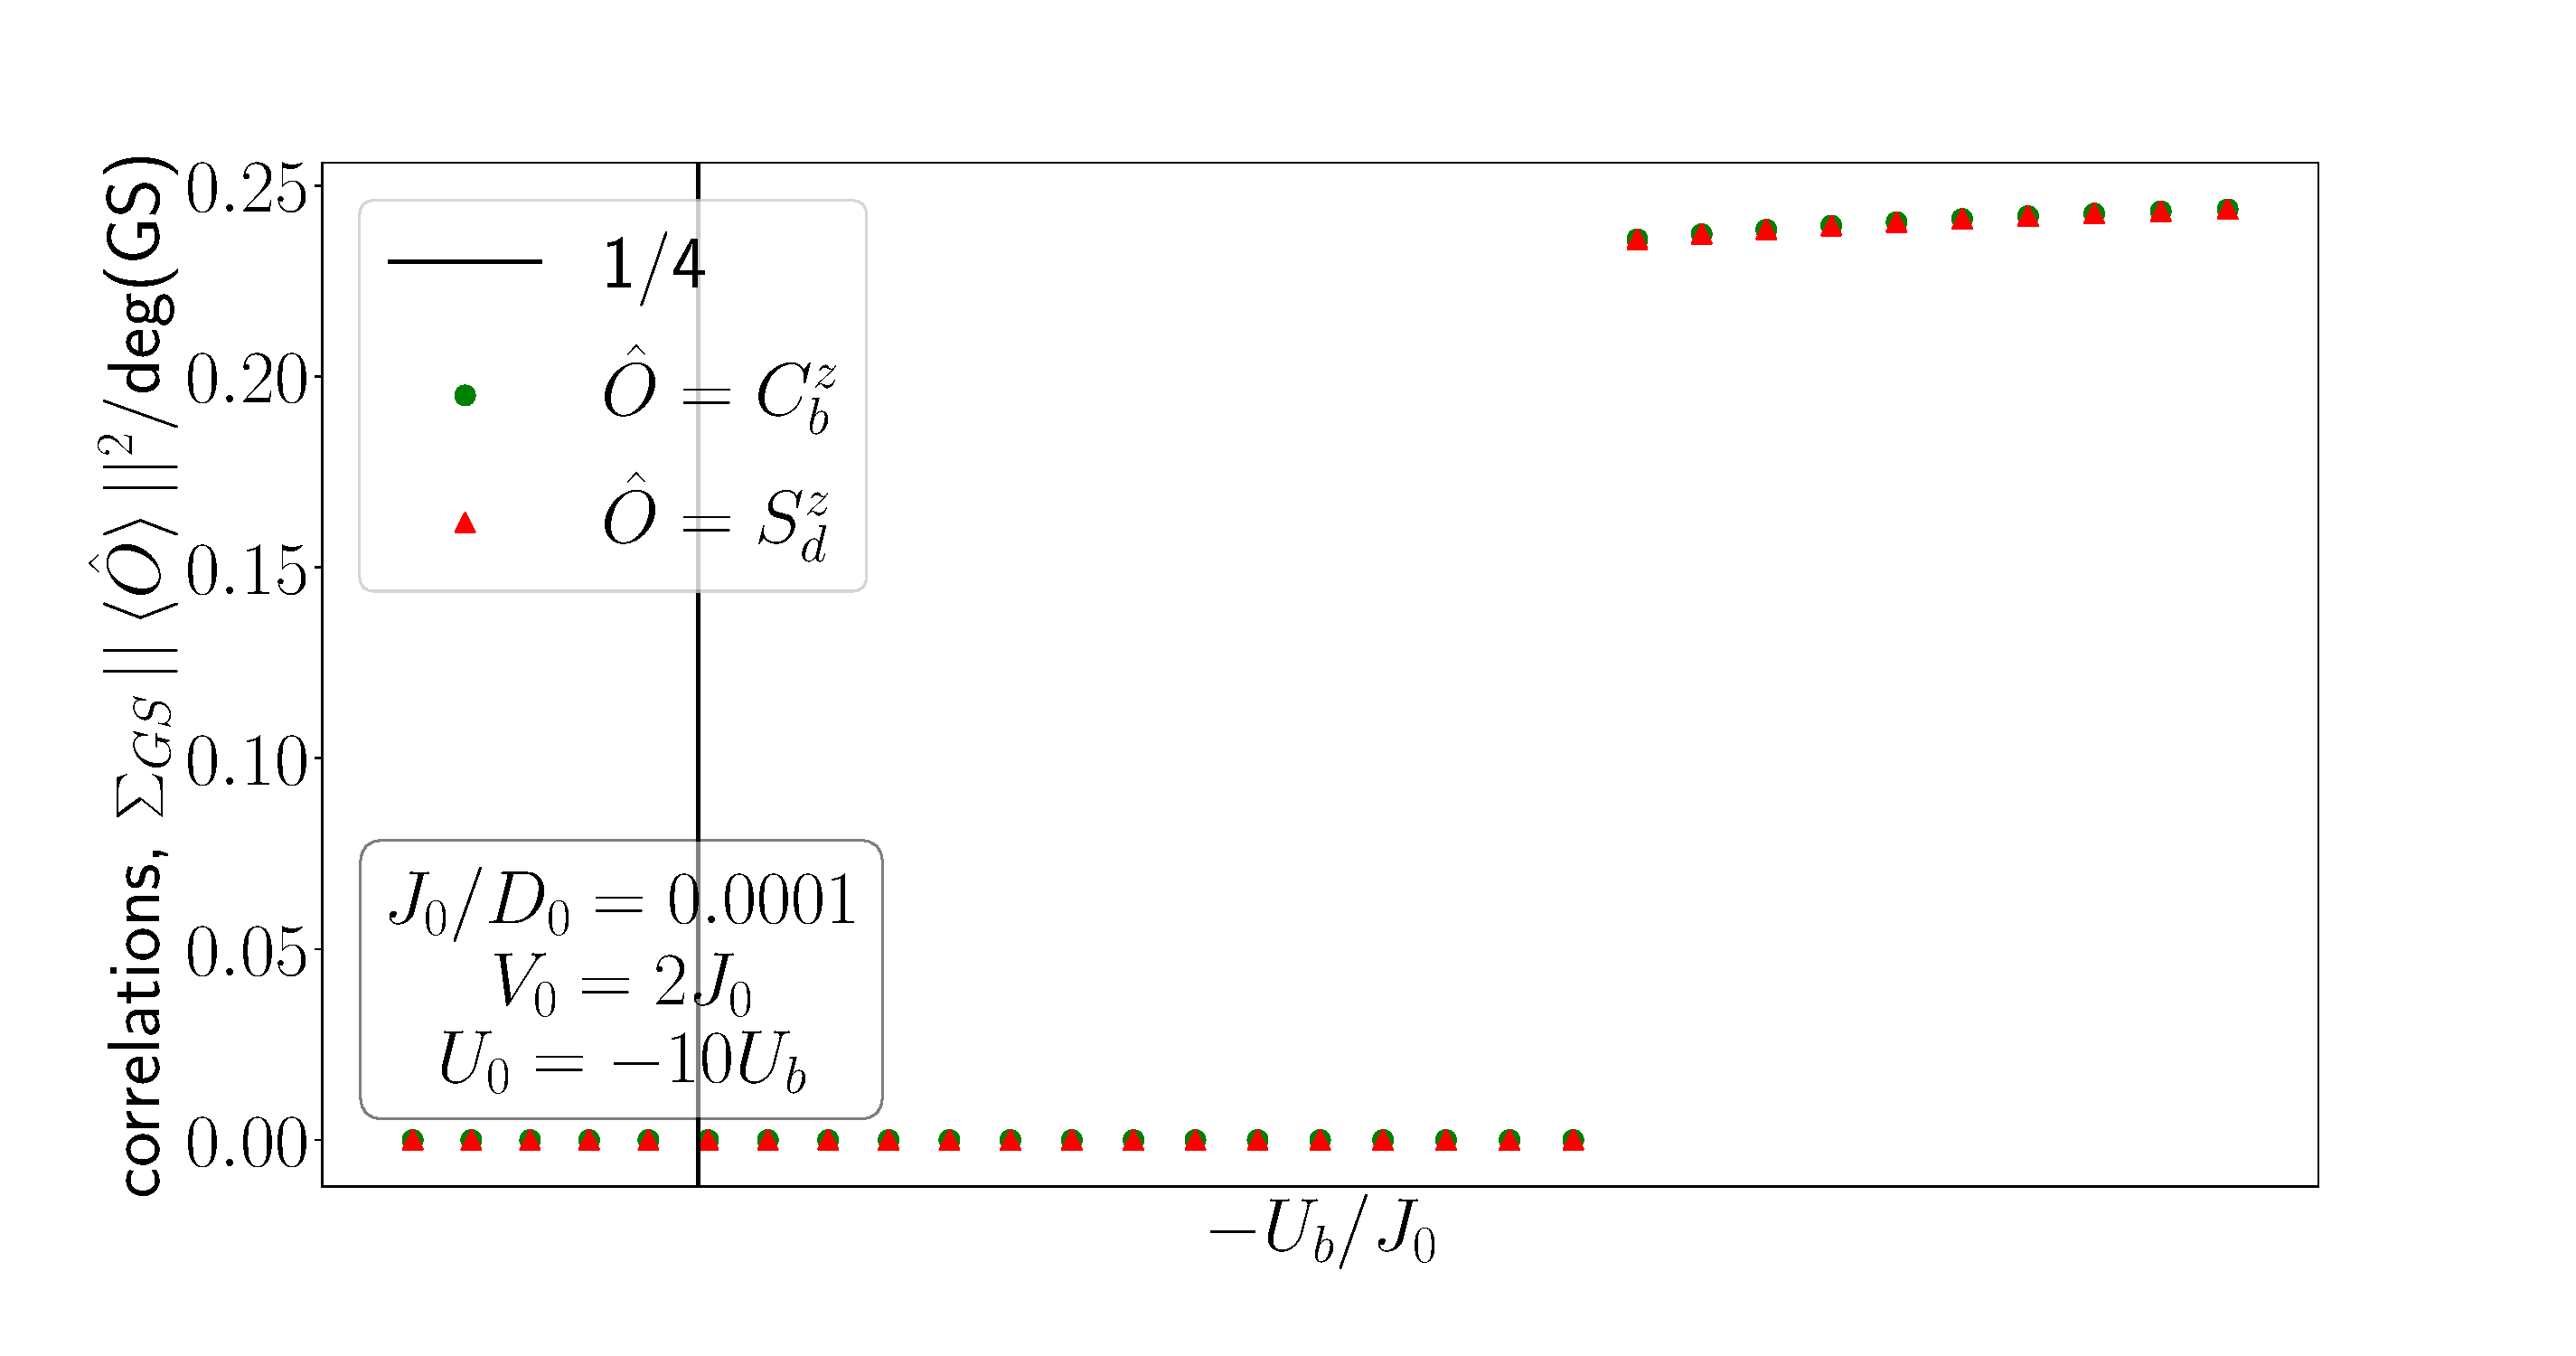
\includegraphics[width=\textwidth]{./figures/corrs_gs-J=0.100.pdf}
}

\only<2>{\(J_0/D_0 = 10^{-2}\)

\vspace*{-20pt}
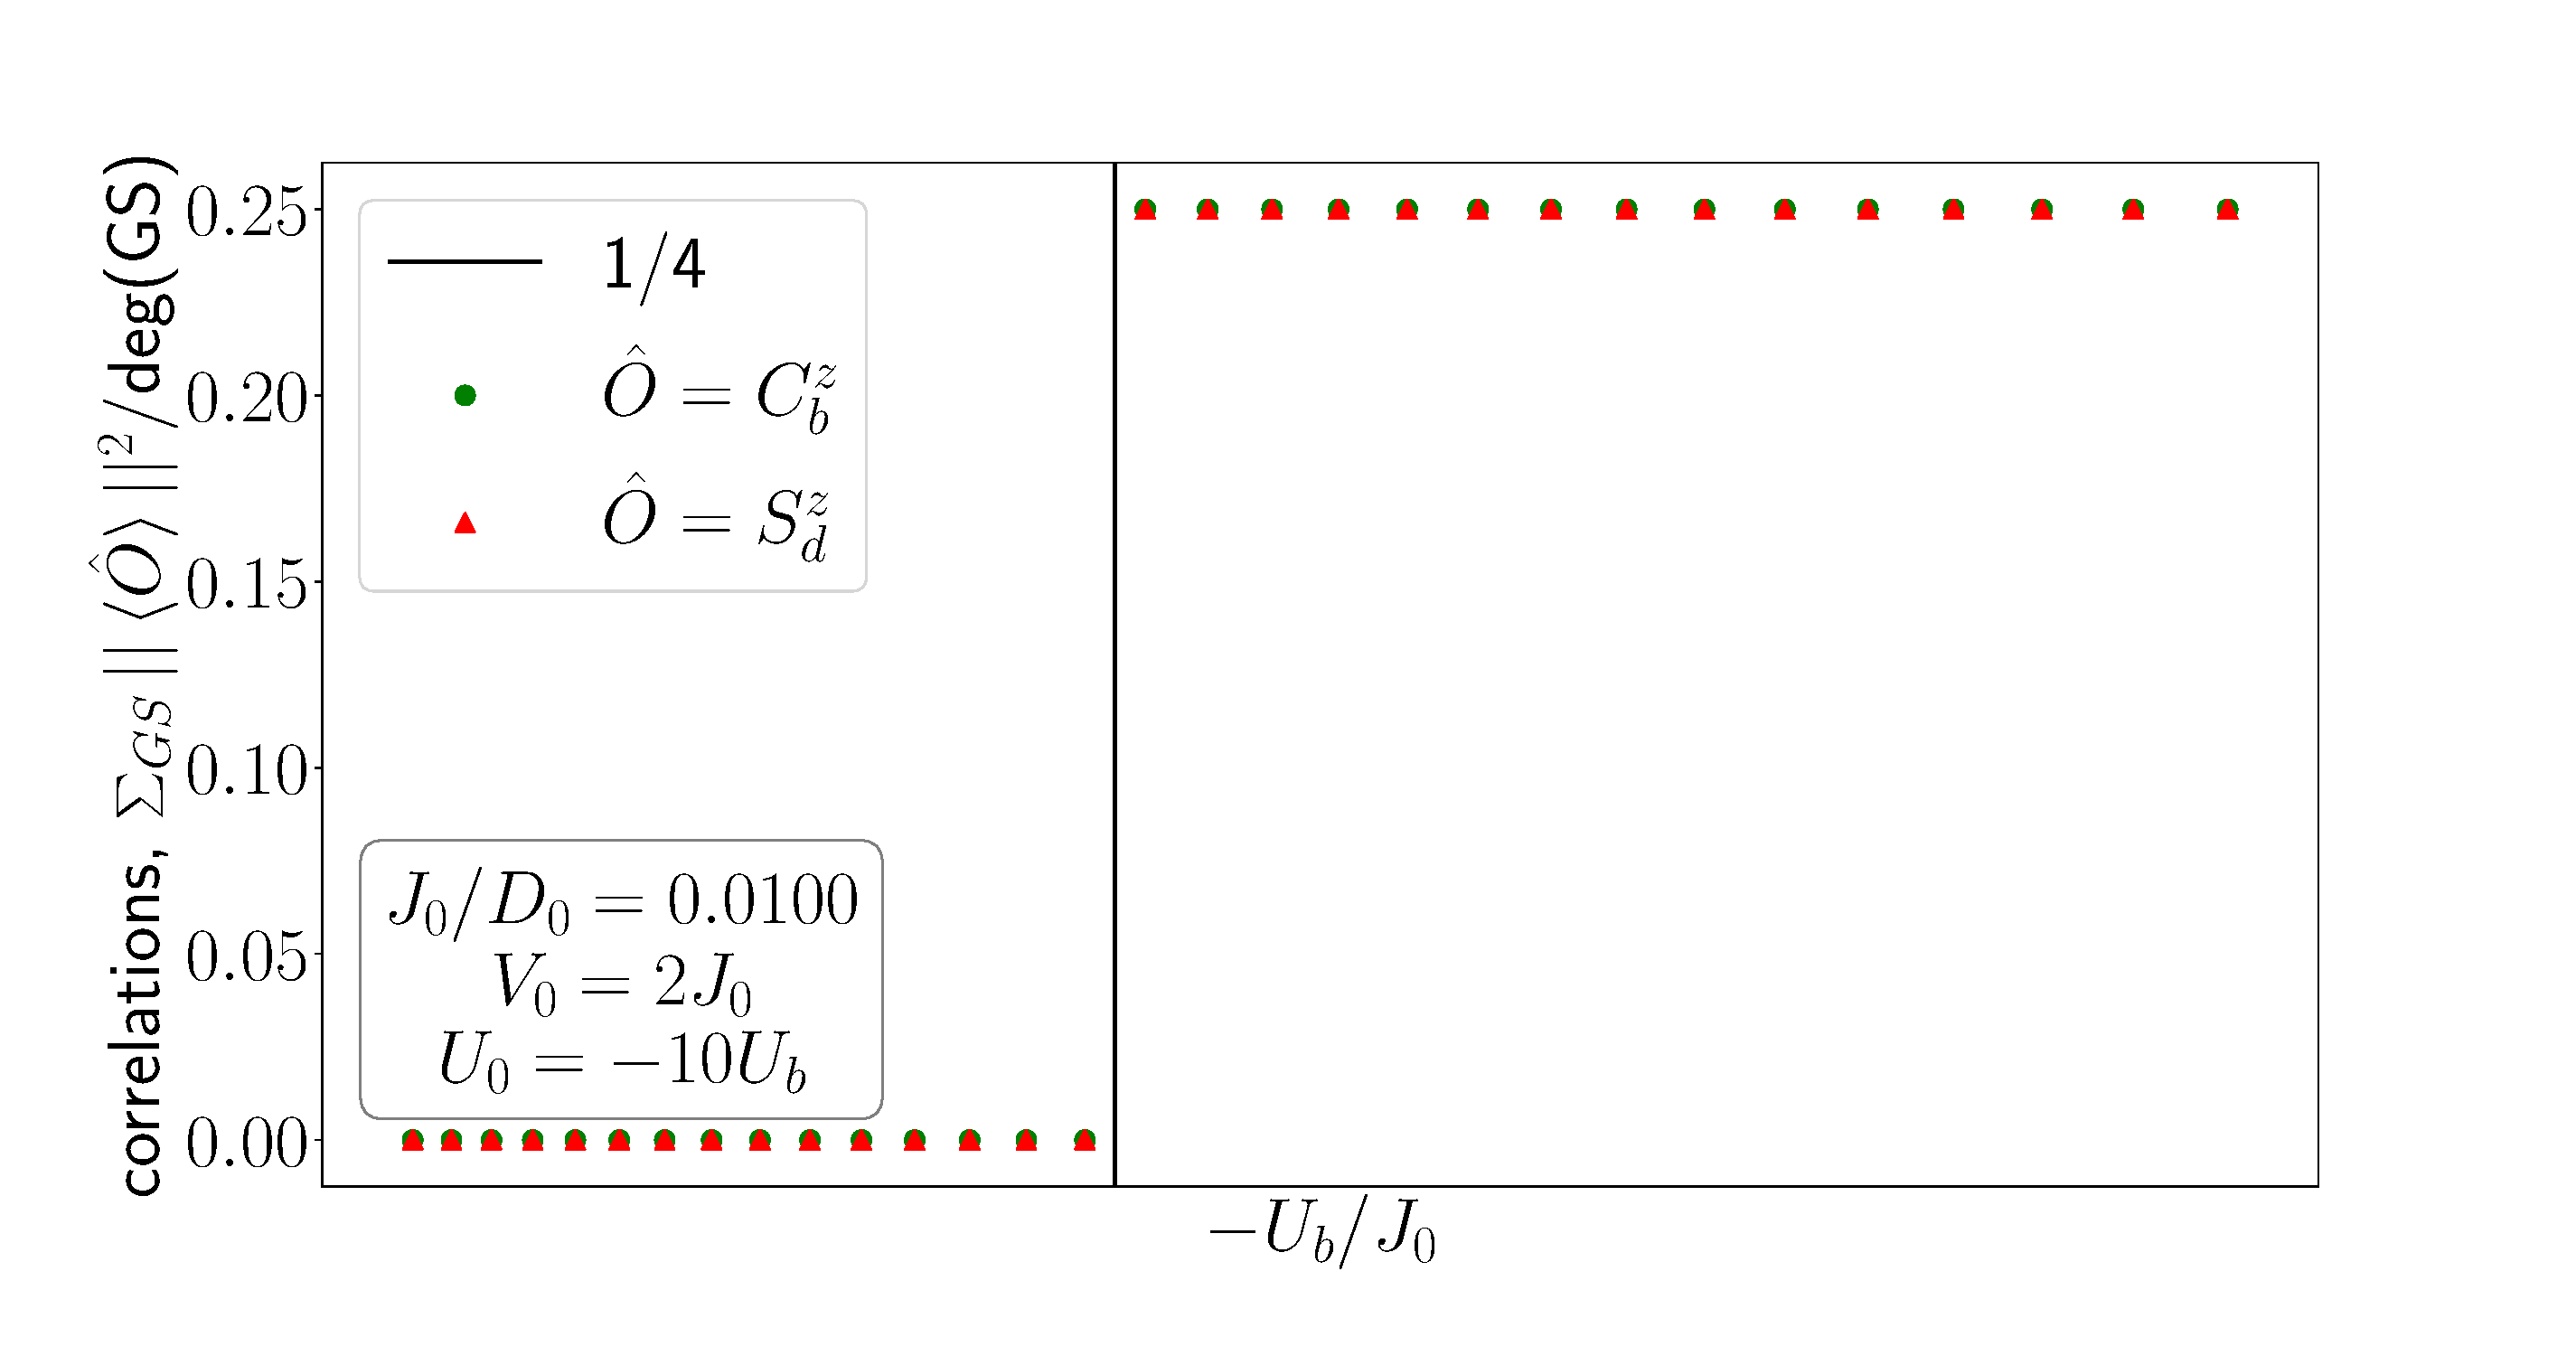
\includegraphics[width=\textwidth]{./figures/corrs_gs-J=10.000.pdf}}

\only<3>{\(J_0/D_0 = 10^{-1}\)

\vspace*{-20pt}
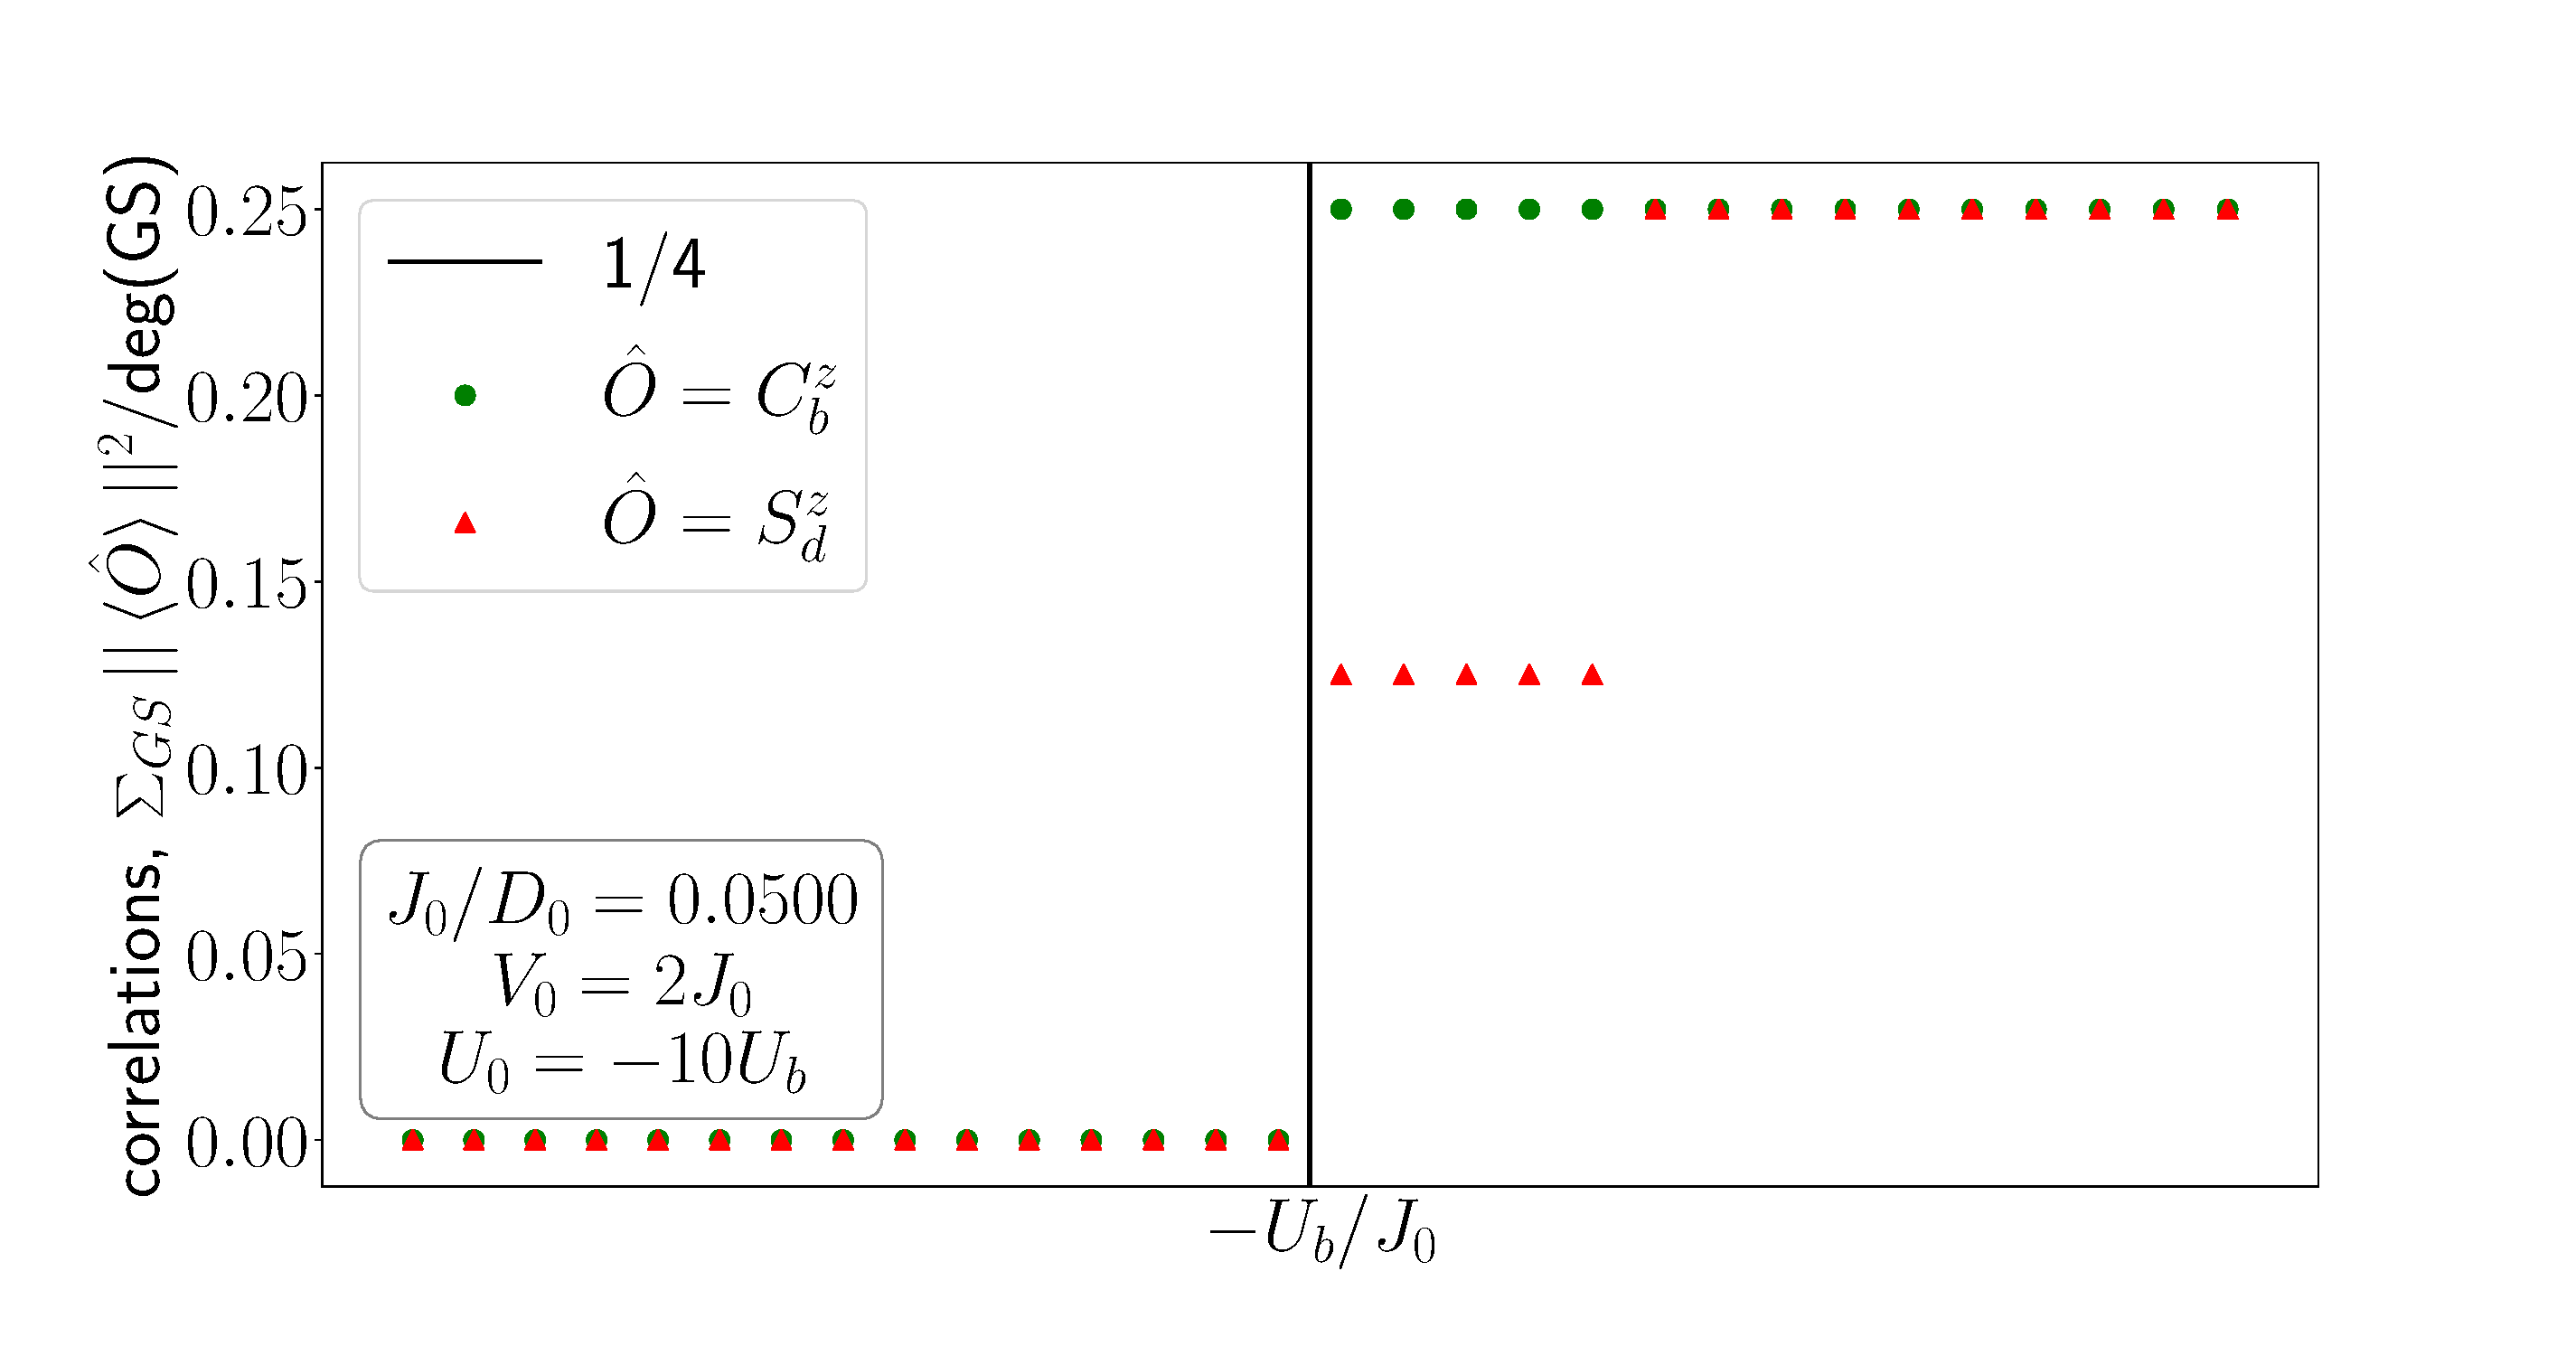
\includegraphics[width=\textwidth]{./figures/corrs_gs-J=50.000.pdf}}

\end{frame}

\begin{frame}[noframenumbering]{Correlation measures: Local Fermi liquid}
\vspace*{20pt}
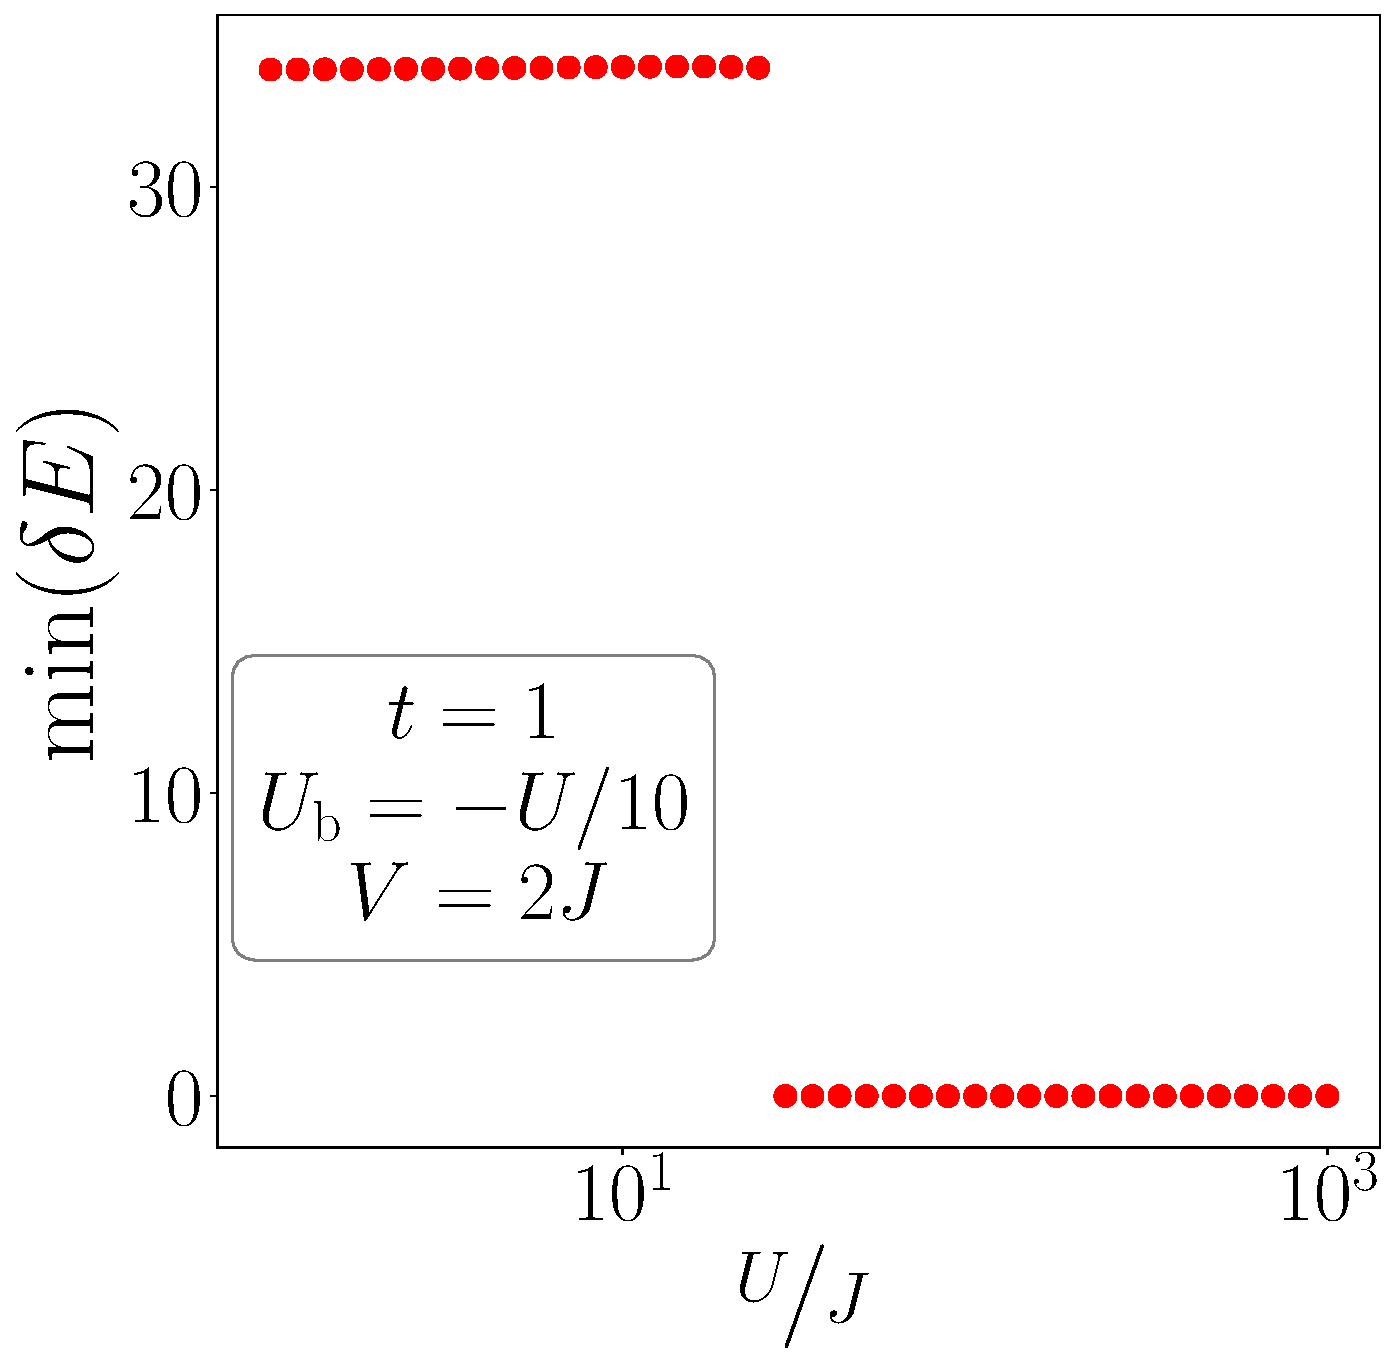
\includegraphics[width=0.49\textwidth]{./figures/gap-t=1.000,J=10.000,0.000,40,V=3J,Ubath=-U_by_10,N=4,U=1.000,1000.000,40.pdf}
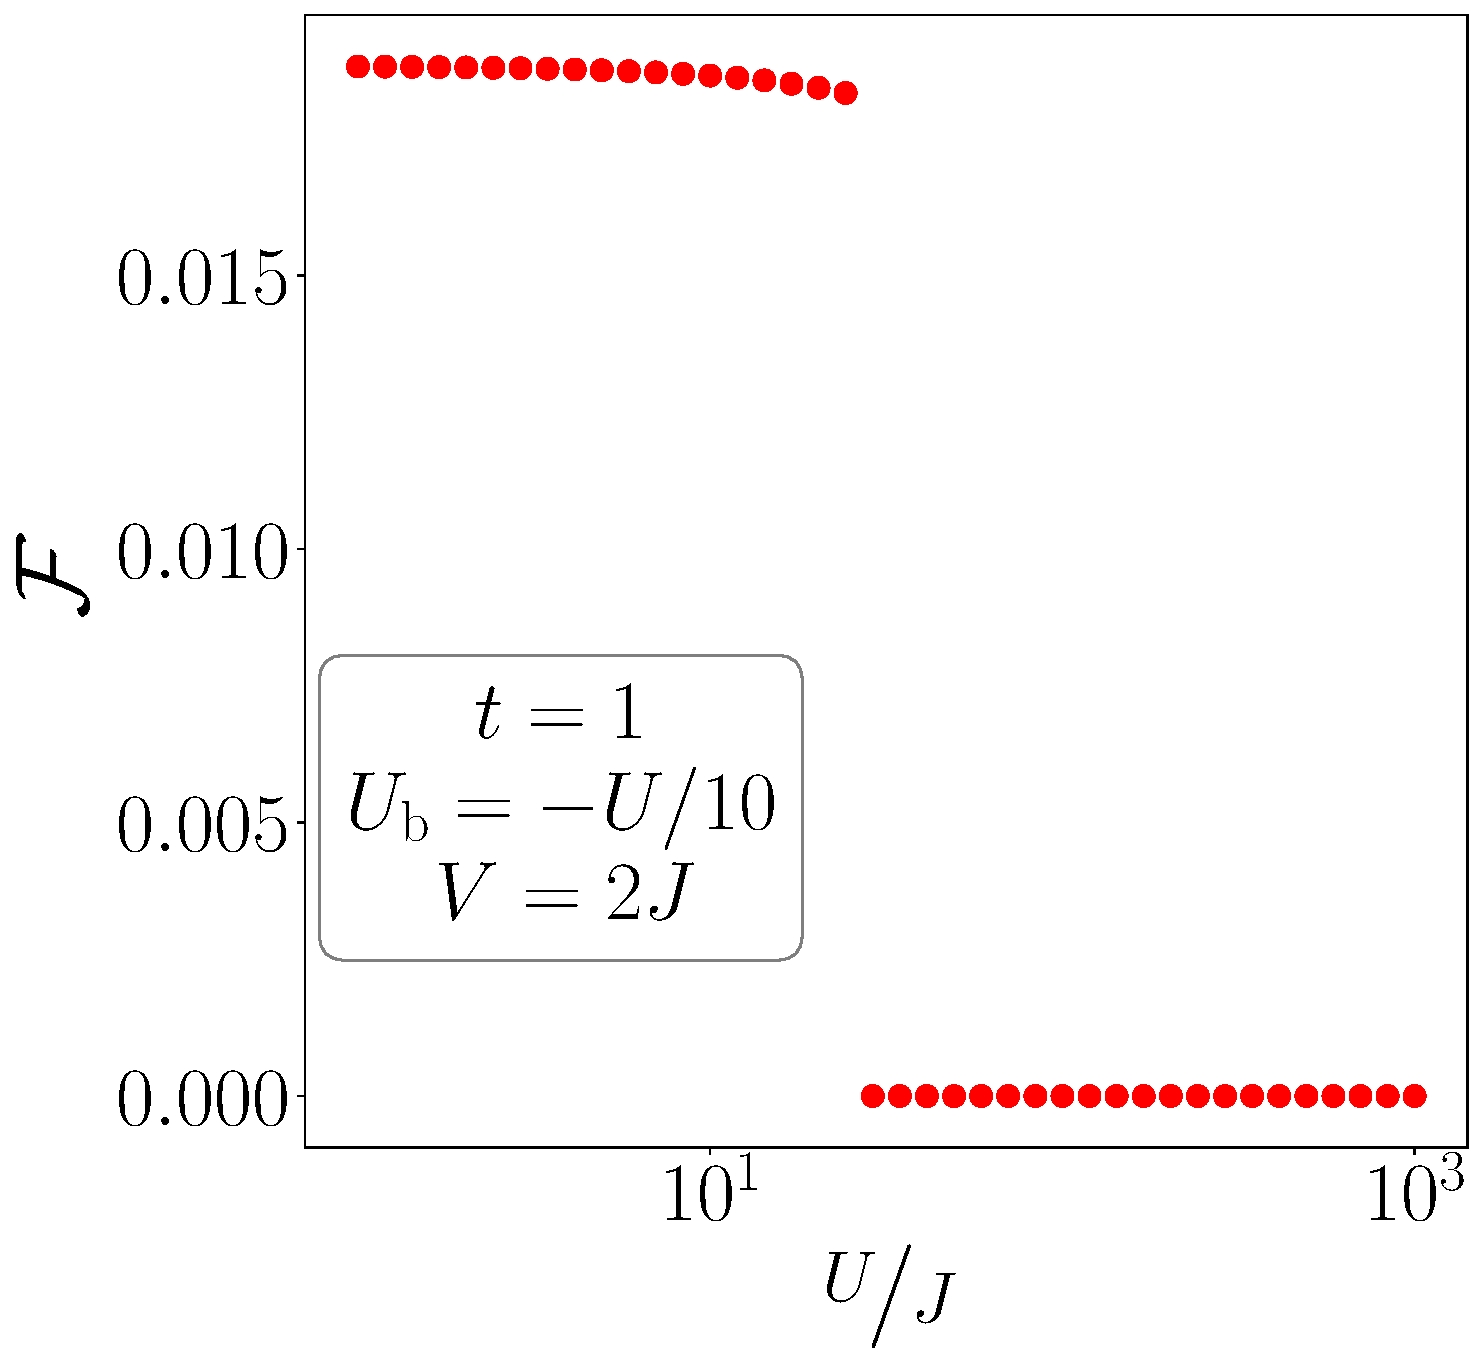
\includegraphics[width=0.49\textwidth]{./figures/lfl-t=1.000,J=10.000,0.000,40,V=3J,Ubath=-U_by_10,N=4,U=1.000,1000.000,40.pdf}
\end{frame}


\begin{frame}[noframenumbering]{Correlation measures: Kondo cloud}
\vspace*{20pt}
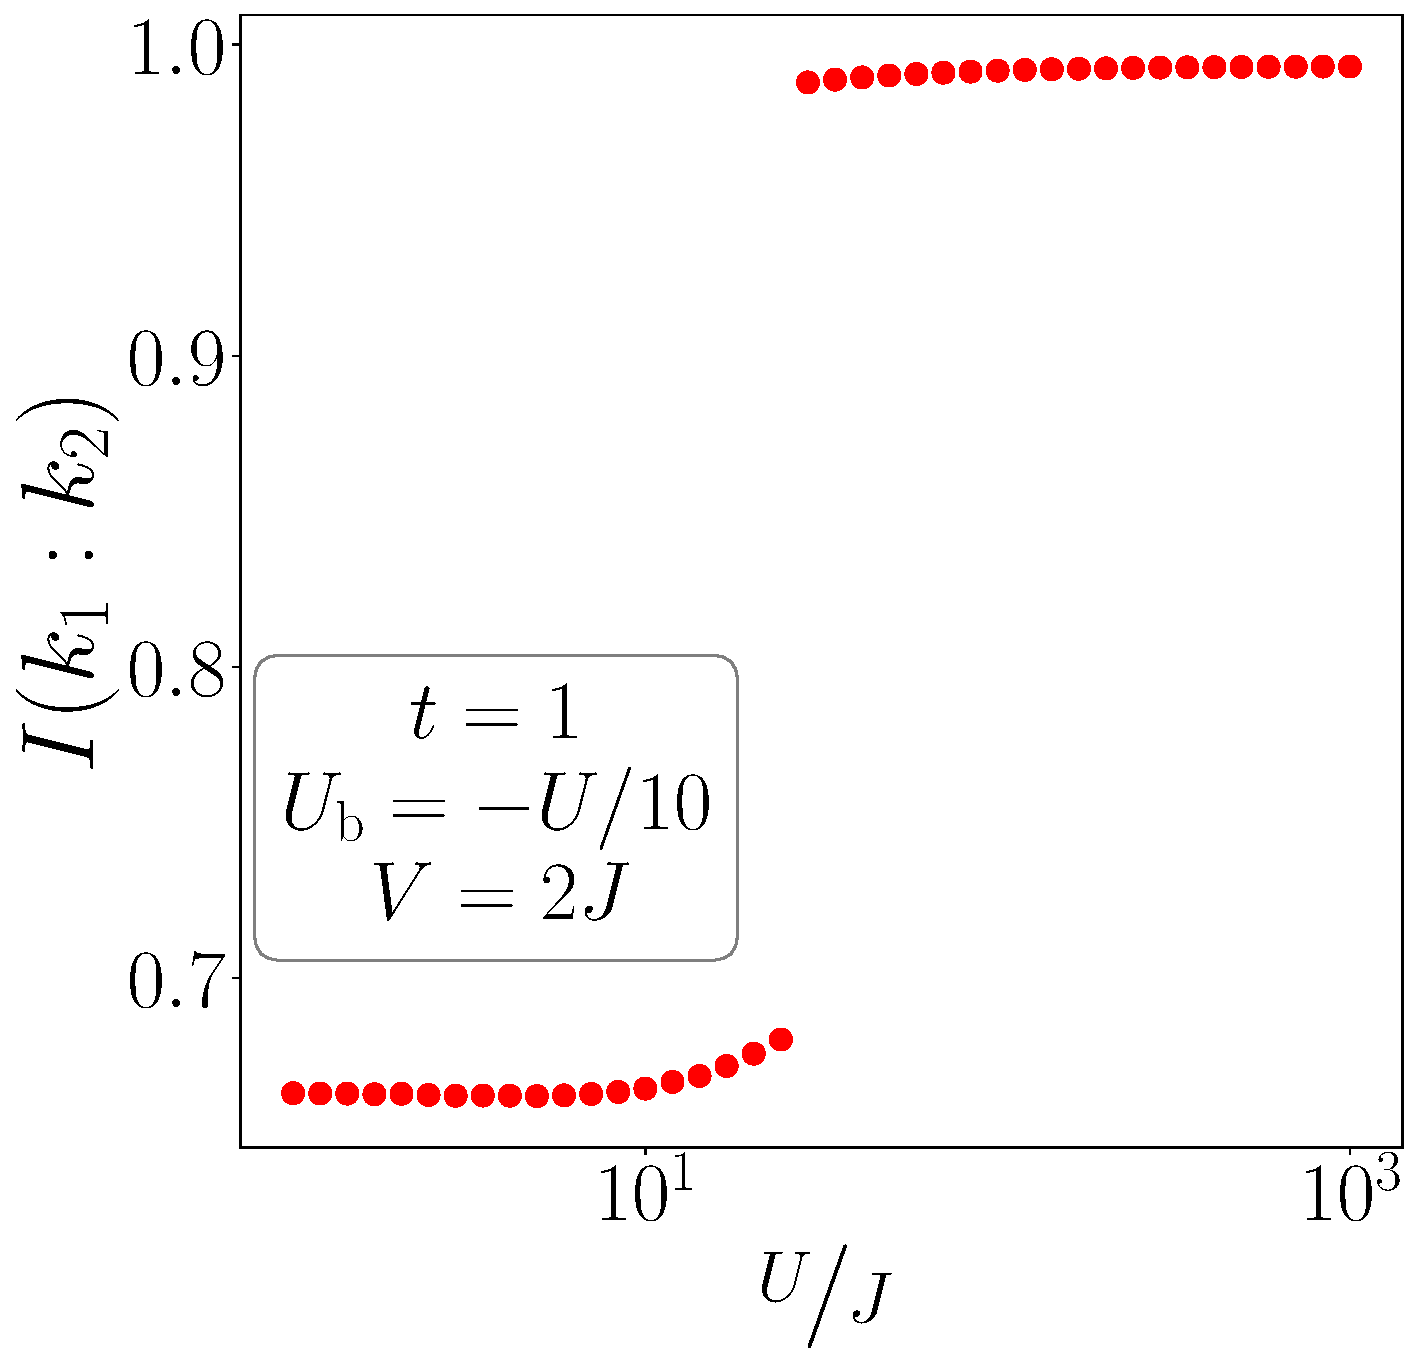
\includegraphics[width=0.49\textwidth]{./figures/corr-k-t=1.000,J=10.000,0.000,40,V=3J,Ubath=-U_by_10,N=4,U=1.000,1000.000,40.pdf}
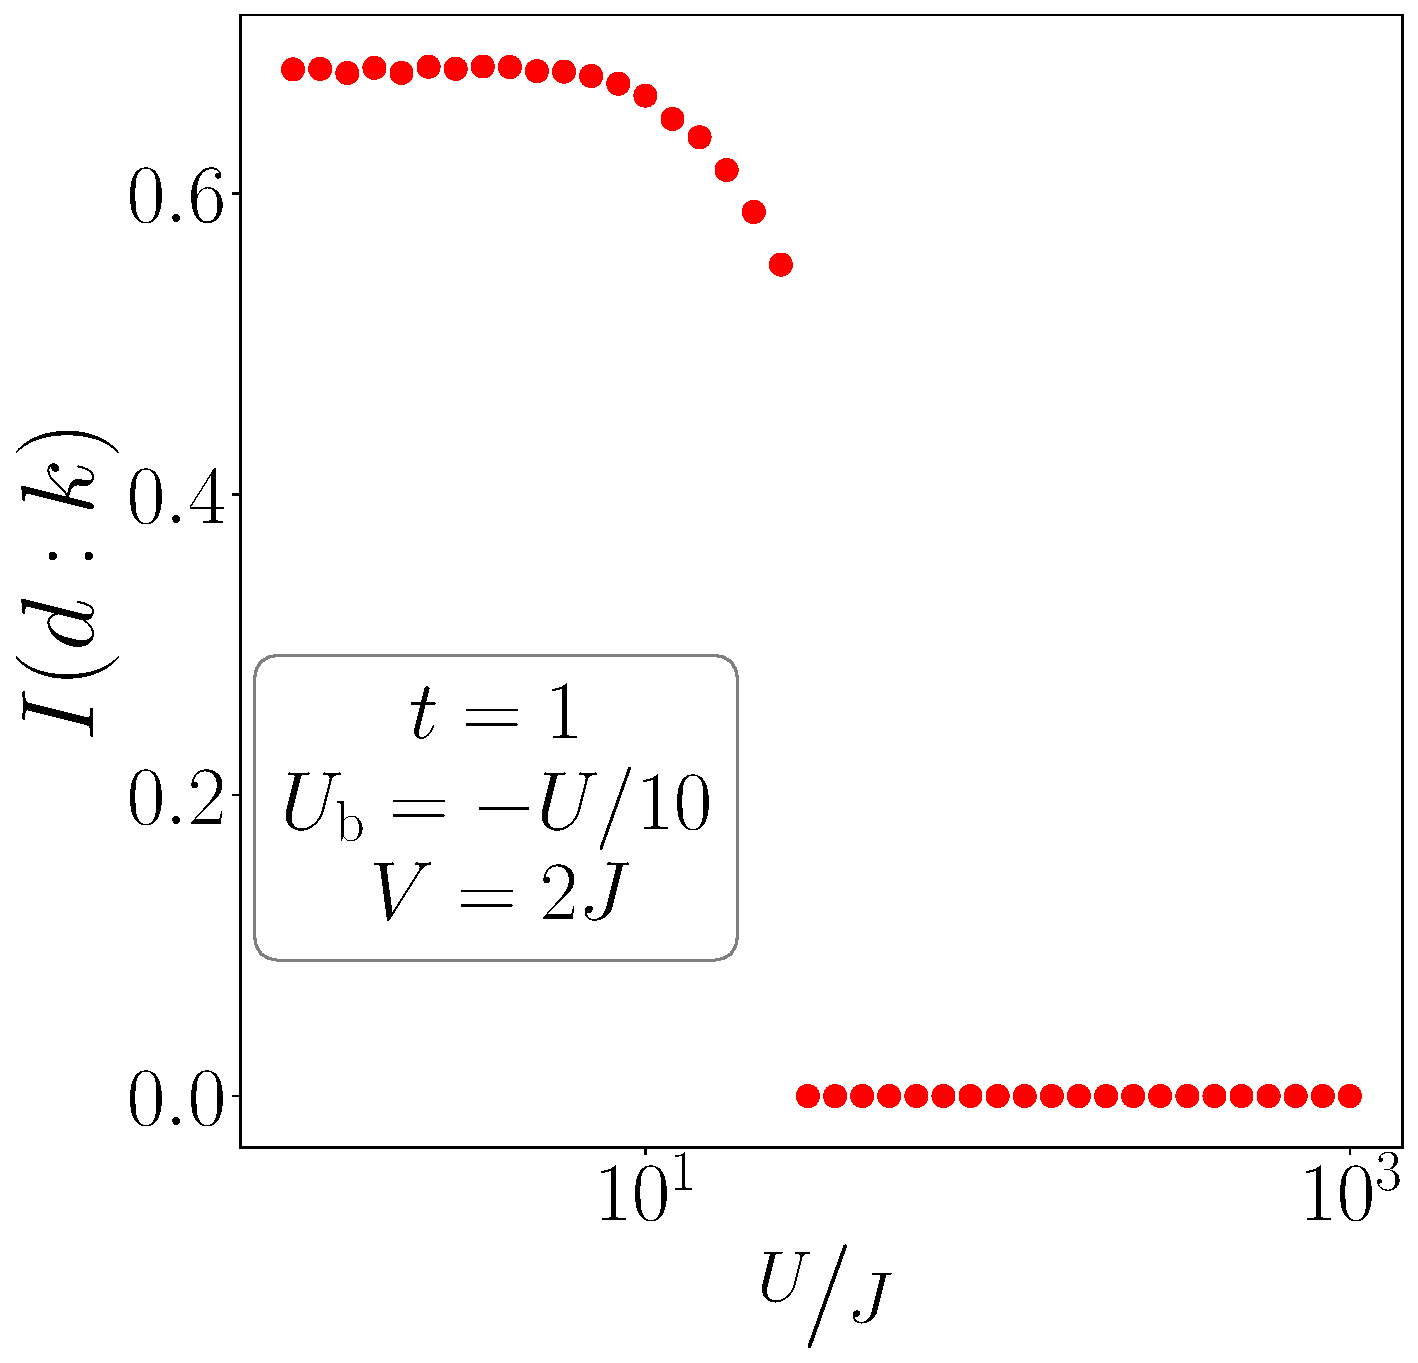
\includegraphics[width=0.49\textwidth]{./figures/mi-dk-t=1.000,J=10.000,0.000,40,V=3J,Ubath=-U_by_10,N=4,U=1.000,1000.000,40.pdf}
\end{frame}

\begin{frame}[noframenumbering]{Correlation measures: Real space mutual information}
\vspace*{20pt}
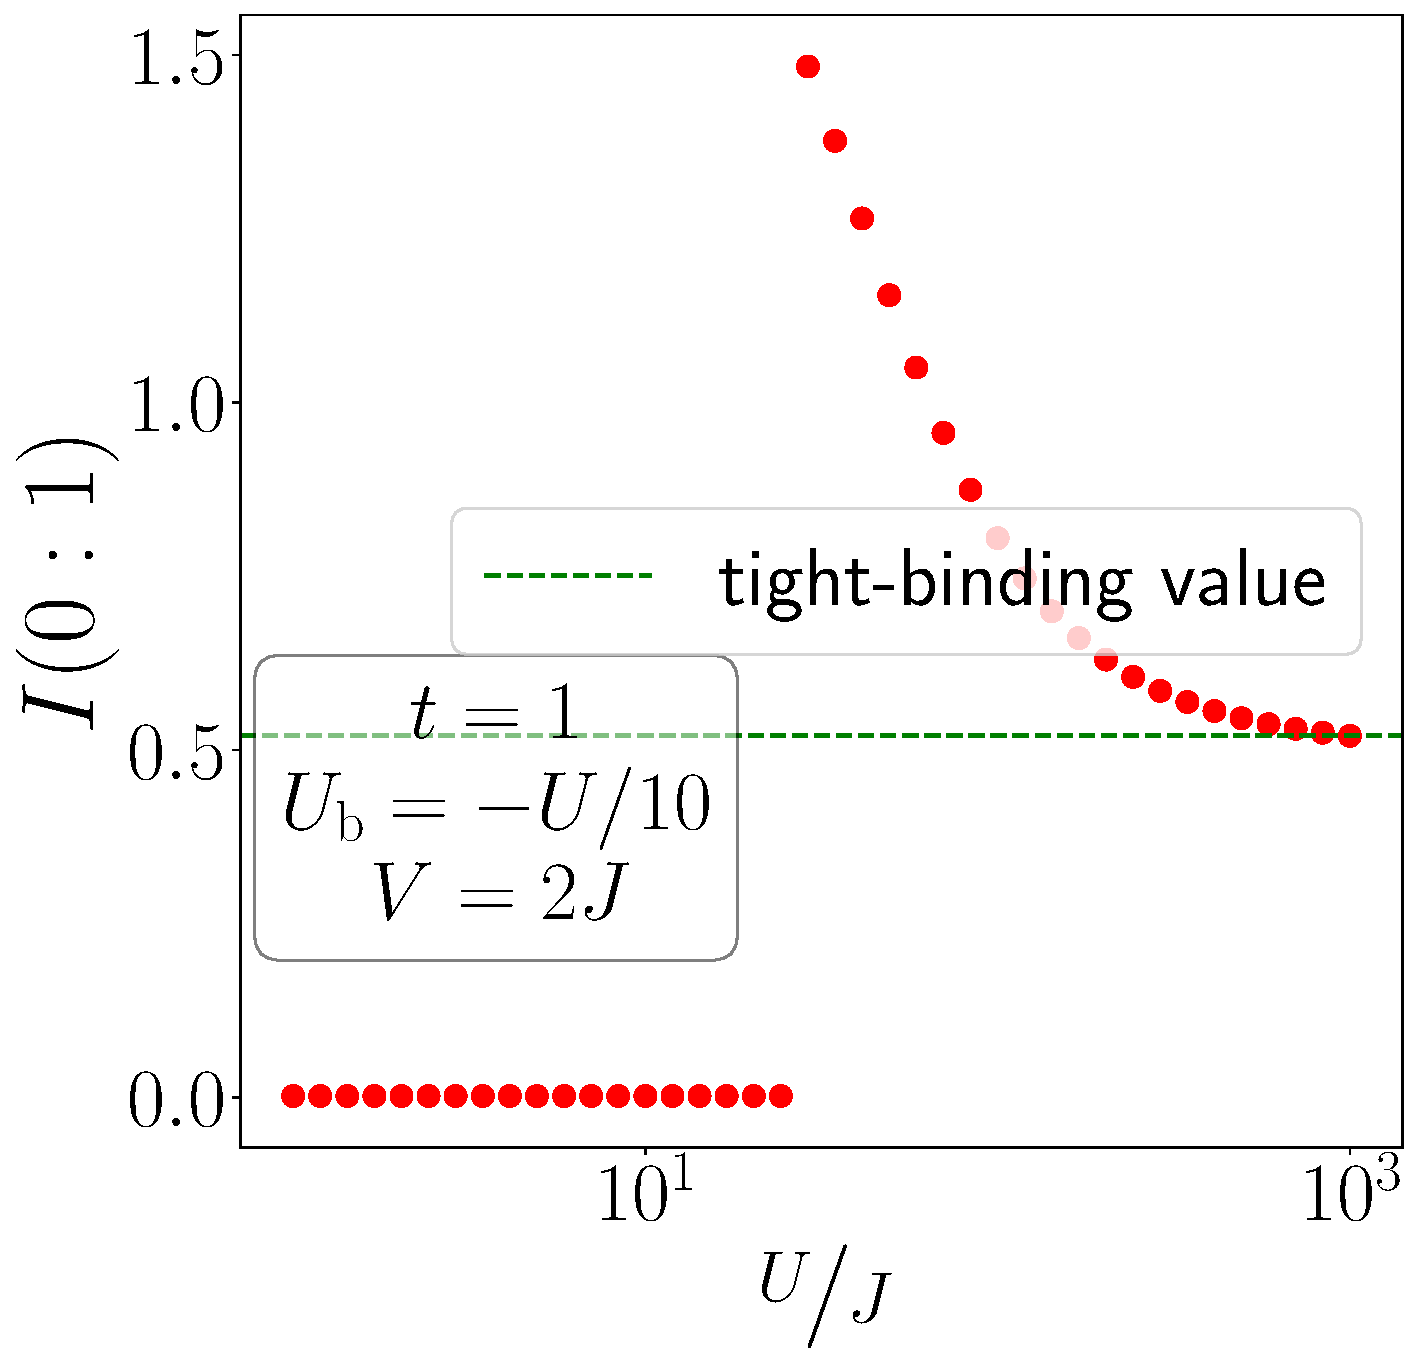
\includegraphics[width=0.49\textwidth]{./figures/mi-01-t=1.000,J=10.000,0.000,40,V=3J,Ubath=-U_by_10,N=4,U=1.000,1000.000,40.pdf}
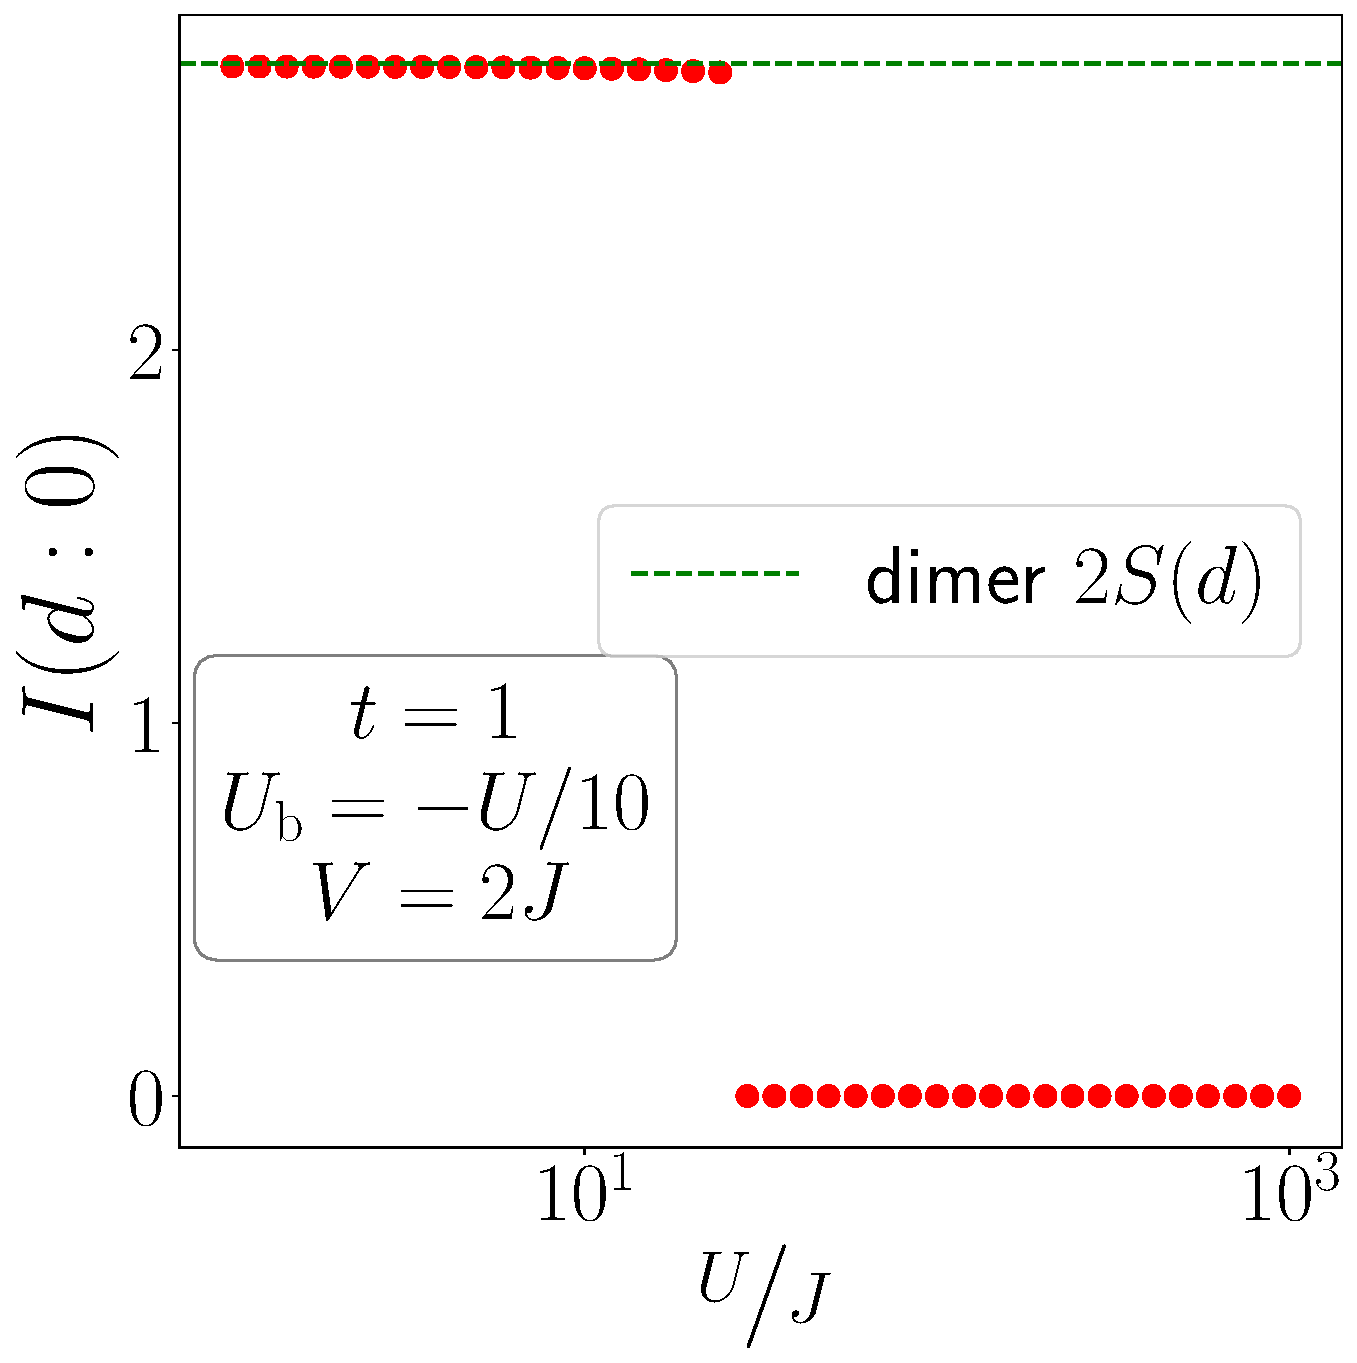
\includegraphics[width=0.49\textwidth]{./figures/mi-d0-t=1.000,J=10.000,0.000,40,V=3J,Ubath=-U_by_10,N=4,U=1.000,1000.000,40.pdf}
\end{frame}


\begin{frame}[noframenumbering]{Correlation measures: Impurity entanglement entropy and spin-spin correlations}
\vspace*{20pt}
	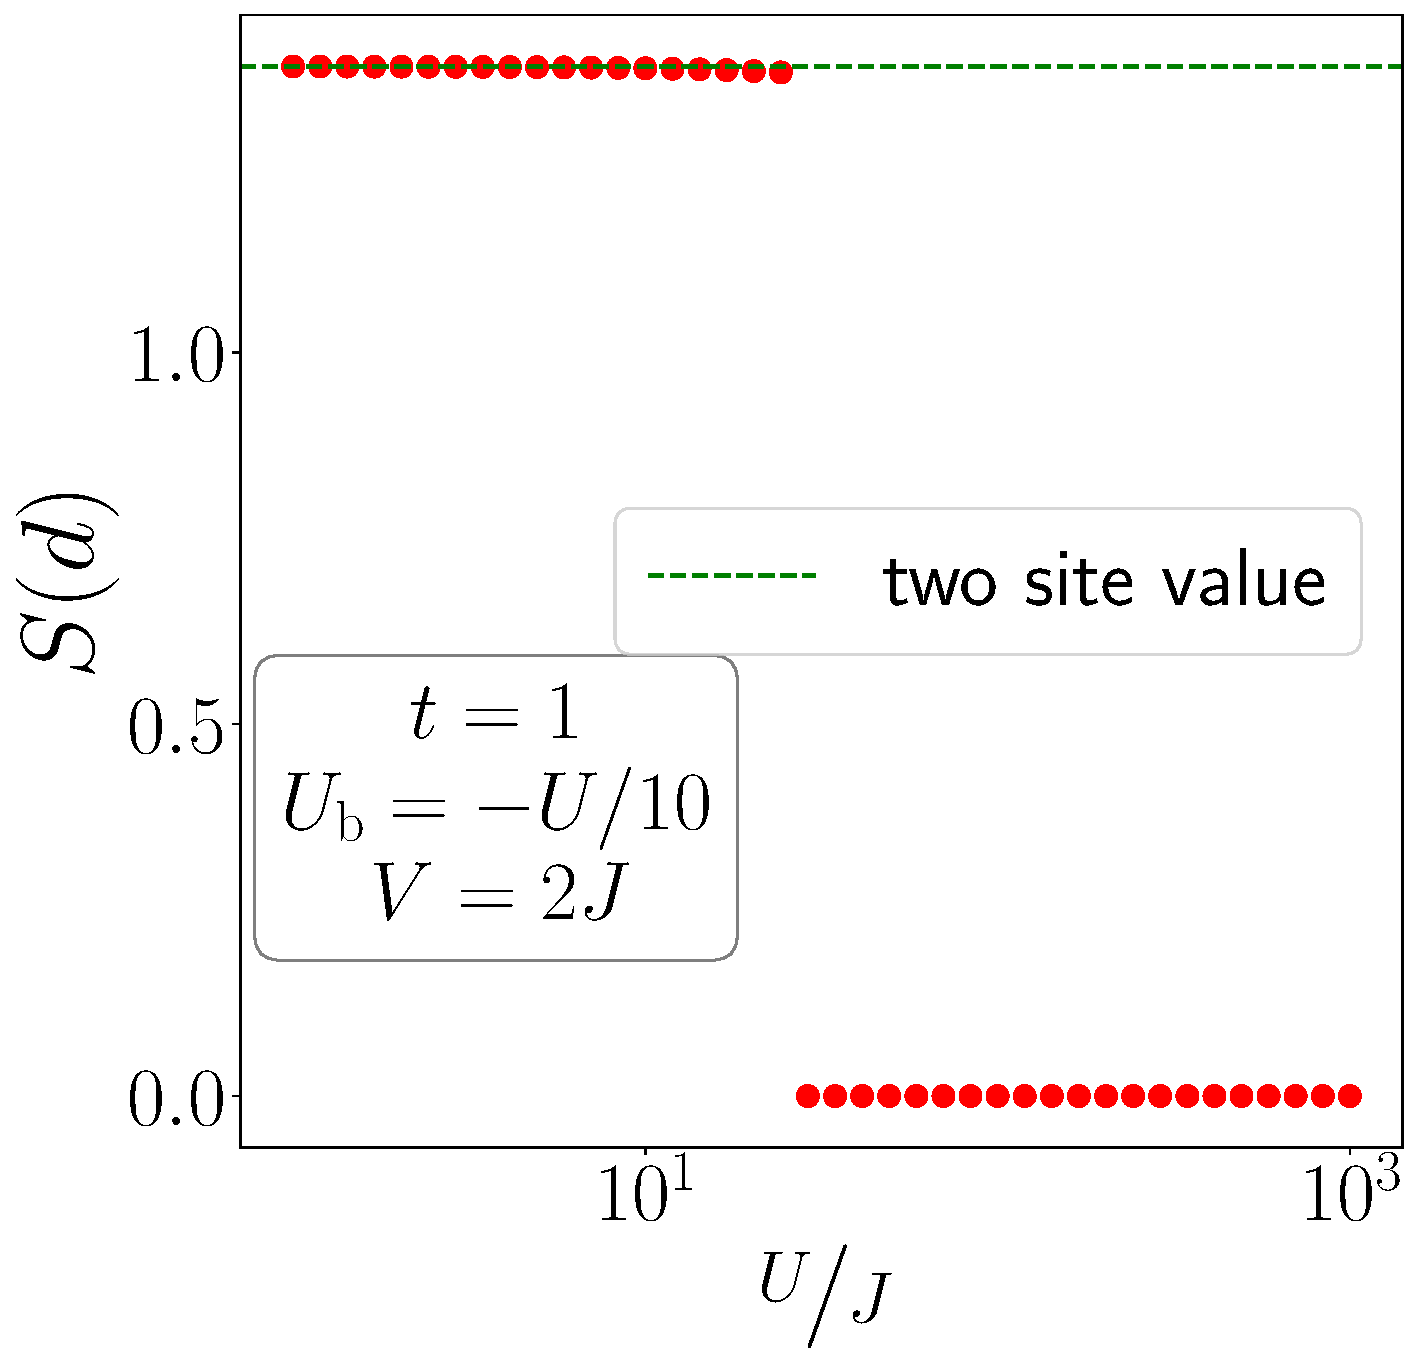
\includegraphics[width=0.32\textwidth]{./figures/EE-d-t=1.000,J=10.000,0.000,40,V=3J,Ubath=-U_by_10,N=4,U=1.000,1000.000,40.pdf}
	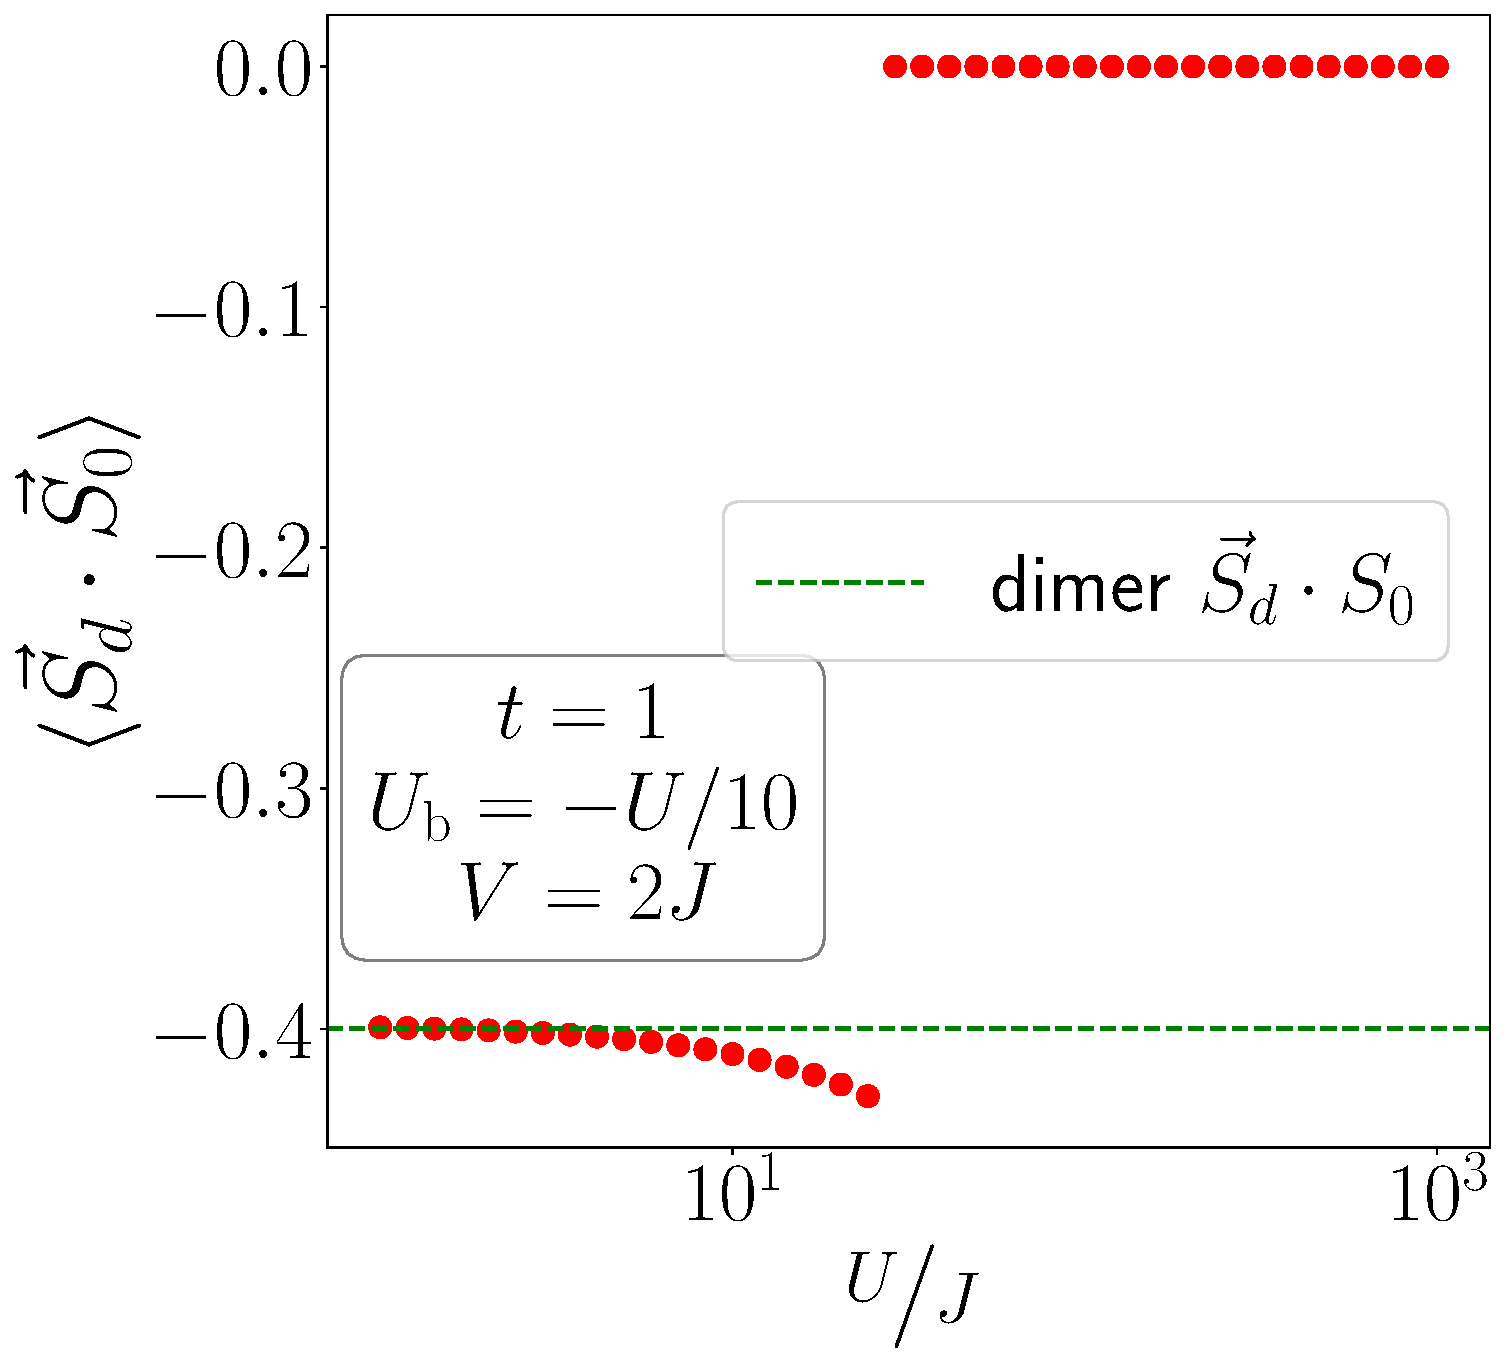
\includegraphics[width=0.32\textwidth]{./figures/corr-d0-t=1.000,J=10.000,0.000,40,V=3J,Ubath=-U_by_10,N=4,U=1.000,1000.000,40.pdf}
	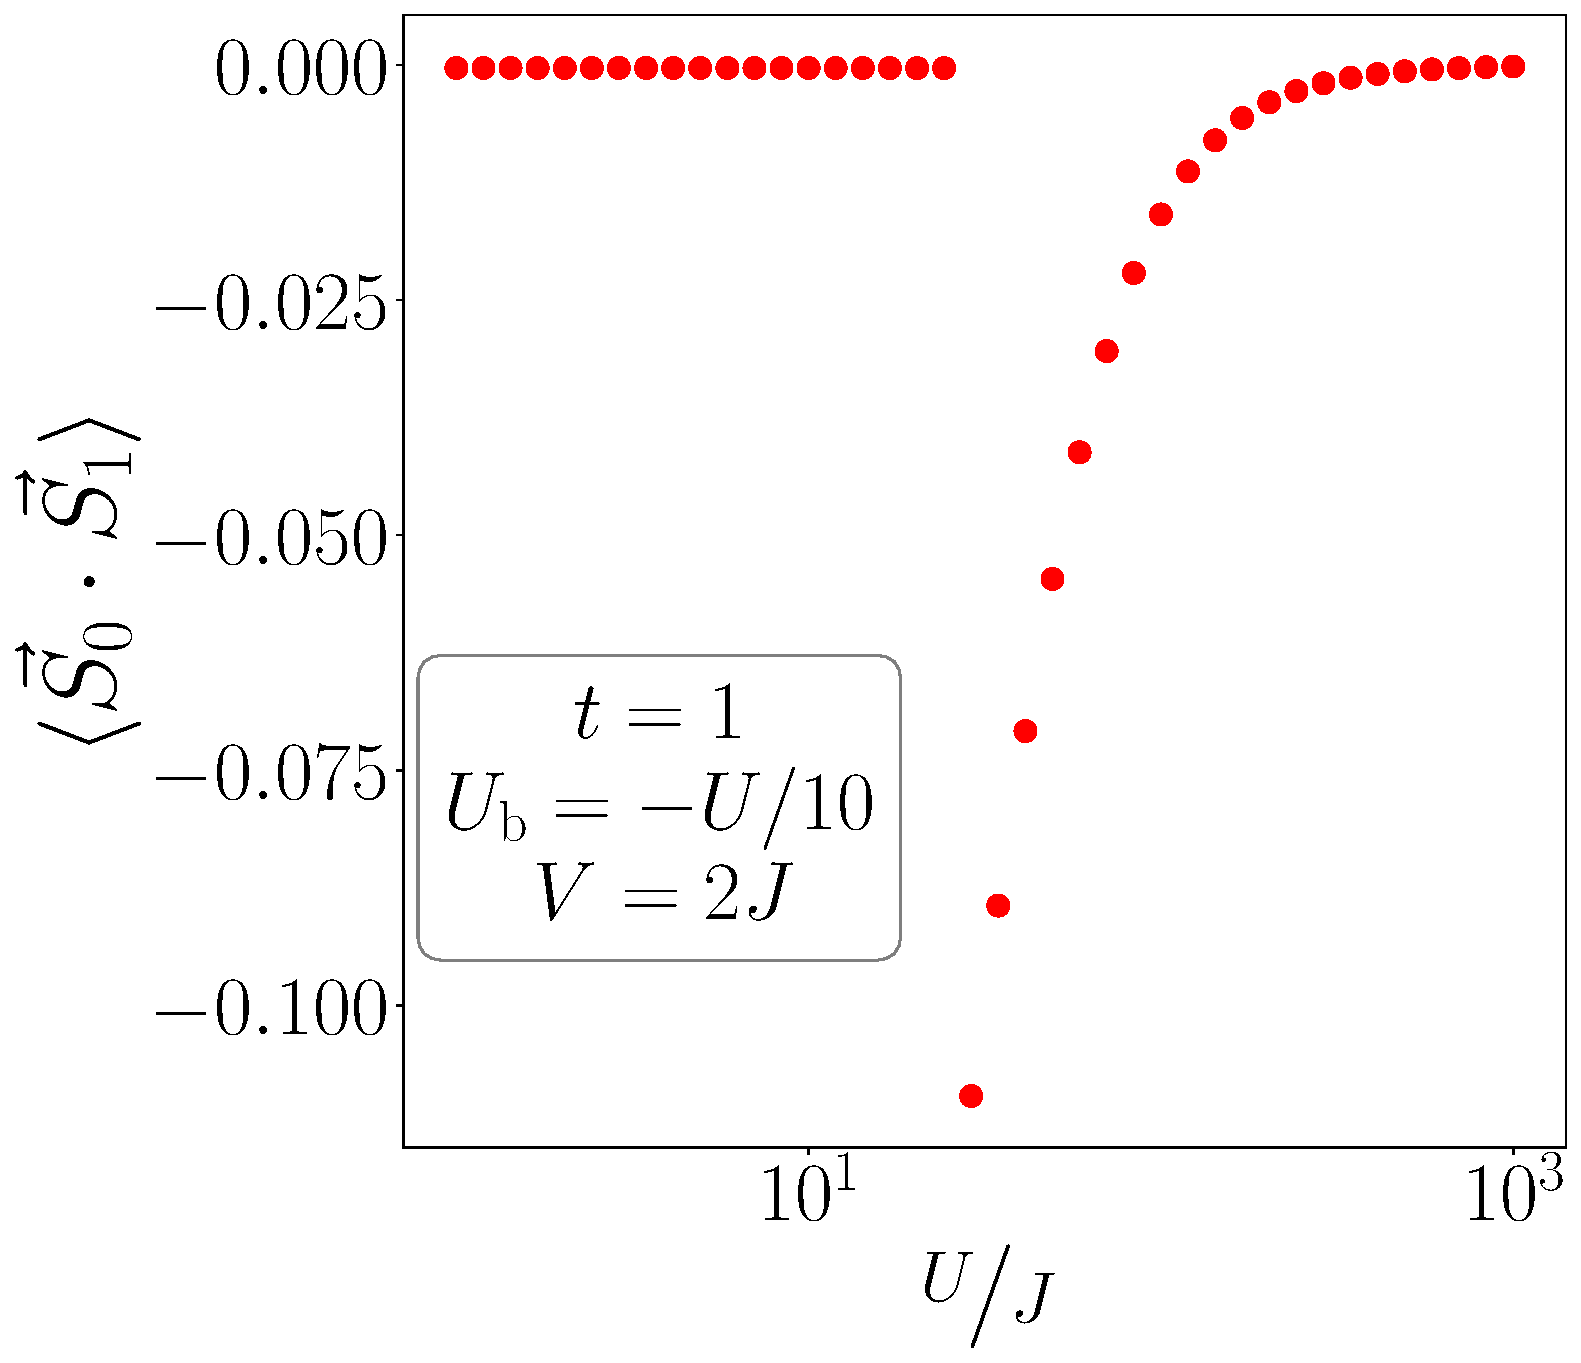
\includegraphics[width=0.32\textwidth]{./figures/r-vec-corr-01-t=1.000,J=10.000,0.000,40,V=3J,Ubath=-U_by_10,N=4,U=1.000,1000.000,40.pdf}
\end{frame}


\begin{frame}[noframenumbering]{Correlation measures: Real-space correlations}
\vspace*{20pt}
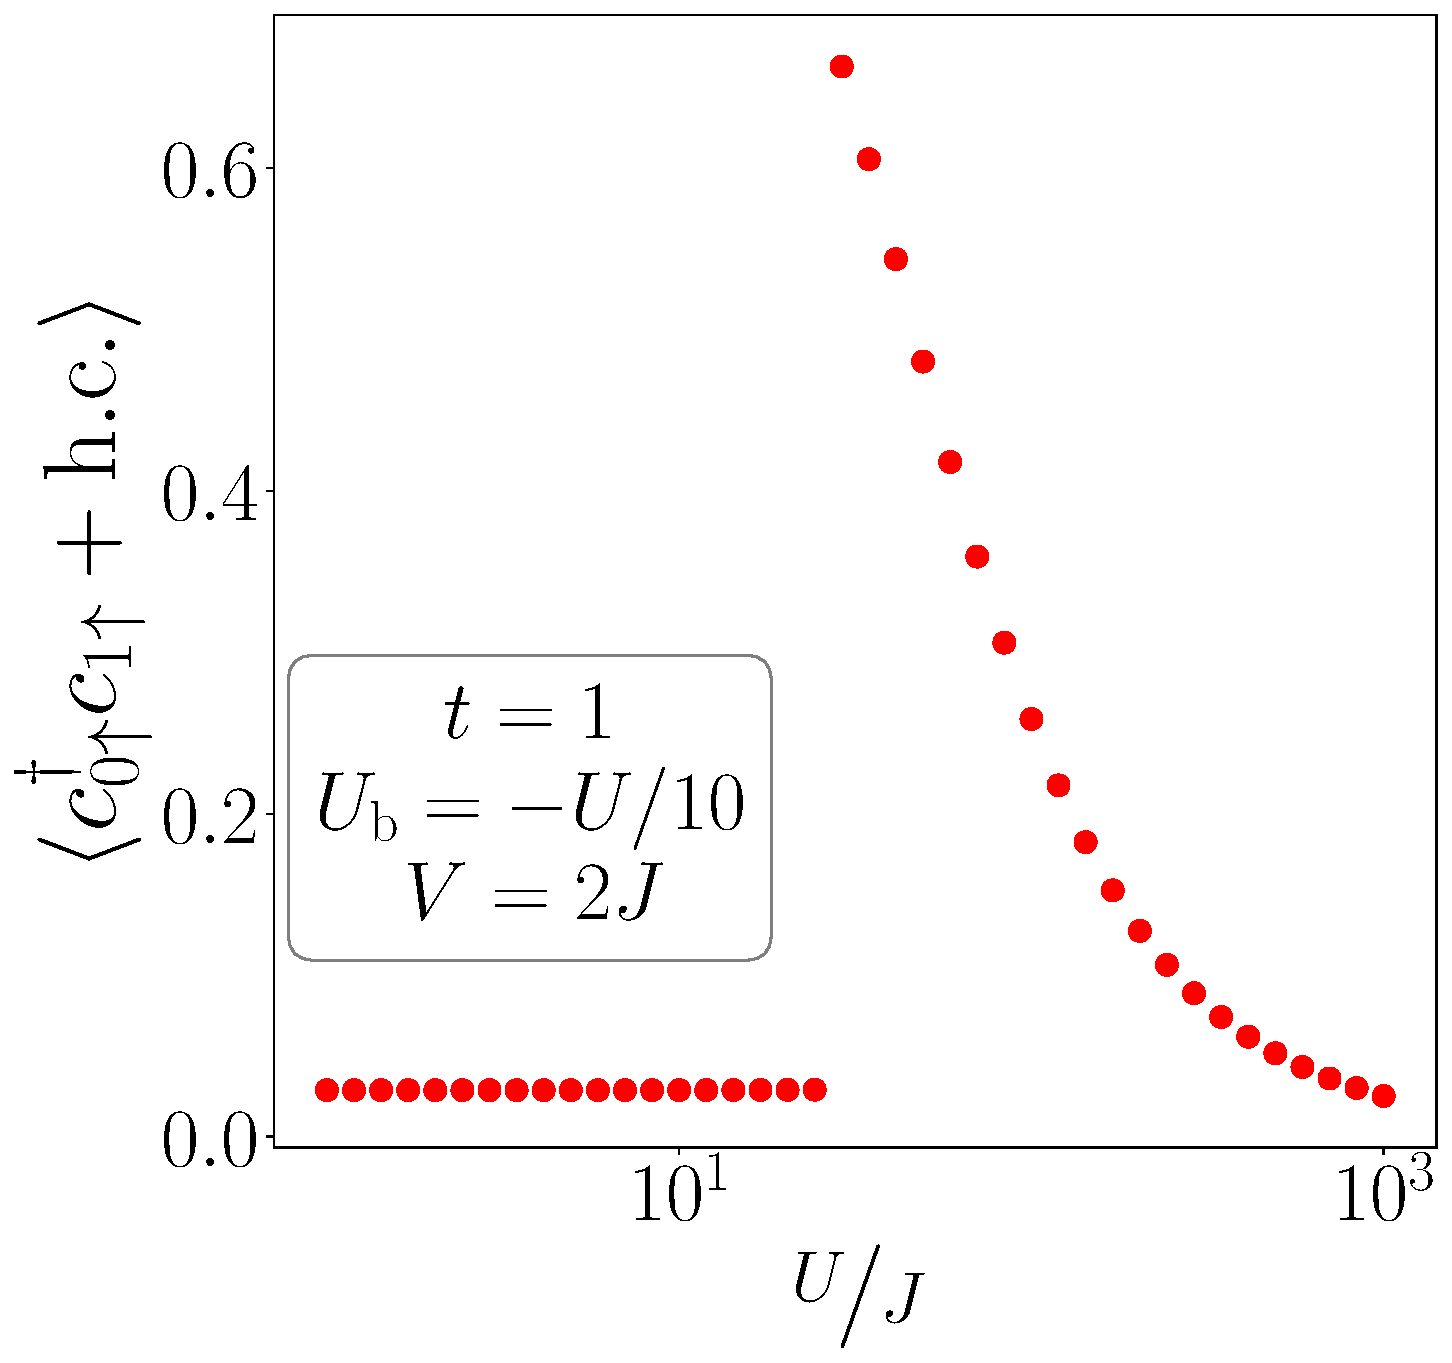
\includegraphics[width=0.49\textwidth]{./figures/r1p-t=1.000,J=10.000,0.000,40,V=3J,Ubath=-U_by_10,N=4,U=1.000,1000.000,40.pdf}
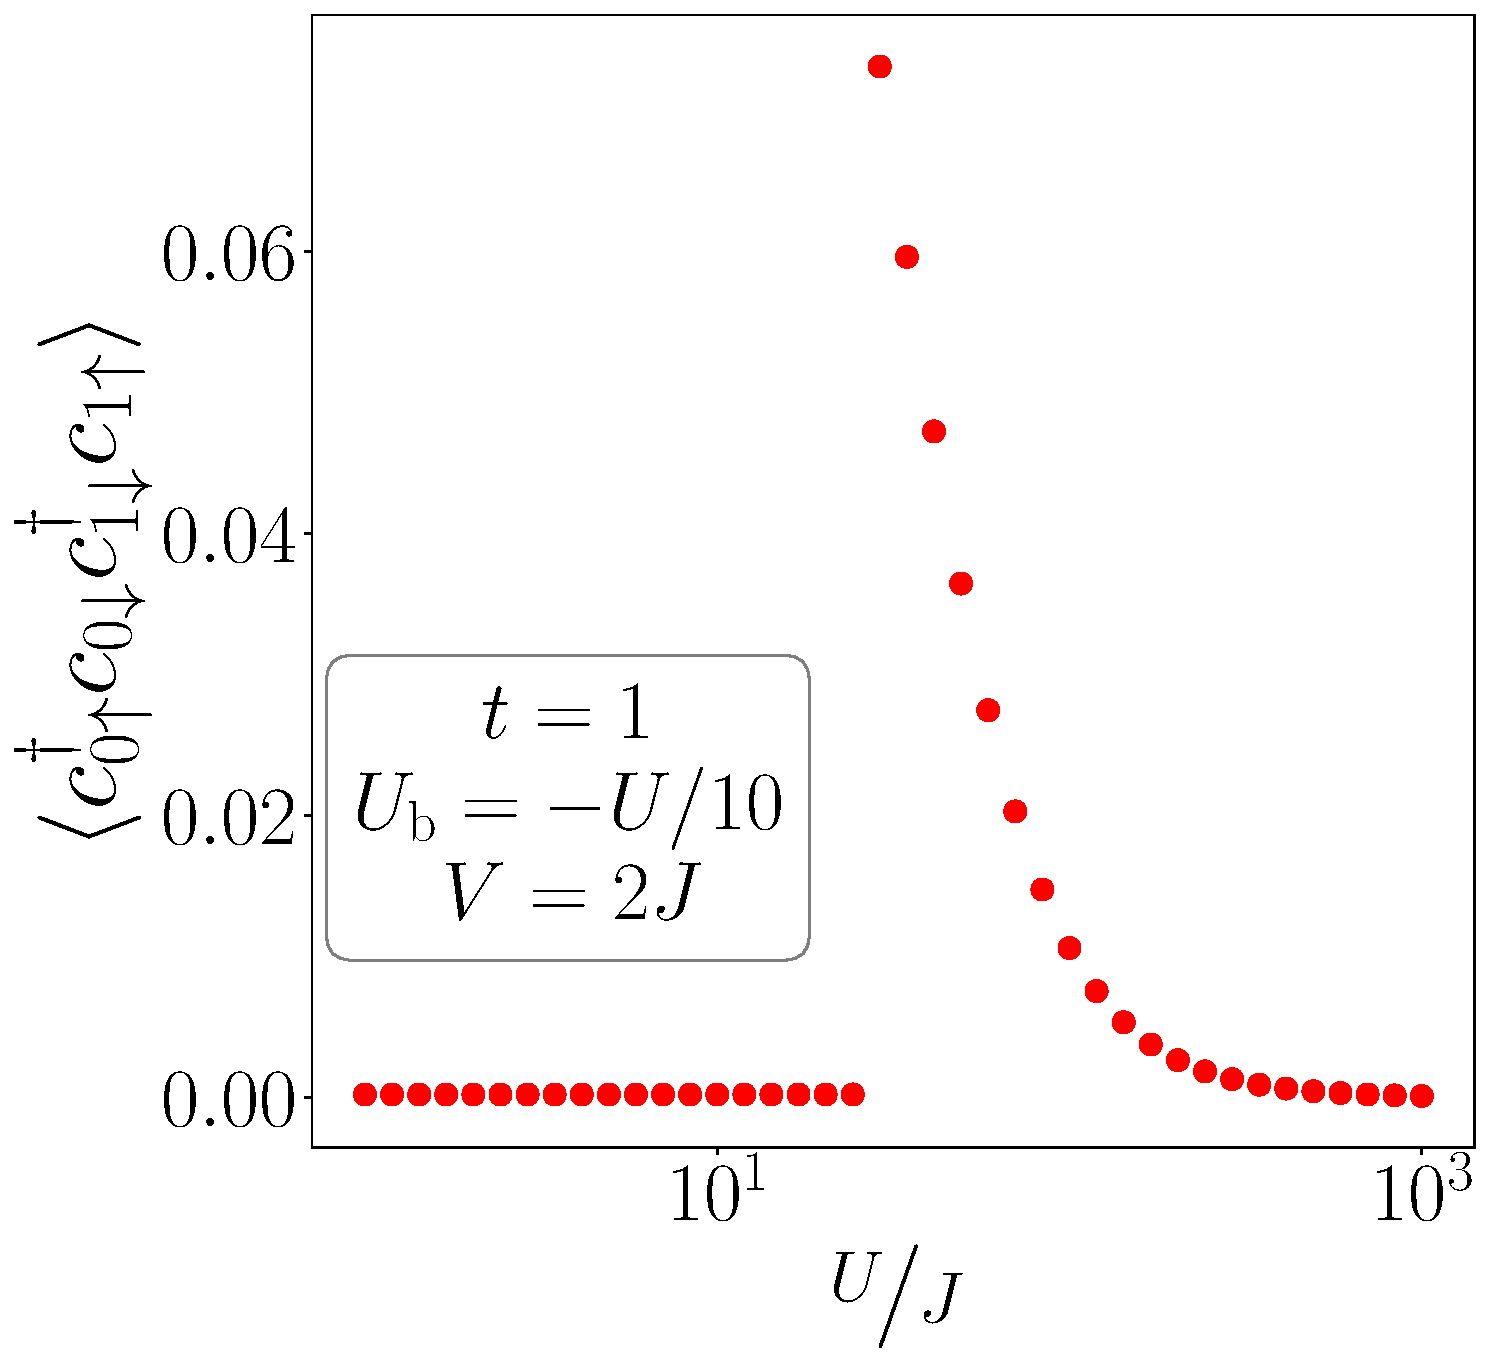
\includegraphics[width=0.49\textwidth]{./figures/r-od-t=1.000,J=10.000,0.000,40,V=3J,Ubath=-U_by_10,N=4,U=1.000,1000.000,40.pdf}
\end{frame}


\begin{frame}[noframenumbering]{Correlation measures: Impurity spectral function}
\centering
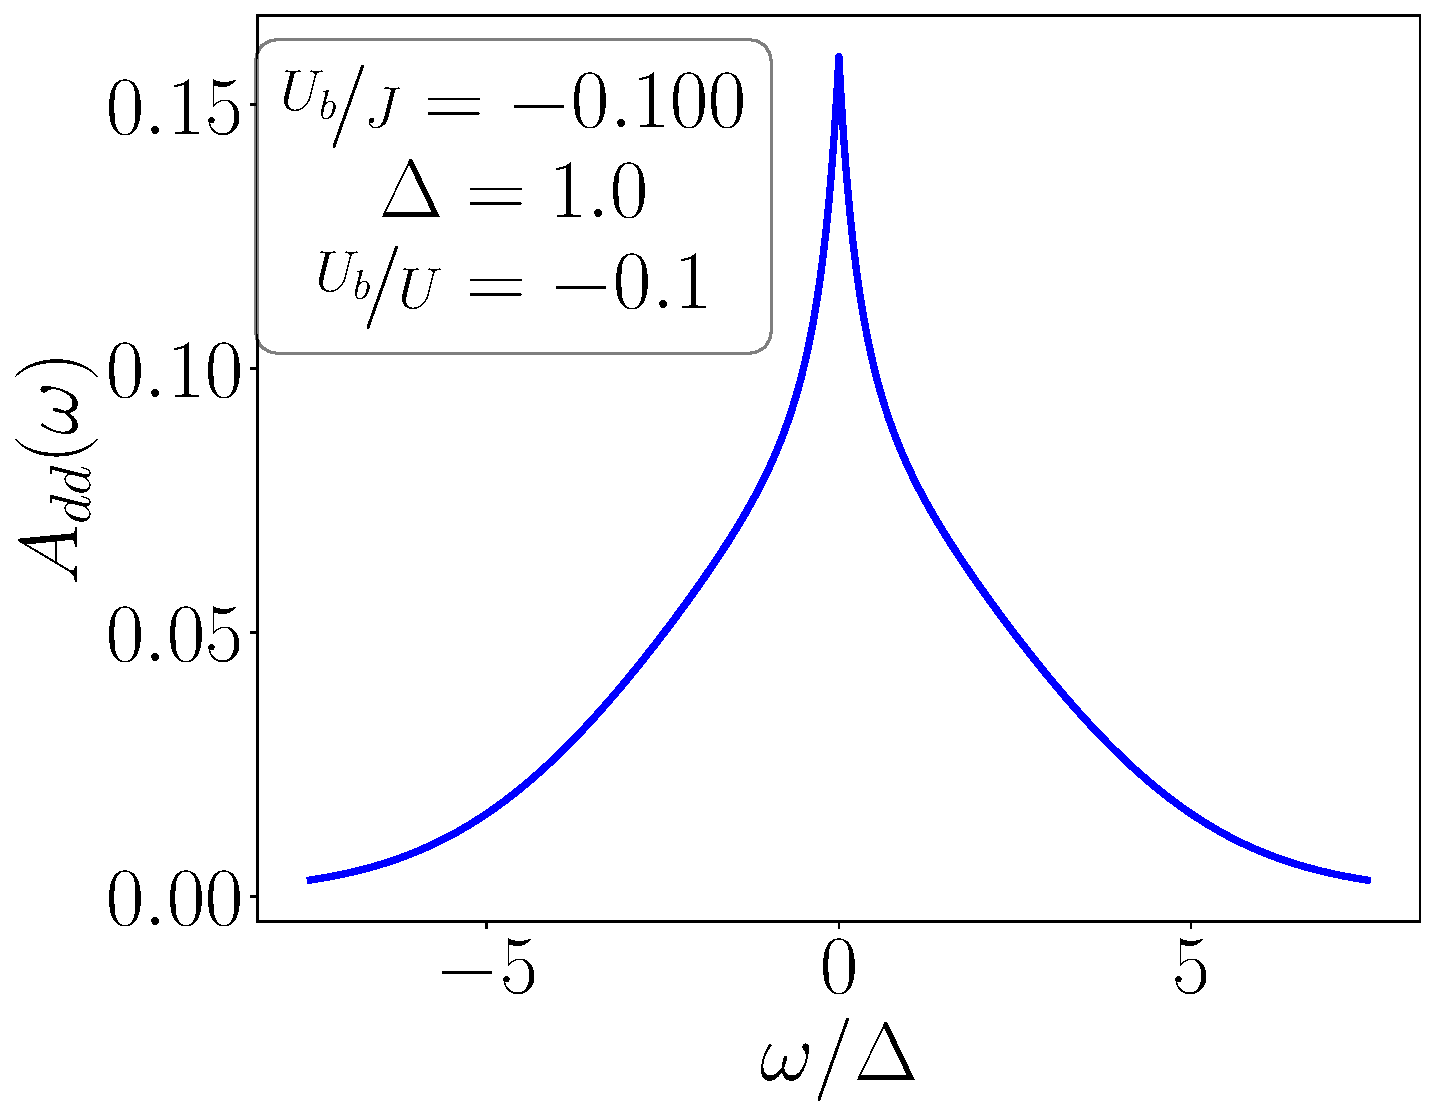
\includegraphics[width=0.32\textwidth]{./figures/spec_func_Ub_by_J=-0.100.pdf}
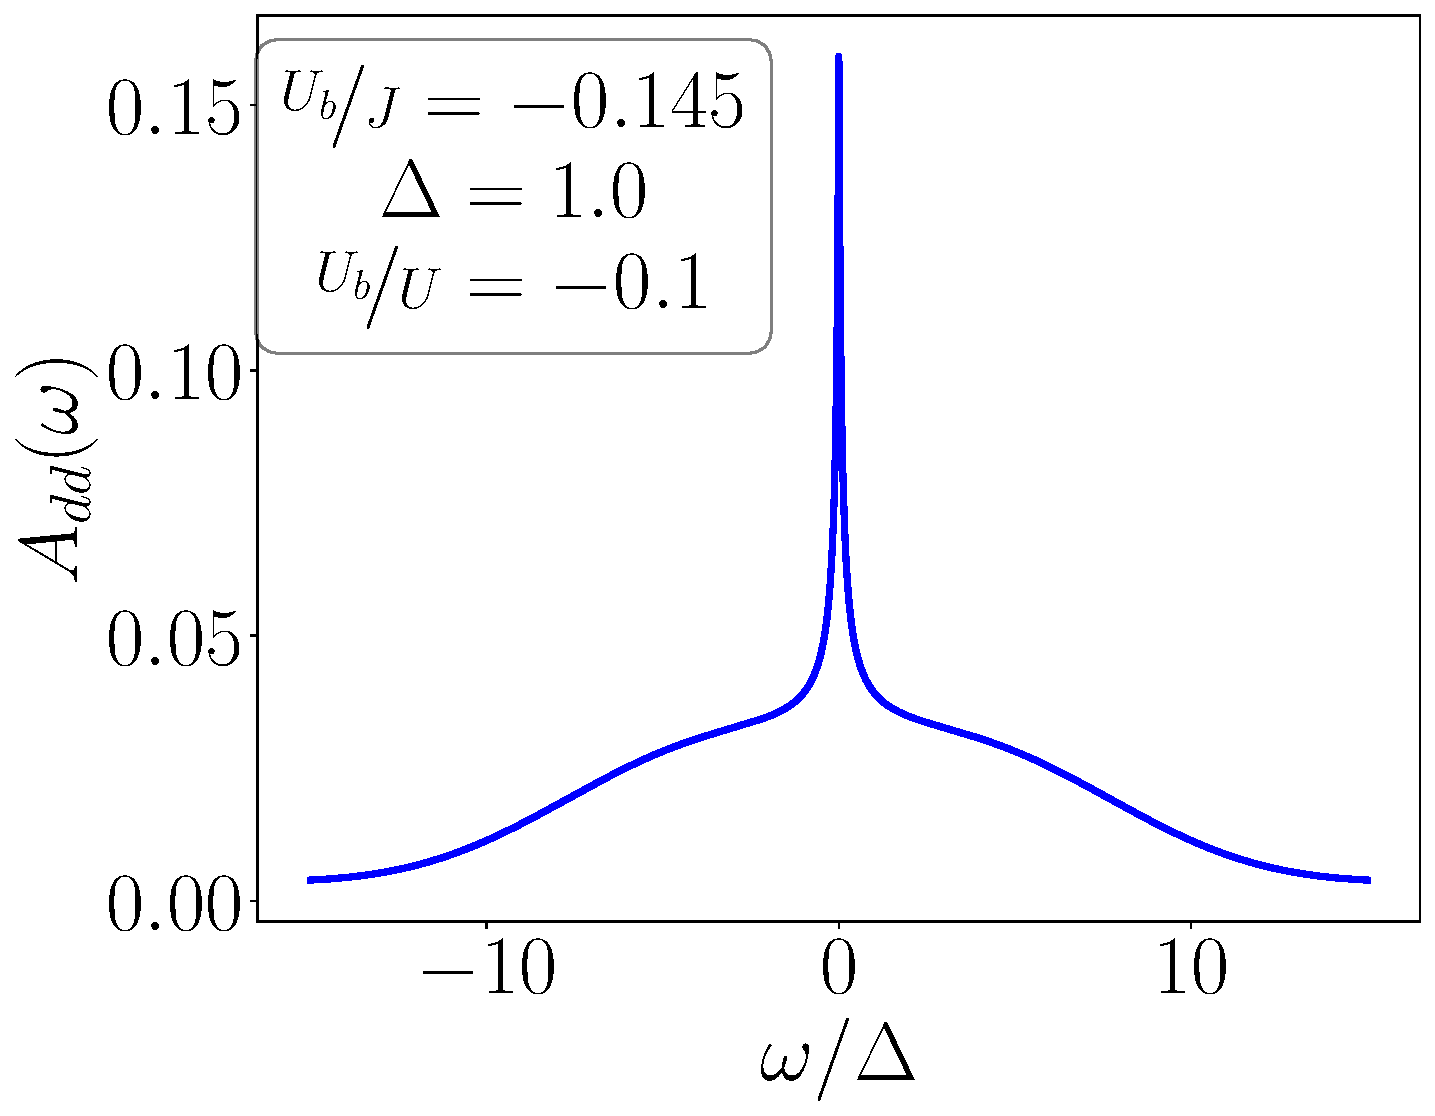
\includegraphics[width=0.32\textwidth]{./figures/spec_func_Ub_by_J=-0.145.pdf}
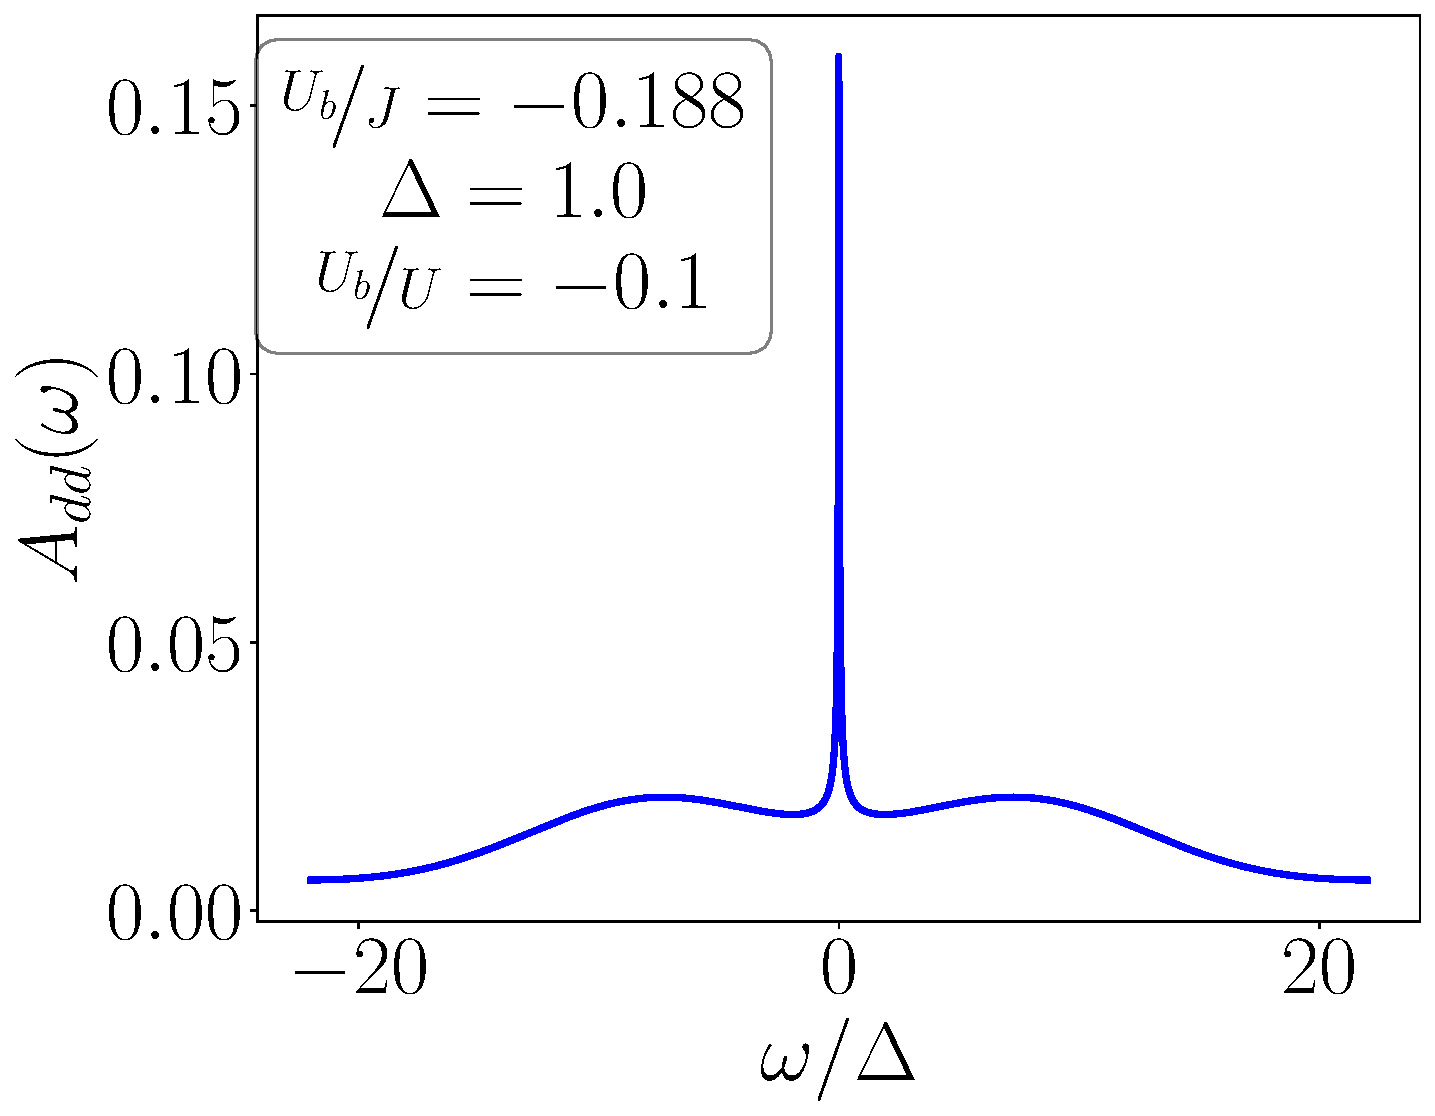
\includegraphics[width=0.32\textwidth]{./figures/spec_func_Ub_by_J=-0.188.pdf}
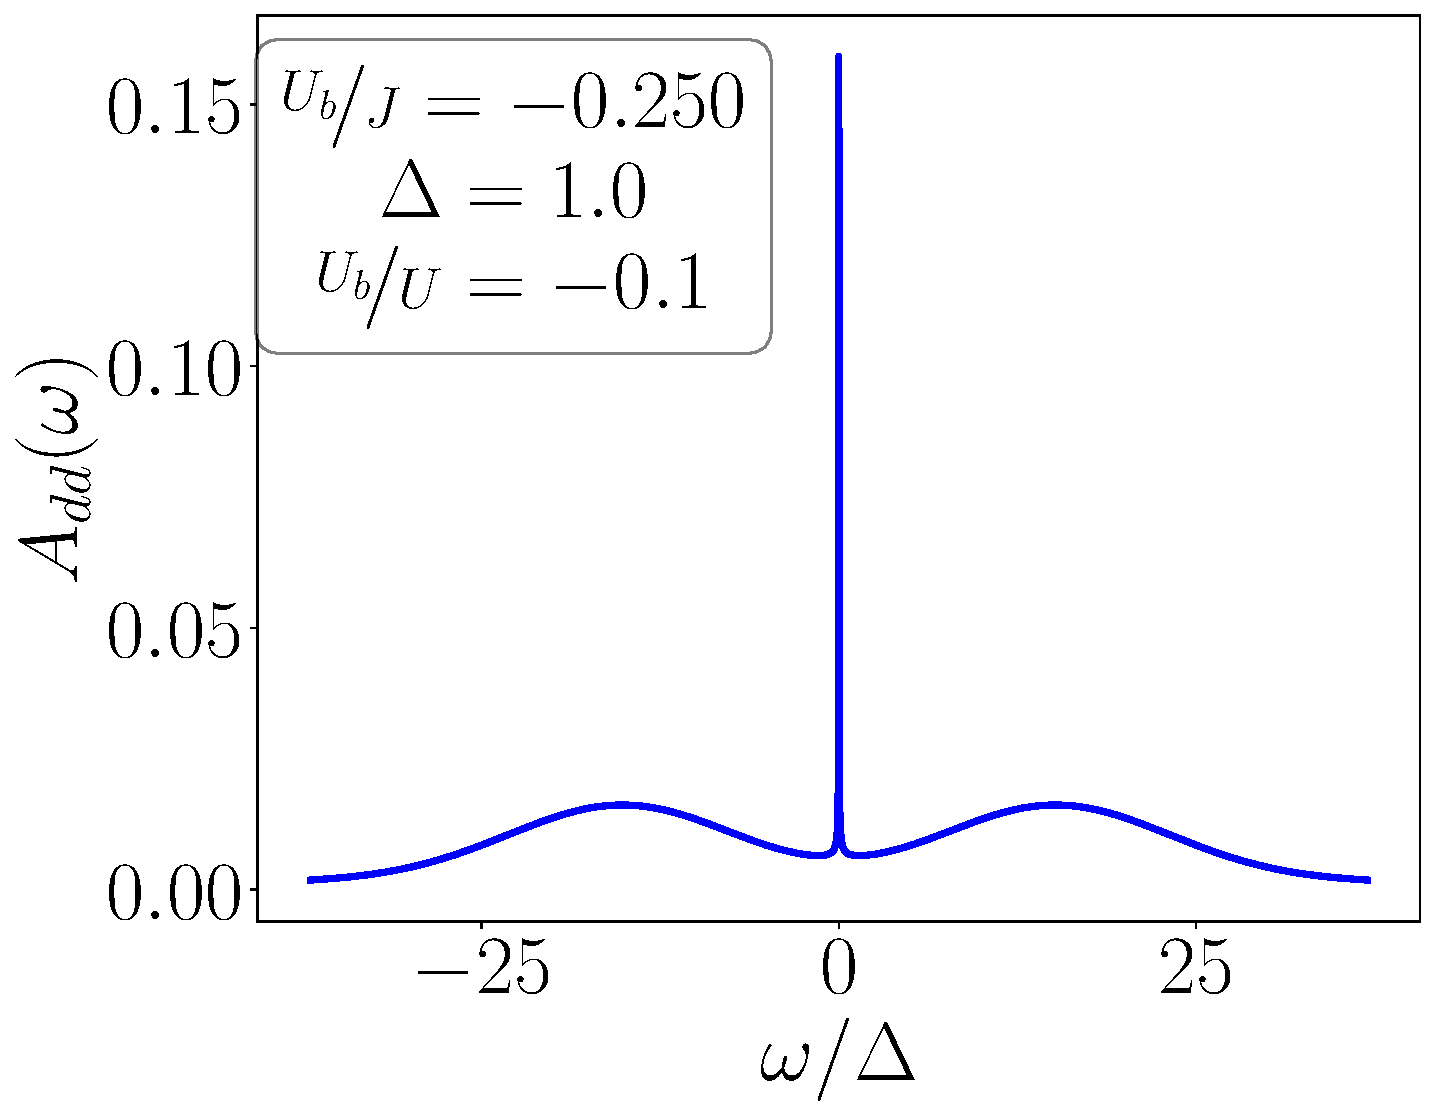
\includegraphics[width=0.32\textwidth]{./figures/spec_func_Ub_by_J=-0.250.pdf}
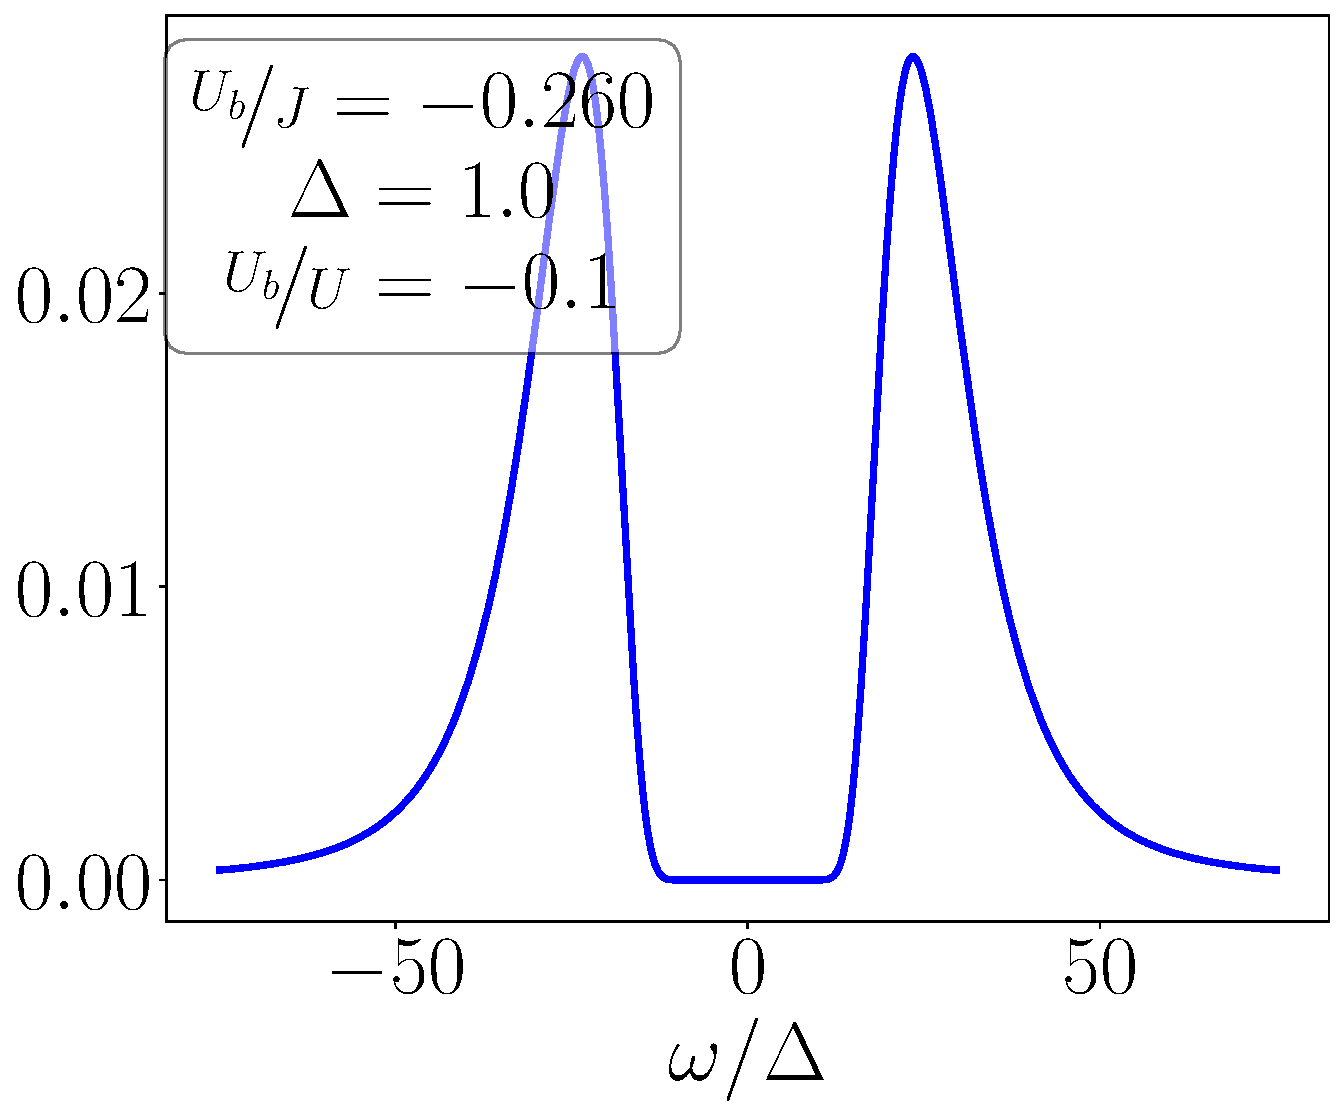
\includegraphics[width=0.32\textwidth]{./figures/spec_func_Ub_by_J=-0.26.pdf}
\end{frame}


\begin{frame}[noframenumbering]{Correlation measures: Impurity-bath spectral function \(A_{d0}\)}
\centering
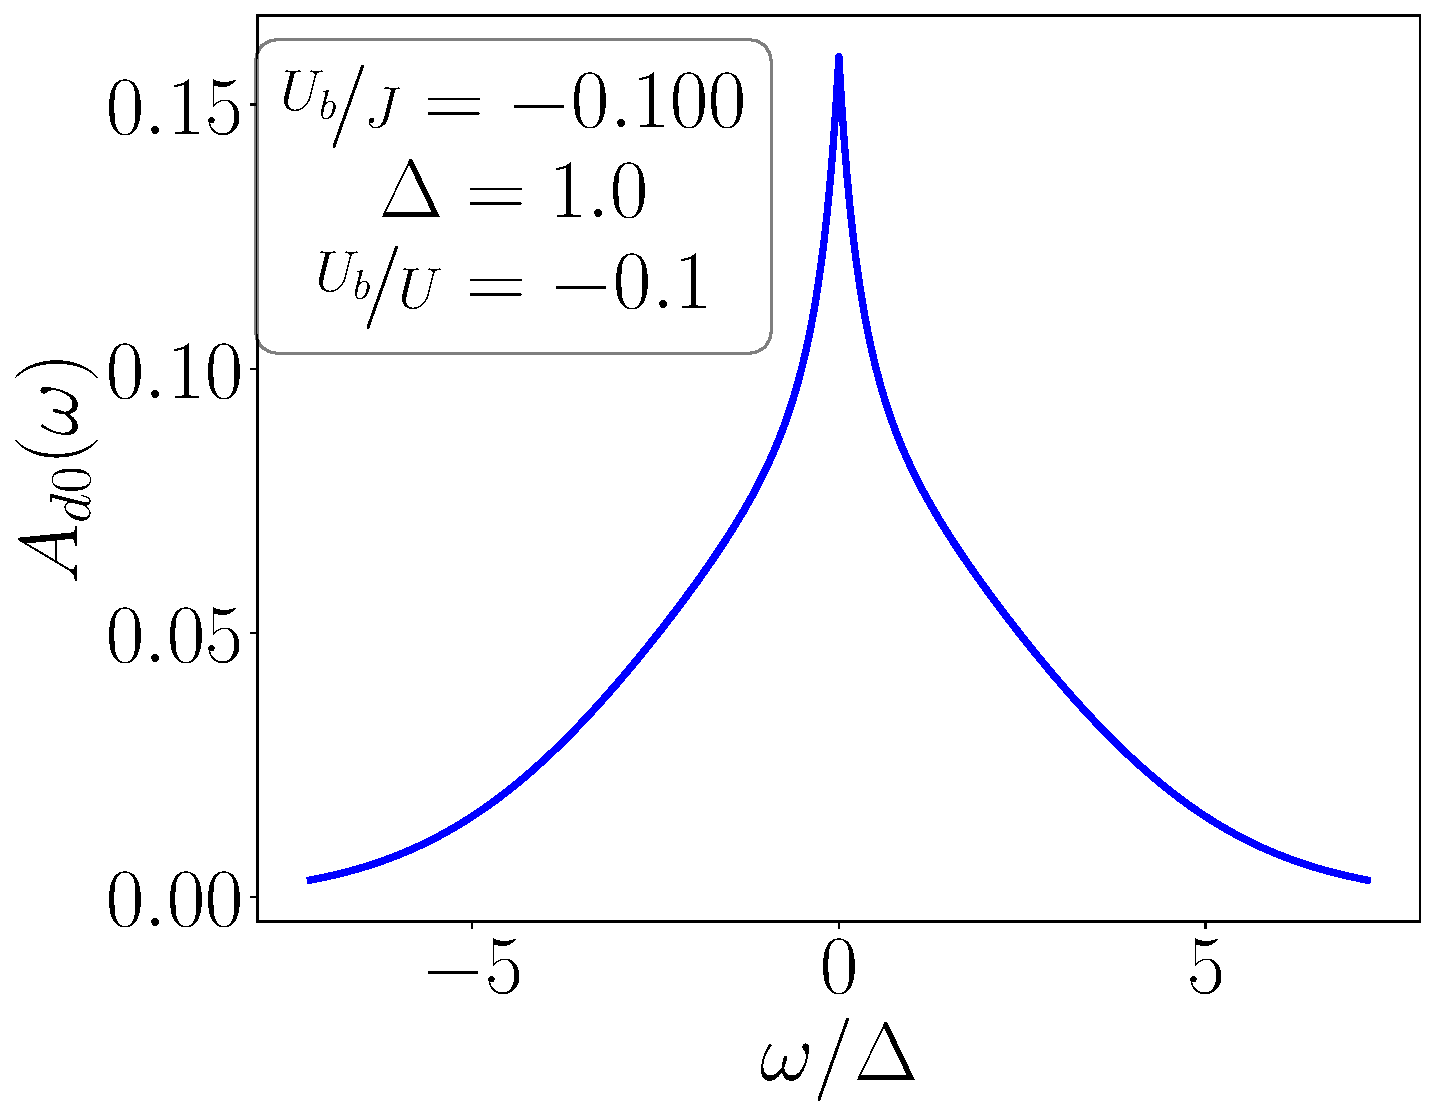
\includegraphics[width=0.32\textwidth]{./figures/spec_func_d0_Ub_by_J=-0.100.pdf}
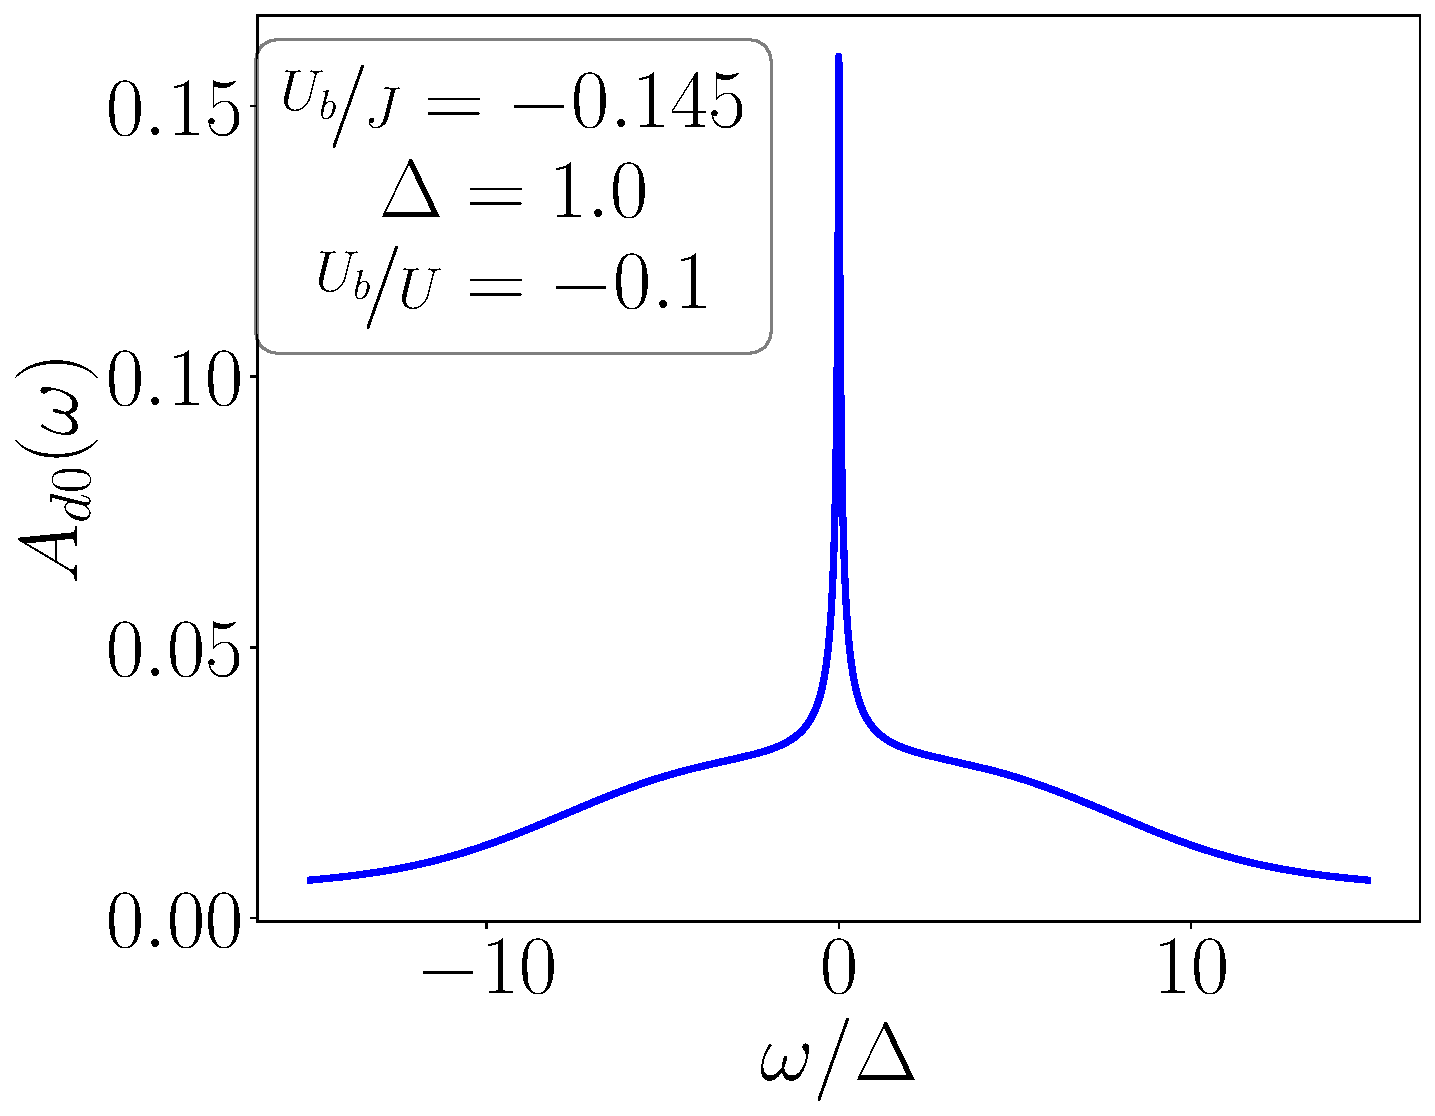
\includegraphics[width=0.32\textwidth]{./figures/spec_func_d0_Ub_by_J=-0.145.pdf}
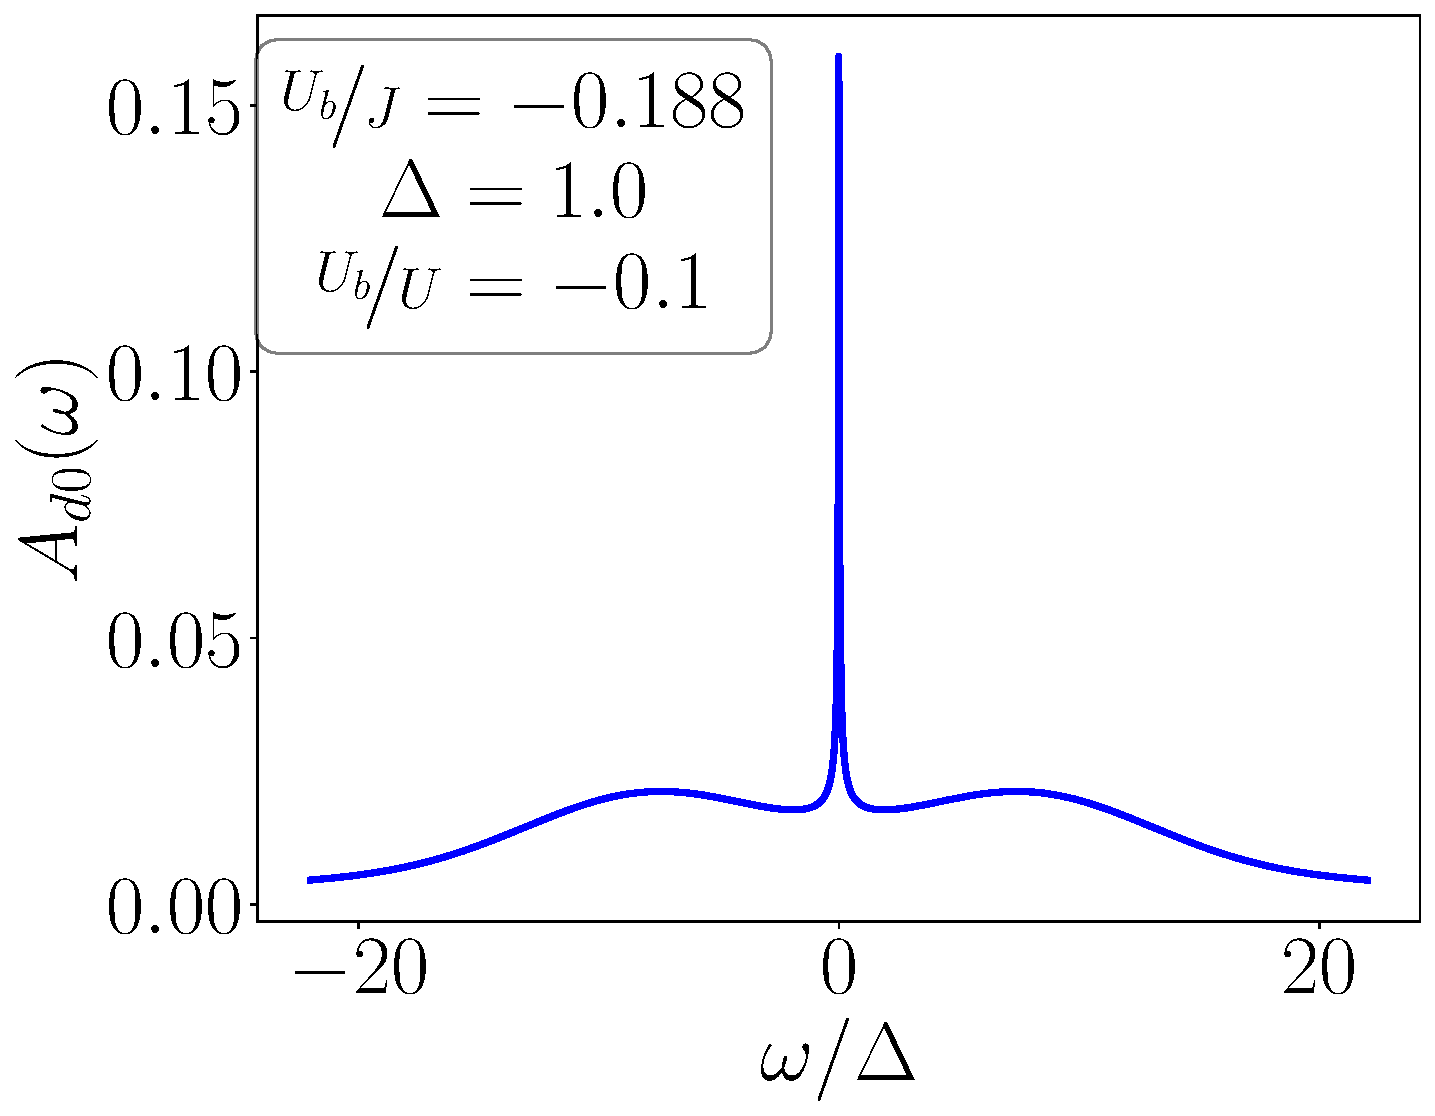
\includegraphics[width=0.32\textwidth]{./figures/spec_func_d0_Ub_by_J=-0.188.pdf}
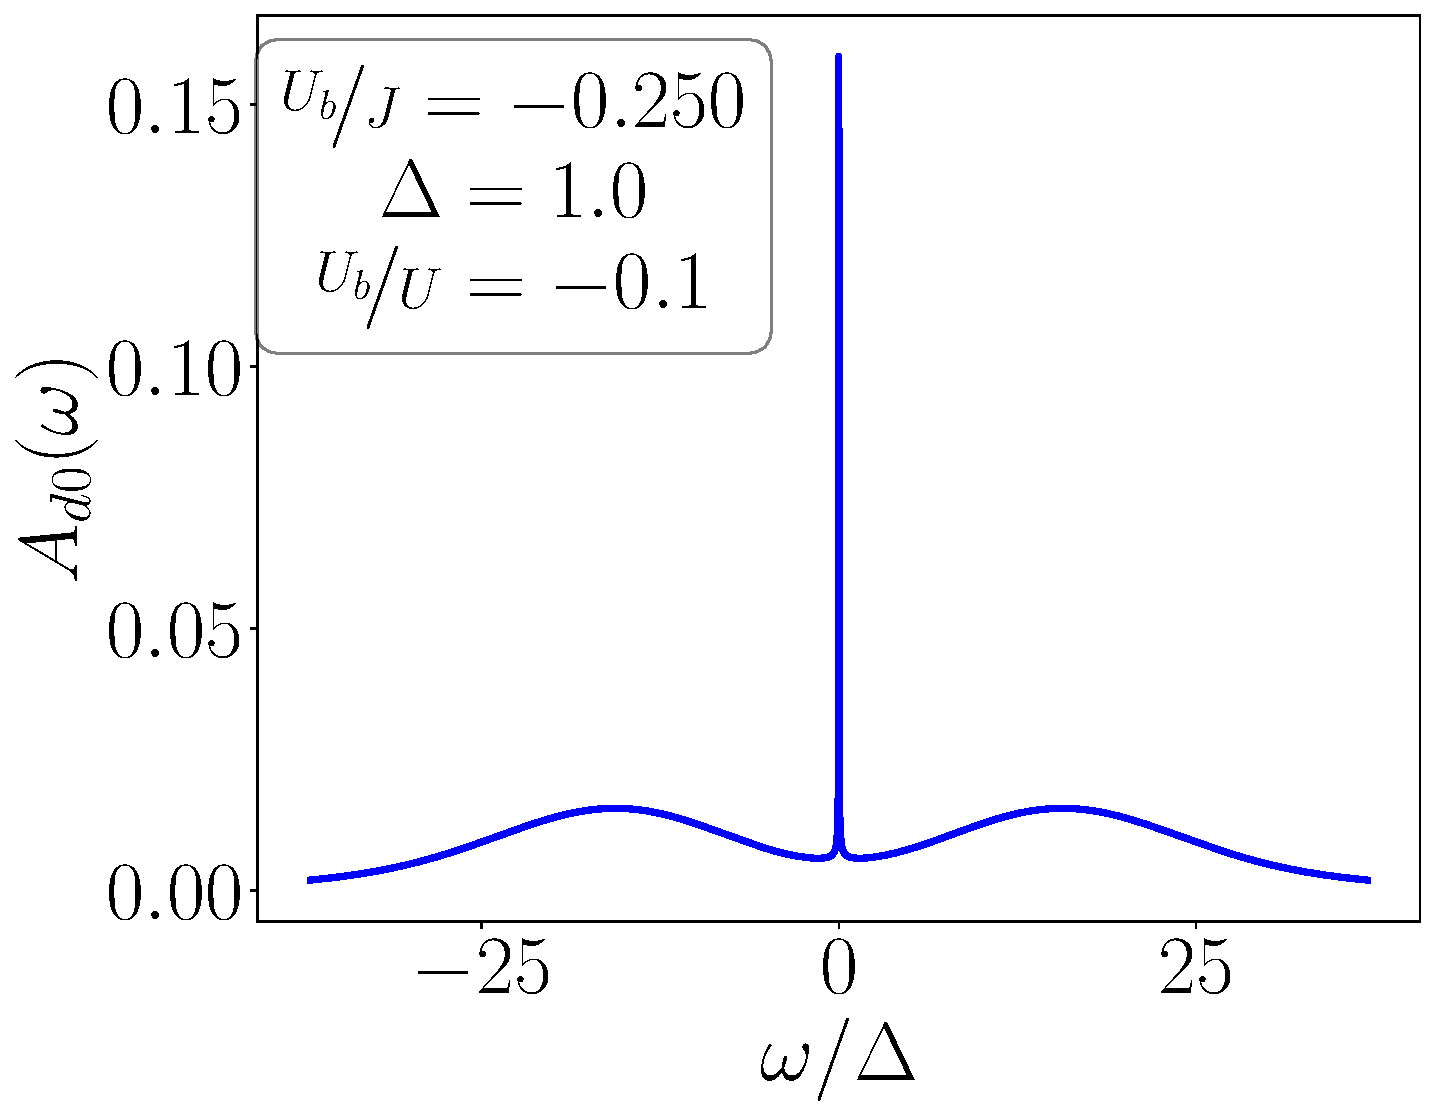
\includegraphics[width=0.32\textwidth]{./figures/spec_func_d0_Ub_by_J=-0.250.pdf}
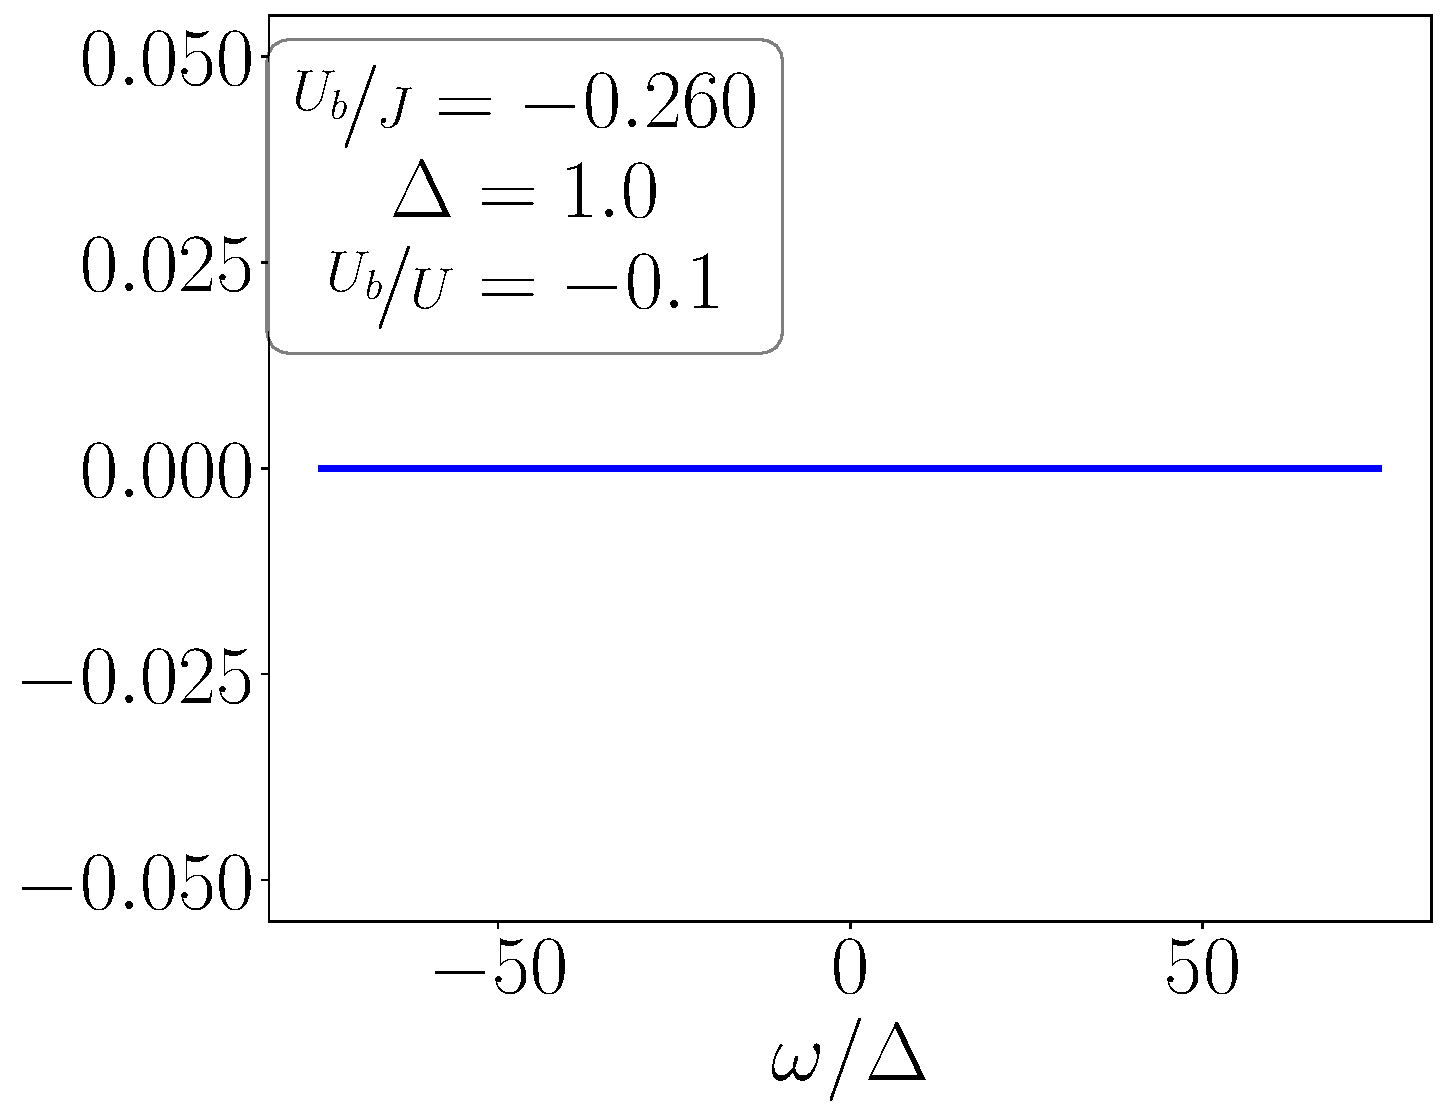
\includegraphics[width=0.32\textwidth]{./figures/spec_func_d0_Ub_by_J=-0.26.pdf}
\end{frame}


\begin{frame}[noframenumbering]{Correlation measures: Bath spectral function \(A_{00}\)}
\centering
\hspace*{\fill}
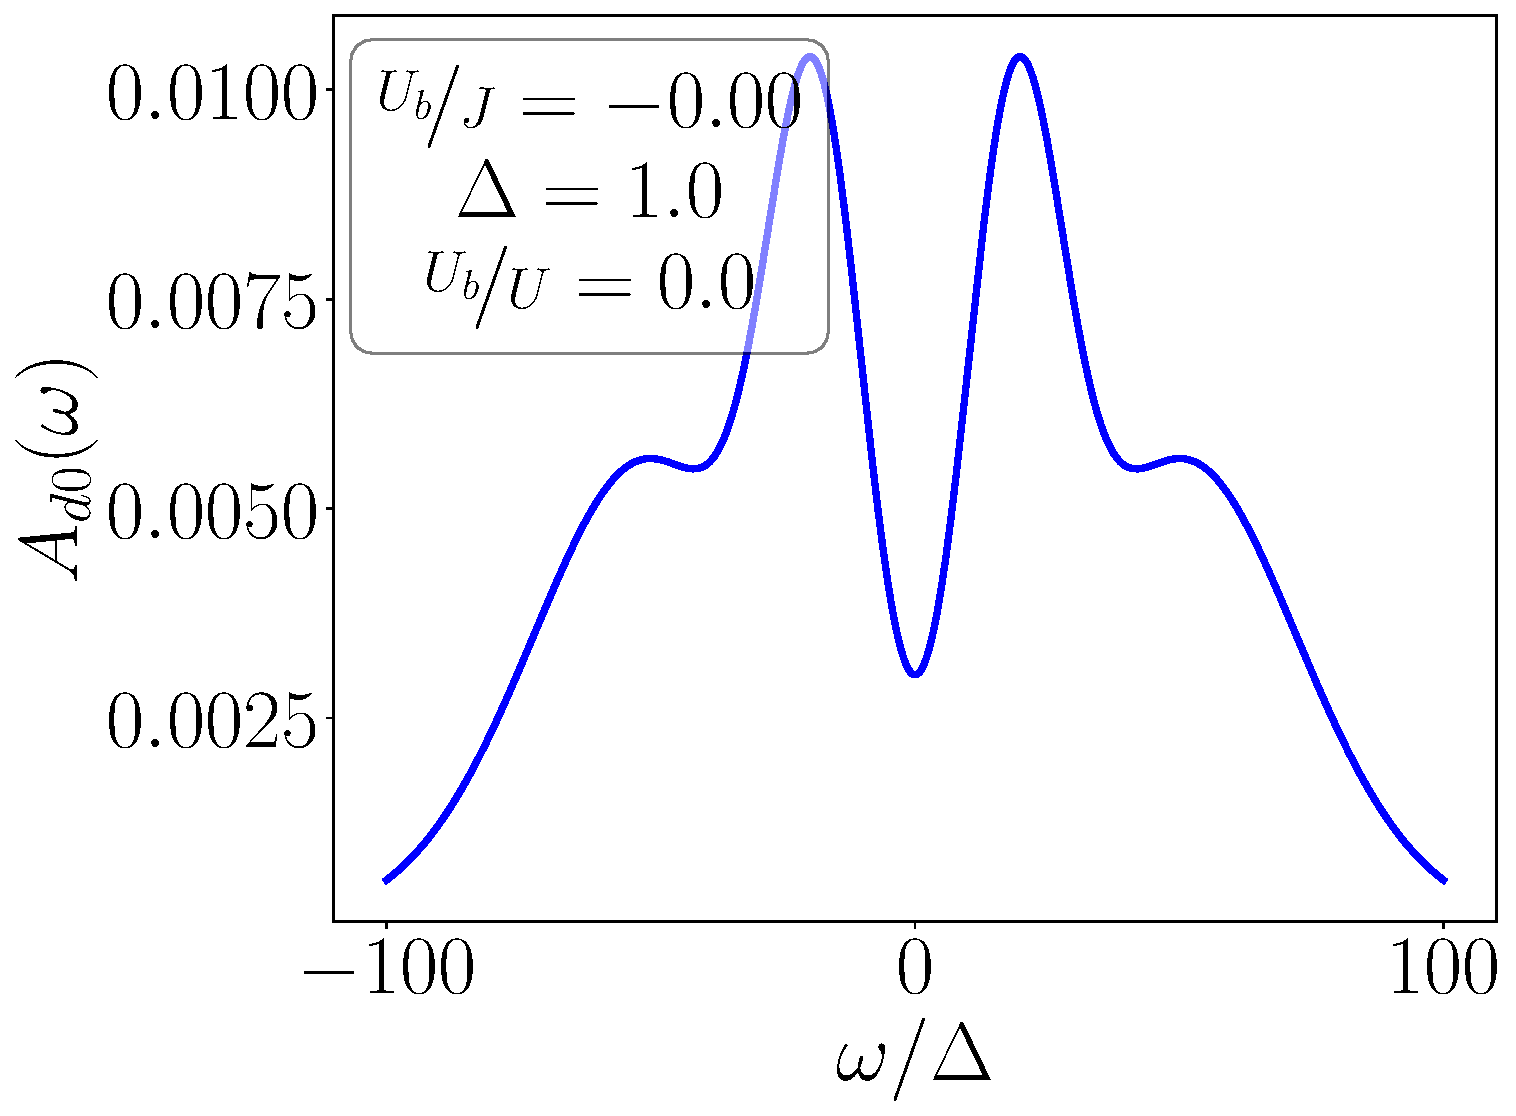
\includegraphics[width=0.33\textwidth]{./figures/spec_func_00_Ub_by_J=-0.000.pdf}
\hspace*{\fill}
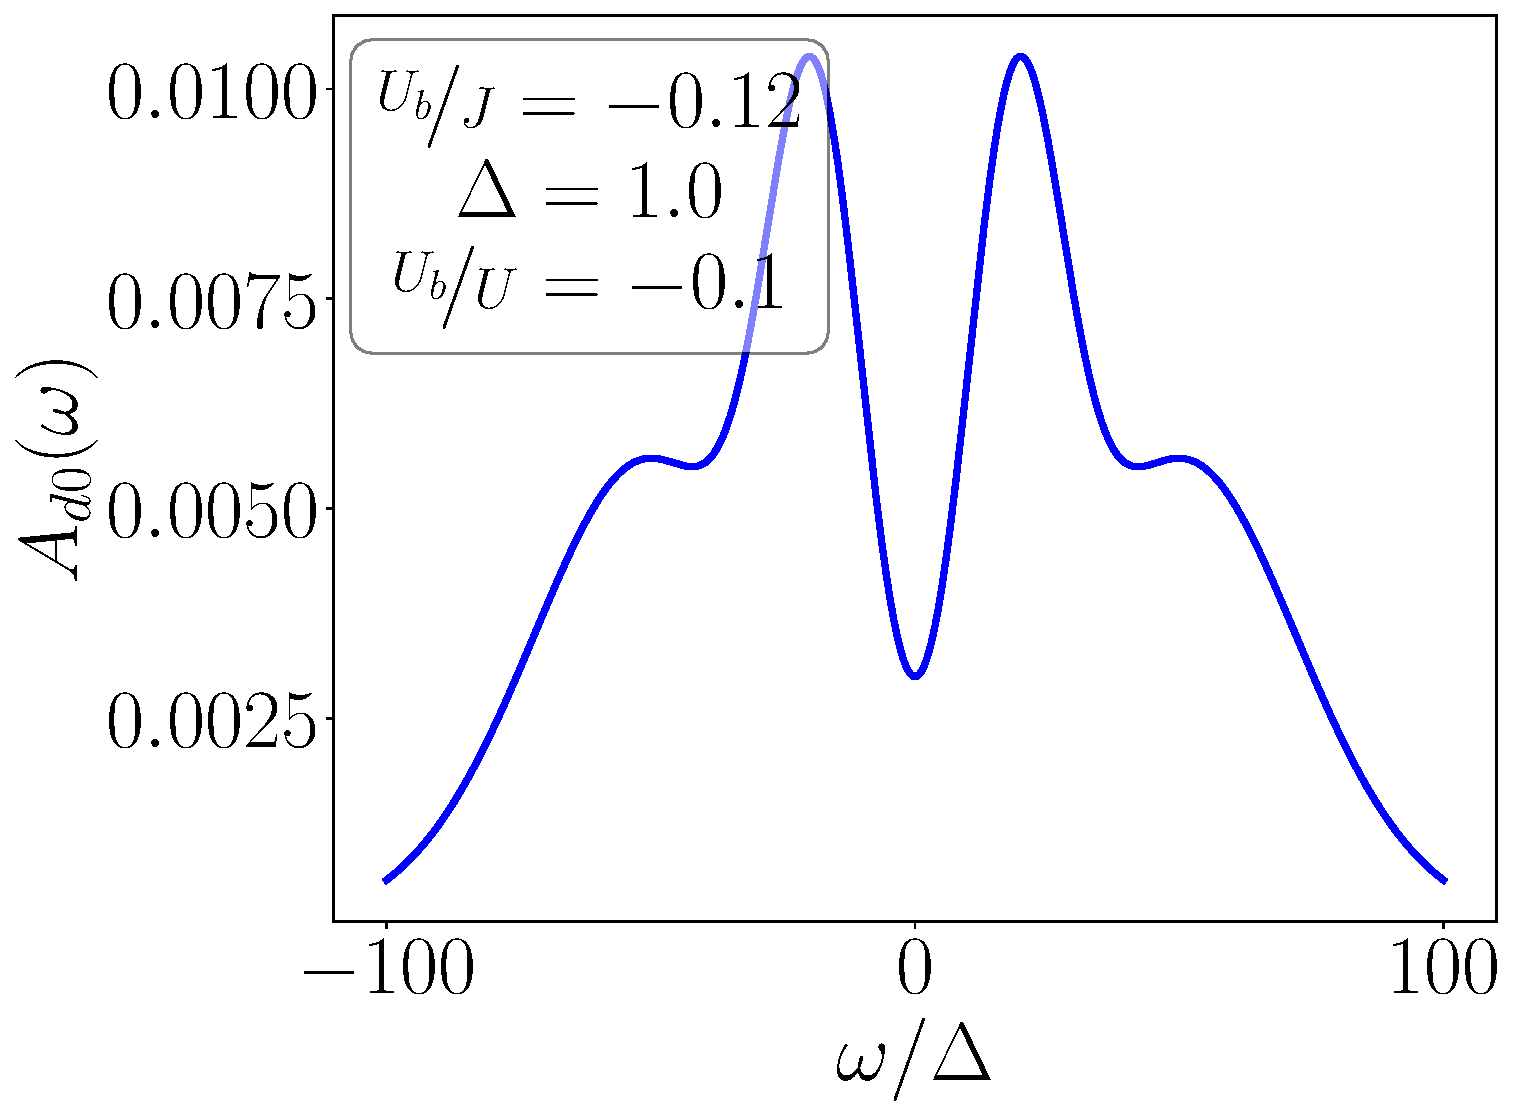
\includegraphics[width=0.33\textwidth]{./figures/spec_func_00_Ub_by_J=-0.125.pdf}
\hspace*{\fill}

\hspace*{\fill}
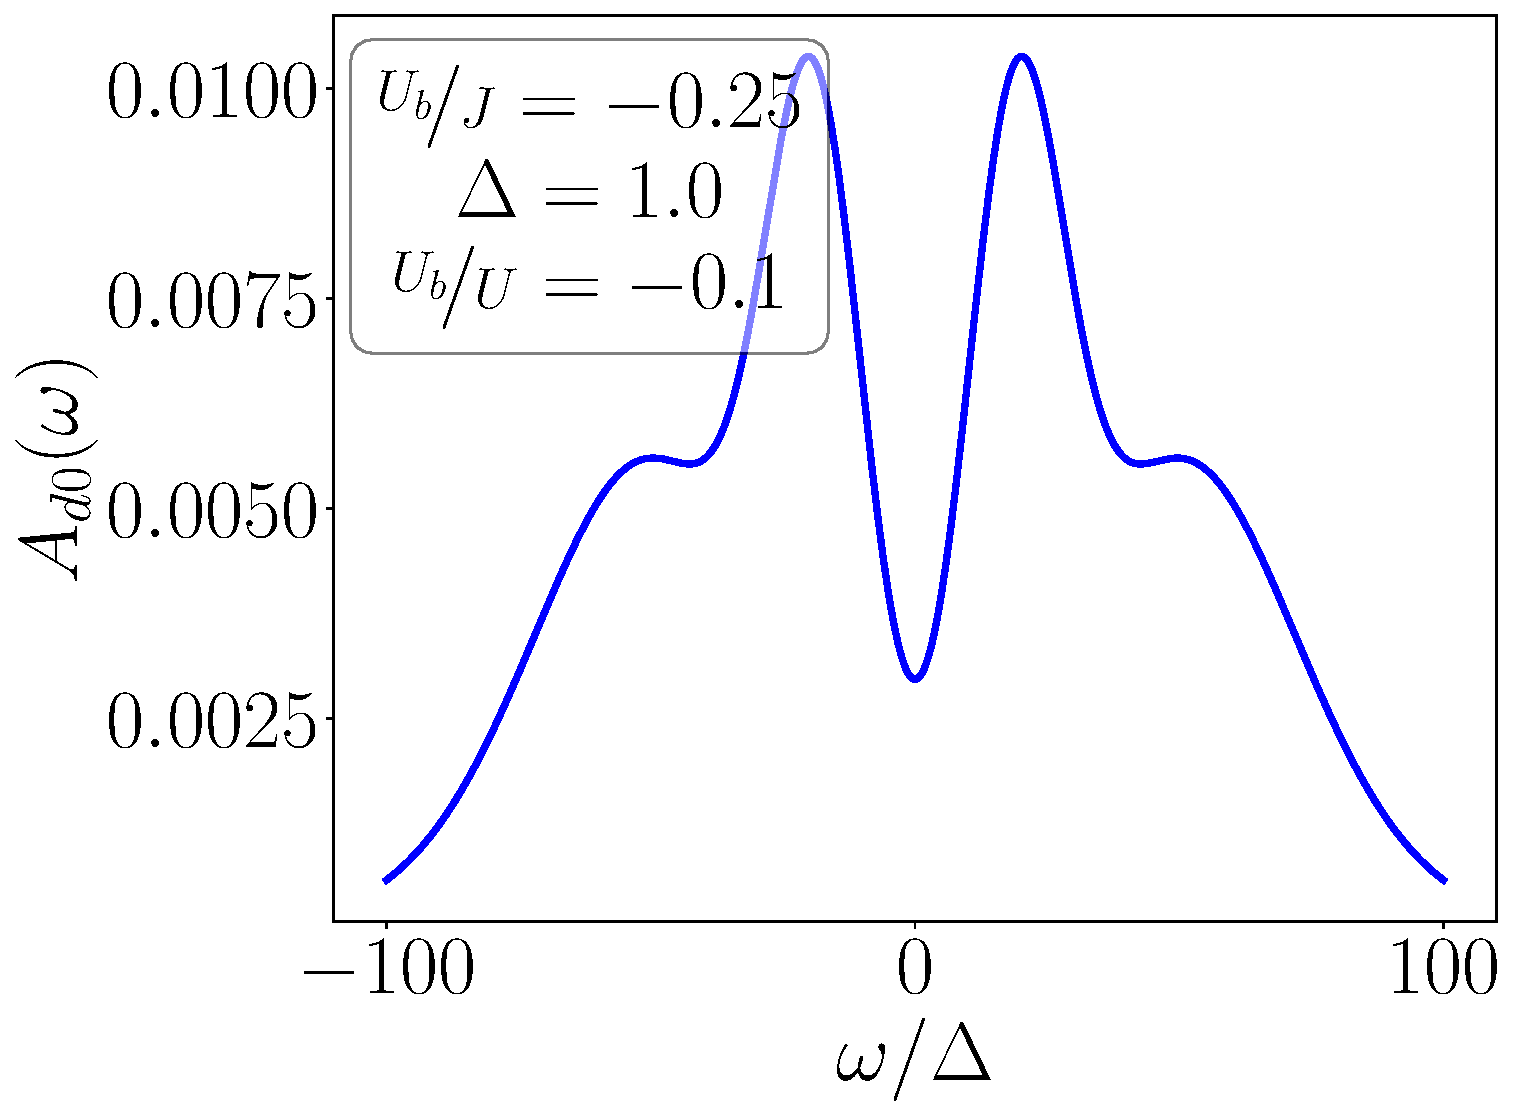
\includegraphics[width=0.33\textwidth]{./figures/spec_func_00_Ub_by_J=-0.250.pdf}
\hspace*{\fill}
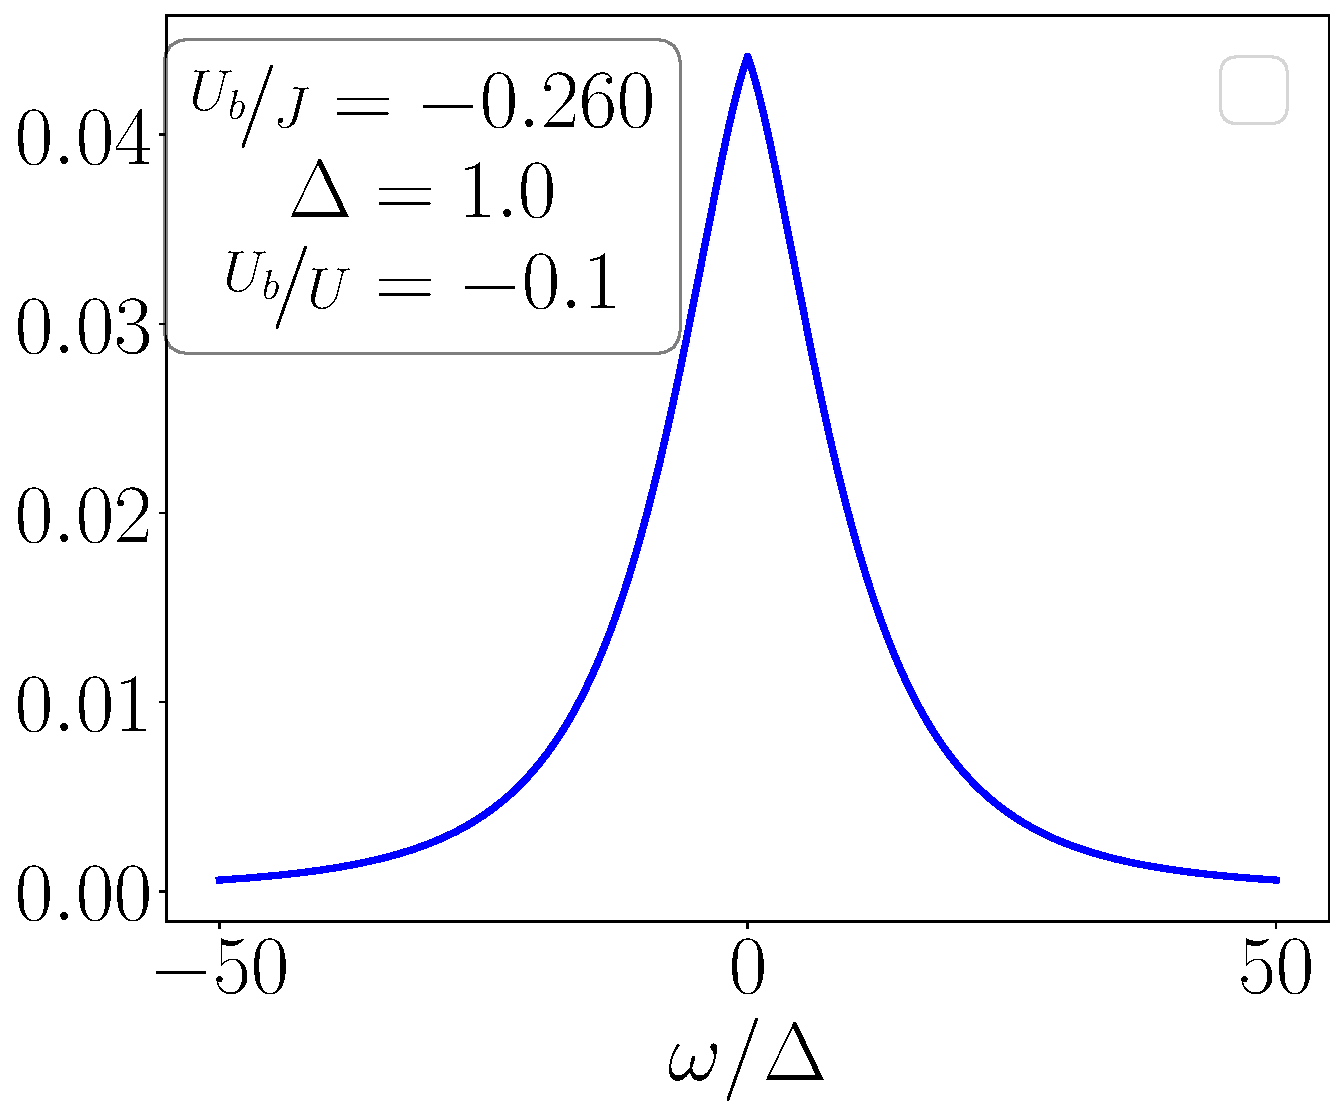
\includegraphics[width=0.29\textwidth]{./figures/spec_func_00_Ub_by_J=-0.26.pdf}
\hspace*{\fill}
\end{frame}

\section{Final Remarks}
\label{concl}

\begin{frame}[noframenumbering]{Conclusions}
	\begin{itemize}[<+->]
		\item The auxiliary model method described here provides a \focus{constructionist} approach to studying systems of strong correlations
		\item \focus{Minimal attractive interaction} on bath leads to a metal-insulator transition in the Hubbard-Heisenberg model
		\item The transition derives from a competition between \focus{Kondo} spin-flip physics and the physics of \focus{pairing} instability.
\end{itemize}
\end{frame}

\begin{frame}[noframenumbering]{Moving forward}
\begin{itemize}[<+->]
	\item \(k-\)dependence of the self-energy: \focus{electronic differentiation} and effects of Van Hove singularities?
	\item Breaking particle-hole symmetry on the impurity will allow us to study bulk models \focus{away from half-filling}.
	\item For more accurate results, one can consider \focus{multiple impurities} in the cluster.
\end{itemize}
\only<3>{\centering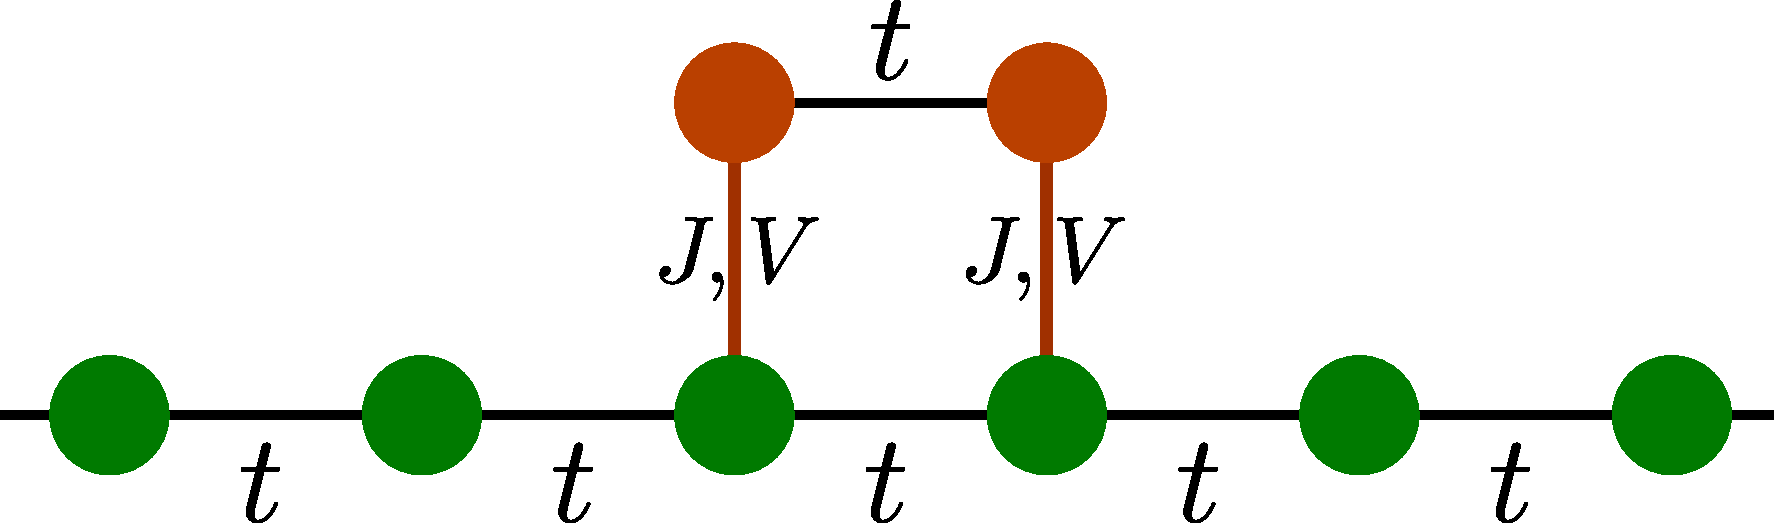
\includegraphics[height=0.3\textheight]{./figures/dimer_dispersion.pdf}}
\end{frame}

\section{Thank you.}


\end{document}
